% Options for packages loaded elsewhere
\PassOptionsToPackage{unicode}{hyperref}
\PassOptionsToPackage{hyphens}{url}
\PassOptionsToPackage{dvipsnames,svgnames,x11names}{xcolor}
%
\documentclass[
  letterpaper,
  DIV=11,
  numbers=noendperiod]{scrreprt}

\usepackage{amsmath,amssymb}
\usepackage{iftex}
\ifPDFTeX
  \usepackage[T1]{fontenc}
  \usepackage[utf8]{inputenc}
  \usepackage{textcomp} % provide euro and other symbols
\else % if luatex or xetex
  \usepackage{unicode-math}
  \defaultfontfeatures{Scale=MatchLowercase}
  \defaultfontfeatures[\rmfamily]{Ligatures=TeX,Scale=1}
\fi
\usepackage{lmodern}
\ifPDFTeX\else  
    % xetex/luatex font selection
\fi
% Use upquote if available, for straight quotes in verbatim environments
\IfFileExists{upquote.sty}{\usepackage{upquote}}{}
\IfFileExists{microtype.sty}{% use microtype if available
  \usepackage[]{microtype}
  \UseMicrotypeSet[protrusion]{basicmath} % disable protrusion for tt fonts
}{}
\makeatletter
\@ifundefined{KOMAClassName}{% if non-KOMA class
  \IfFileExists{parskip.sty}{%
    \usepackage{parskip}
  }{% else
    \setlength{\parindent}{0pt}
    \setlength{\parskip}{6pt plus 2pt minus 1pt}}
}{% if KOMA class
  \KOMAoptions{parskip=half}}
\makeatother
\usepackage{xcolor}
\setlength{\emergencystretch}{3em} % prevent overfull lines
\setcounter{secnumdepth}{5}
% Make \paragraph and \subparagraph free-standing
\makeatletter
\ifx\paragraph\undefined\else
  \let\oldparagraph\paragraph
  \renewcommand{\paragraph}{
    \@ifstar
      \xxxParagraphStar
      \xxxParagraphNoStar
  }
  \newcommand{\xxxParagraphStar}[1]{\oldparagraph*{#1}\mbox{}}
  \newcommand{\xxxParagraphNoStar}[1]{\oldparagraph{#1}\mbox{}}
\fi
\ifx\subparagraph\undefined\else
  \let\oldsubparagraph\subparagraph
  \renewcommand{\subparagraph}{
    \@ifstar
      \xxxSubParagraphStar
      \xxxSubParagraphNoStar
  }
  \newcommand{\xxxSubParagraphStar}[1]{\oldsubparagraph*{#1}\mbox{}}
  \newcommand{\xxxSubParagraphNoStar}[1]{\oldsubparagraph{#1}\mbox{}}
\fi
\makeatother

\usepackage{color}
\usepackage{fancyvrb}
\newcommand{\VerbBar}{|}
\newcommand{\VERB}{\Verb[commandchars=\\\{\}]}
\DefineVerbatimEnvironment{Highlighting}{Verbatim}{commandchars=\\\{\}}
% Add ',fontsize=\small' for more characters per line
\usepackage{framed}
\definecolor{shadecolor}{RGB}{241,243,245}
\newenvironment{Shaded}{\begin{snugshade}}{\end{snugshade}}
\newcommand{\AlertTok}[1]{\textcolor[rgb]{0.68,0.00,0.00}{#1}}
\newcommand{\AnnotationTok}[1]{\textcolor[rgb]{0.37,0.37,0.37}{#1}}
\newcommand{\AttributeTok}[1]{\textcolor[rgb]{0.40,0.45,0.13}{#1}}
\newcommand{\BaseNTok}[1]{\textcolor[rgb]{0.68,0.00,0.00}{#1}}
\newcommand{\BuiltInTok}[1]{\textcolor[rgb]{0.00,0.23,0.31}{#1}}
\newcommand{\CharTok}[1]{\textcolor[rgb]{0.13,0.47,0.30}{#1}}
\newcommand{\CommentTok}[1]{\textcolor[rgb]{0.37,0.37,0.37}{#1}}
\newcommand{\CommentVarTok}[1]{\textcolor[rgb]{0.37,0.37,0.37}{\textit{#1}}}
\newcommand{\ConstantTok}[1]{\textcolor[rgb]{0.56,0.35,0.01}{#1}}
\newcommand{\ControlFlowTok}[1]{\textcolor[rgb]{0.00,0.23,0.31}{\textbf{#1}}}
\newcommand{\DataTypeTok}[1]{\textcolor[rgb]{0.68,0.00,0.00}{#1}}
\newcommand{\DecValTok}[1]{\textcolor[rgb]{0.68,0.00,0.00}{#1}}
\newcommand{\DocumentationTok}[1]{\textcolor[rgb]{0.37,0.37,0.37}{\textit{#1}}}
\newcommand{\ErrorTok}[1]{\textcolor[rgb]{0.68,0.00,0.00}{#1}}
\newcommand{\ExtensionTok}[1]{\textcolor[rgb]{0.00,0.23,0.31}{#1}}
\newcommand{\FloatTok}[1]{\textcolor[rgb]{0.68,0.00,0.00}{#1}}
\newcommand{\FunctionTok}[1]{\textcolor[rgb]{0.28,0.35,0.67}{#1}}
\newcommand{\ImportTok}[1]{\textcolor[rgb]{0.00,0.46,0.62}{#1}}
\newcommand{\InformationTok}[1]{\textcolor[rgb]{0.37,0.37,0.37}{#1}}
\newcommand{\KeywordTok}[1]{\textcolor[rgb]{0.00,0.23,0.31}{\textbf{#1}}}
\newcommand{\NormalTok}[1]{\textcolor[rgb]{0.00,0.23,0.31}{#1}}
\newcommand{\OperatorTok}[1]{\textcolor[rgb]{0.37,0.37,0.37}{#1}}
\newcommand{\OtherTok}[1]{\textcolor[rgb]{0.00,0.23,0.31}{#1}}
\newcommand{\PreprocessorTok}[1]{\textcolor[rgb]{0.68,0.00,0.00}{#1}}
\newcommand{\RegionMarkerTok}[1]{\textcolor[rgb]{0.00,0.23,0.31}{#1}}
\newcommand{\SpecialCharTok}[1]{\textcolor[rgb]{0.37,0.37,0.37}{#1}}
\newcommand{\SpecialStringTok}[1]{\textcolor[rgb]{0.13,0.47,0.30}{#1}}
\newcommand{\StringTok}[1]{\textcolor[rgb]{0.13,0.47,0.30}{#1}}
\newcommand{\VariableTok}[1]{\textcolor[rgb]{0.07,0.07,0.07}{#1}}
\newcommand{\VerbatimStringTok}[1]{\textcolor[rgb]{0.13,0.47,0.30}{#1}}
\newcommand{\WarningTok}[1]{\textcolor[rgb]{0.37,0.37,0.37}{\textit{#1}}}

\providecommand{\tightlist}{%
  \setlength{\itemsep}{0pt}\setlength{\parskip}{0pt}}\usepackage{longtable,booktabs,array}
\usepackage{calc} % for calculating minipage widths
% Correct order of tables after \paragraph or \subparagraph
\usepackage{etoolbox}
\makeatletter
\patchcmd\longtable{\par}{\if@noskipsec\mbox{}\fi\par}{}{}
\makeatother
% Allow footnotes in longtable head/foot
\IfFileExists{footnotehyper.sty}{\usepackage{footnotehyper}}{\usepackage{footnote}}
\makesavenoteenv{longtable}
\usepackage{graphicx}
\makeatletter
\newsavebox\pandoc@box
\newcommand*\pandocbounded[1]{% scales image to fit in text height/width
  \sbox\pandoc@box{#1}%
  \Gscale@div\@tempa{\textheight}{\dimexpr\ht\pandoc@box+\dp\pandoc@box\relax}%
  \Gscale@div\@tempb{\linewidth}{\wd\pandoc@box}%
  \ifdim\@tempb\p@<\@tempa\p@\let\@tempa\@tempb\fi% select the smaller of both
  \ifdim\@tempa\p@<\p@\scalebox{\@tempa}{\usebox\pandoc@box}%
  \else\usebox{\pandoc@box}%
  \fi%
}
% Set default figure placement to htbp
\def\fps@figure{htbp}
\makeatother

\usepackage{booktabs}
\usepackage{longtable}
\usepackage{array}
\usepackage{multirow}
\usepackage{wrapfig}
\usepackage{float}
\usepackage{colortbl}
\usepackage{pdflscape}
\usepackage{tabu}
\usepackage{threeparttable}
\usepackage{threeparttablex}
\usepackage[normalem]{ulem}
\usepackage{makecell}
\usepackage{xcolor}
\KOMAoption{captions}{tableheading}
\makeatletter
\@ifpackageloaded{bookmark}{}{\usepackage{bookmark}}
\makeatother
\makeatletter
\@ifpackageloaded{caption}{}{\usepackage{caption}}
\AtBeginDocument{%
\ifdefined\contentsname
  \renewcommand*\contentsname{Table of contents}
\else
  \newcommand\contentsname{Table of contents}
\fi
\ifdefined\listfigurename
  \renewcommand*\listfigurename{List of Figures}
\else
  \newcommand\listfigurename{List of Figures}
\fi
\ifdefined\listtablename
  \renewcommand*\listtablename{List of Tables}
\else
  \newcommand\listtablename{List of Tables}
\fi
\ifdefined\figurename
  \renewcommand*\figurename{Figure}
\else
  \newcommand\figurename{Figure}
\fi
\ifdefined\tablename
  \renewcommand*\tablename{Table}
\else
  \newcommand\tablename{Table}
\fi
}
\@ifpackageloaded{float}{}{\usepackage{float}}
\floatstyle{ruled}
\@ifundefined{c@chapter}{\newfloat{codelisting}{h}{lop}}{\newfloat{codelisting}{h}{lop}[chapter]}
\floatname{codelisting}{Listing}
\newcommand*\listoflistings{\listof{codelisting}{List of Listings}}
\makeatother
\makeatletter
\makeatother
\makeatletter
\@ifpackageloaded{caption}{}{\usepackage{caption}}
\@ifpackageloaded{subcaption}{}{\usepackage{subcaption}}
\makeatother

\usepackage{bookmark}

\IfFileExists{xurl.sty}{\usepackage{xurl}}{} % add URL line breaks if available
\urlstyle{same} % disable monospaced font for URLs
\hypersetup{
  pdftitle={Reproducible Data Processing and Visualization},
  pdfauthor={Ian Hussey},
  colorlinks=true,
  linkcolor={blue},
  filecolor={Maroon},
  citecolor={Blue},
  urlcolor={Blue},
  pdfcreator={LaTeX via pandoc}}


\title{Reproducible Data Processing and Visualization}
\usepackage{etoolbox}
\makeatletter
\providecommand{\subtitle}[1]{% add subtitle to \maketitle
  \apptocmd{\@title}{\par {\large #1 \par}}{}{}
}
\makeatother
\subtitle{in R and tidyverse}
\author{Ian Hussey}
\date{2025-08-05}

\begin{document}
\maketitle

\renewcommand*\contentsname{Table of contents}
{
\hypersetup{linkcolor=}
\setcounter{tocdepth}{2}
\tableofcontents
}

\bookmarksetup{startatroot}

\chapter*{Introduction}\label{introduction}
\addcontentsline{toc}{chapter}{Introduction}

\markboth{Introduction}{Introduction}

This e-book provides materials for the course ``Reproducible Data
Processing and Visualization in R'', delivered by
\href{https://www.dig.psy.unibe.ch/}{Psychology of Digitalisation
research group} at at the University of Bern Institute of Psychology.

\bookmarksetup{startatroot}

\chapter{Other learning resources}\label{other-learning-resources}

\begin{itemize}
\tightlist
\item
  You can find cheatsheets in the /resources folder {[}\TODO add link{]}
\item
  The Open Source textbook R for Data Science (aka,
  \href{https://r4ds.hadley.nz/}{Wickham's R4DS}) is invaluable. Hadley
  Wickham is the main developer of the ``tidyverse'' set of packages,
  including dplyr, tidyr, ggplot2, stringr, lubridate, and others. See
  its \href{https://r4ds.hadley.nz/data-transform}{section on data
  transformation}.

  \begin{itemize}
  \tightlist
  \item
    The entire second edition of the book is available at
    \url{https://r4ds.hadley.nz/}.
  \item
    The first edition is also available. It does some things better in
    my opinion, e.g., it has a better explanation of the pipe
    (\texttt{\%\textgreater{}\%} or \texttt{\textbar{}\textgreater{}}).
    See \url{https://r4ds.had.co.nz/pipes.html}.
  \item
    The first edition also talks about RMarkdown, whereas the second
    edition has moved to a different technology called Quarto (which we
    won't cover, although they're similar). See
    \url{https://r4ds.had.co.nz/r-markdown.html}.
  \end{itemize}
\item
  For people who prefer to learn in an interactive environment, I
  suggest this web app:
  \url{https://allisonhorst.shinyapps.io/dplyr-learnr/\#section-welcome}.
\item
  For people who prefer some video content - although seeing other
  people code can never replace practicing coding yourself! - I can also
  recommend De Bruine et al.'s Open Source textbook and videos
  \href{https://psyteachr.github.io/reprores-v3/}{Data Skills for
  Reproducible Research}. E.g., see their page with links to videos for
  \href{https://psyteachr.github.io/reprores-v3/dplyr.html}{dplyr} and
  \href{https://psyteachr.github.io/reprores-v3/tidyr.html}{tidyr}.
\end{itemize}

\bookmarksetup{startatroot}

\chapter{Fundamentals}\label{fundamentals}

\section{Dependencies}\label{dependencies}

\begin{Shaded}
\begin{Highlighting}[]
\FunctionTok{library}\NormalTok{(readr)}
\FunctionTok{library}\NormalTok{(janitor) }\CommentTok{\# for clean\_names() and round\_half\_up()}
\end{Highlighting}
\end{Shaded}

\begin{verbatim}

Attaching package: 'janitor'
\end{verbatim}

\begin{verbatim}
The following objects are masked from 'package:stats':

    chisq.test, fisher.test
\end{verbatim}

\begin{Shaded}
\begin{Highlighting}[]
\FunctionTok{library}\NormalTok{(roundwork) }\CommentTok{\# for round\_up()}
\FunctionTok{library}\NormalTok{(readxl) }\CommentTok{\# for read\_excel()}
\end{Highlighting}
\end{Shaded}

\section{Assignment of objects}\label{assignment-of-objects}

Assignment of objects is done via \texttt{\textless{}-} by convention.

\begin{Shaded}
\begin{Highlighting}[]
\NormalTok{x }\OtherTok{\textless{}{-}} \DecValTok{5}
\NormalTok{x}
\end{Highlighting}
\end{Shaded}

\begin{verbatim}
[1] 5
\end{verbatim}

Technically you can also use \texttt{=}, but it's best to avoid it.

\begin{Shaded}
\begin{Highlighting}[]
\NormalTok{y }\OtherTok{=} \StringTok{"hello"}
\NormalTok{y}
\end{Highlighting}
\end{Shaded}

\begin{verbatim}
[1] "hello"
\end{verbatim}

It's somewhat less well known, but you can also do ``right-assignment''
(\texttt{-\textgreater{}}) instead of the much more common left
assignment (\texttt{\textless{}-}).

\begin{Shaded}
\begin{Highlighting}[]
\StringTok{"really? yes."} \OtherTok{{-}\textgreater{}}\NormalTok{ z}
\NormalTok{z}
\end{Highlighting}
\end{Shaded}

\begin{verbatim}
[1] "really? yes."
\end{verbatim}

\section{How to access help menu}\label{how-to-access-help-menu}

For any function in a loaded package, simply type \texttt{?} before the
function's name to call up the help menu. This helps you understand the
function's purpose, its arguments, and outputs.

\begin{Shaded}
\begin{Highlighting}[]
\NormalTok{?read\_csv}
\end{Highlighting}
\end{Shaded}

\begin{itemize}
\tightlist
\item
  Why use \{reader\}'s \texttt{read\_csv()} over the base R
  \texttt{read.csv()}? Because \texttt{read\_csv()} is more explicit
  about what assumption it is making about column types, and prints
  warning messages about what it has assumed.
\end{itemize}

\section{\texorpdfstring{Rounding: \texttt{round()} probably doesn't do
what you
think}{Rounding: round() probably doesn't do what you think}}\label{rounding-round-probably-doesnt-do-what-you-think}

Did you know that R doesn't use the rounding method most of us are
taught in school, where .5 is rounded up to the next integer? Instead it
uses ``banker's rounding'', which is better when you round a very large
number of numbers, but worse for reporting the results of specific
analyses.

This is easier to show than explain. What do you expect the output of
the below chunk to be? And what is the actual output?

\begin{Shaded}
\begin{Highlighting}[]
\FunctionTok{round}\NormalTok{(}\FloatTok{0.5}\NormalTok{)}
\end{Highlighting}
\end{Shaded}

\begin{verbatim}
[1] 0
\end{verbatim}

\begin{Shaded}
\begin{Highlighting}[]
\FunctionTok{round}\NormalTok{(}\FloatTok{1.5}\NormalTok{)}
\end{Highlighting}
\end{Shaded}

\begin{verbatim}
[1] 2
\end{verbatim}

\begin{Shaded}
\begin{Highlighting}[]
\FunctionTok{round}\NormalTok{(}\FloatTok{2.5}\NormalTok{)}
\end{Highlighting}
\end{Shaded}

\begin{verbatim}
[1] 2
\end{verbatim}

\begin{Shaded}
\begin{Highlighting}[]
\FunctionTok{round}\NormalTok{(}\FloatTok{3.5}\NormalTok{)}
\end{Highlighting}
\end{Shaded}

\begin{verbatim}
[1] 4
\end{verbatim}

\begin{Shaded}
\begin{Highlighting}[]
\FunctionTok{round}\NormalTok{(}\FloatTok{4.5}\NormalTok{)}
\end{Highlighting}
\end{Shaded}

\begin{verbatim}
[1] 4
\end{verbatim}

\begin{Shaded}
\begin{Highlighting}[]
\FunctionTok{round}\NormalTok{(}\FloatTok{5.5}\NormalTok{)}
\end{Highlighting}
\end{Shaded}

\begin{verbatim}
[1] 6
\end{verbatim}

Remember: you probably need to use \texttt{janitor::round\_half\_up()}
or \texttt{roundwork::round\_up(0.5)} in most of your R scripts

\begin{Shaded}
\begin{Highlighting}[]
\NormalTok{janitor}\SpecialCharTok{::}\FunctionTok{round\_half\_up}\NormalTok{(}\FloatTok{0.5}\NormalTok{)}
\end{Highlighting}
\end{Shaded}

\begin{verbatim}
[1] 1
\end{verbatim}

\begin{Shaded}
\begin{Highlighting}[]
\NormalTok{janitor}\SpecialCharTok{::}\FunctionTok{round\_half\_up}\NormalTok{(}\FloatTok{1.5}\NormalTok{)}
\end{Highlighting}
\end{Shaded}

\begin{verbatim}
[1] 2
\end{verbatim}

\begin{Shaded}
\begin{Highlighting}[]
\NormalTok{janitor}\SpecialCharTok{::}\FunctionTok{round\_half\_up}\NormalTok{(}\FloatTok{2.5}\NormalTok{)}
\end{Highlighting}
\end{Shaded}

\begin{verbatim}
[1] 3
\end{verbatim}

\begin{Shaded}
\begin{Highlighting}[]
\NormalTok{janitor}\SpecialCharTok{::}\FunctionTok{round\_half\_up}\NormalTok{(}\FloatTok{3.5}\NormalTok{)}
\end{Highlighting}
\end{Shaded}

\begin{verbatim}
[1] 4
\end{verbatim}

\begin{Shaded}
\begin{Highlighting}[]
\NormalTok{janitor}\SpecialCharTok{::}\FunctionTok{round\_half\_up}\NormalTok{(}\FloatTok{4.5}\NormalTok{)}
\end{Highlighting}
\end{Shaded}

\begin{verbatim}
[1] 5
\end{verbatim}

\begin{Shaded}
\begin{Highlighting}[]
\NormalTok{janitor}\SpecialCharTok{::}\FunctionTok{round\_half\_up}\NormalTok{(}\FloatTok{5.5}\NormalTok{)}
\end{Highlighting}
\end{Shaded}

\begin{verbatim}
[1] 6
\end{verbatim}

\begin{Shaded}
\begin{Highlighting}[]
\NormalTok{roundwork}\SpecialCharTok{::}\FunctionTok{round\_up}\NormalTok{(}\FloatTok{0.5}\NormalTok{)}
\end{Highlighting}
\end{Shaded}

\begin{verbatim}
[1] 1
\end{verbatim}

\begin{Shaded}
\begin{Highlighting}[]
\NormalTok{roundwork}\SpecialCharTok{::}\FunctionTok{round\_up}\NormalTok{(}\FloatTok{1.5}\NormalTok{)}
\end{Highlighting}
\end{Shaded}

\begin{verbatim}
[1] 2
\end{verbatim}

\begin{Shaded}
\begin{Highlighting}[]
\NormalTok{roundwork}\SpecialCharTok{::}\FunctionTok{round\_up}\NormalTok{(}\FloatTok{2.5}\NormalTok{)}
\end{Highlighting}
\end{Shaded}

\begin{verbatim}
[1] 3
\end{verbatim}

\begin{Shaded}
\begin{Highlighting}[]
\NormalTok{roundwork}\SpecialCharTok{::}\FunctionTok{round\_up}\NormalTok{(}\FloatTok{3.5}\NormalTok{)}
\end{Highlighting}
\end{Shaded}

\begin{verbatim}
[1] 4
\end{verbatim}

\begin{Shaded}
\begin{Highlighting}[]
\NormalTok{roundwork}\SpecialCharTok{::}\FunctionTok{round\_up}\NormalTok{(}\FloatTok{4.5}\NormalTok{)}
\end{Highlighting}
\end{Shaded}

\begin{verbatim}
[1] 5
\end{verbatim}

\begin{Shaded}
\begin{Highlighting}[]
\NormalTok{roundwork}\SpecialCharTok{::}\FunctionTok{round\_up}\NormalTok{(}\FloatTok{5.5}\NormalTok{)}
\end{Highlighting}
\end{Shaded}

\begin{verbatim}
[1] 6
\end{verbatim}

\section{RStudio shortcuts}\label{rstudio-shortcuts}

\TODO add examples of these

Windows

\begin{itemize}
\tightlist
\item
  Insert Chunk: Ctrl + Alt + I
\item
  Insert Pipe: shift + Ctrl + M
\item
  Multi-line typing: Alt + Mouse
\item
  Fix Indentation: Select Text + Ctrl + I
\item
  Comment out (\#) multiple Lines: Shift + Ctrl + C
\end{itemize}

Mac

\begin{itemize}
\tightlist
\item
  Insert Chunk: Cmd + Alt + I
\item
  Insert Pipe: shift + Cmd + M
\item
  Multi-line typing: Alt + Mouse
\item
  Fix Indentation: Select Text + Cmd + I
\item
  Comment out (\#) multiple Lines: Shift + Cmd + C
\end{itemize}

\bookmarksetup{startatroot}

\chapter{Reproducible reports}\label{reproducible-reports}

\section{Literature programming and code
chunks}\label{literature-programming-and-code-chunks}

Literate programming is the idea that code and text should be written in
the same document to produce a narrative with reproducible results. It
is therefore very suited to writing scientific reports and manuscripts.

Code can be written in `in line' in the text as follows: 2. In the
RMarkdown document, you have hover over the in line code and press enter
or return to run the code.

You can also write it in chunks:

\begin{Shaded}
\begin{Highlighting}[]
\DecValTok{2}\SpecialCharTok{+}\DecValTok{2}
\end{Highlighting}
\end{Shaded}

\begin{verbatim}
[1] 4
\end{verbatim}

Output appears below chunks. You can run all code in a chunk by clicking
the right-arrow button to the right of the chunk. You can also run all
previous chunks in a document not including the current chunk by
clicking the downward arrow button to the right of the chunk.

\section{Math via LaTeX}\label{math-via-latex}

You can include math in line with LaTeX code placed between dollar
signs: e.g., ``\(\eta_{p}^{2}\) = 0.03''.

You can also write longer chunks of LaTeX, for example to specify that
the mean (\(\bar{x}\)) is the sum of all elements of the vector \(x\)
divided by number of elements in the vector (\(n\)).

This code:

\begin{verbatim}
$$
\bar{x} = \frac{1}{n} \sum_{i=1}^n x_i.
$$
\end{verbatim}

Produces this math:

\[
\bar{x} = \frac{1}{n} \sum_{i=1}^n x_i.
\]

\section{Source versus Visual editor}\label{source-versus-visual-editor}

\section{kniting/rendering and
reproducibilty}\label{knitingrendering-and-reproducibilty}

\TODO

\section{Levels of heading}\label{levels-of-heading}

\TODO

\bookmarksetup{startatroot}

\chapter{Loading data}\label{loading-data}

\section{Dependencies}\label{dependencies-1}

\begin{Shaded}
\begin{Highlighting}[]
\FunctionTok{library}\NormalTok{(dplyr)}
\end{Highlighting}
\end{Shaded}

\begin{verbatim}

Attaching package: 'dplyr'
\end{verbatim}

\begin{verbatim}
The following objects are masked from 'package:stats':

    filter, lag
\end{verbatim}

\begin{verbatim}
The following objects are masked from 'package:base':

    intersect, setdiff, setequal, union
\end{verbatim}

\begin{Shaded}
\begin{Highlighting}[]
\FunctionTok{library}\NormalTok{(tidyr)}
\FunctionTok{library}\NormalTok{(readr)}
\FunctionTok{library}\NormalTok{(janitor) }\CommentTok{\# for clean\_names() and round\_half\_up()}
\end{Highlighting}
\end{Shaded}

\begin{verbatim}

Attaching package: 'janitor'
\end{verbatim}

\begin{verbatim}
The following objects are masked from 'package:stats':

    chisq.test, fisher.test
\end{verbatim}

\begin{Shaded}
\begin{Highlighting}[]
\FunctionTok{library}\NormalTok{(roundwork) }\CommentTok{\# for round\_up()}
\FunctionTok{library}\NormalTok{(stringr)}
\FunctionTok{library}\NormalTok{(knitr) }\CommentTok{\# for kable()}
\FunctionTok{library}\NormalTok{(kableExtra) }\CommentTok{\# for kable\_classic()}
\end{Highlighting}
\end{Shaded}

\begin{verbatim}

Attaching package: 'kableExtra'
\end{verbatim}

\begin{verbatim}
The following object is masked from 'package:dplyr':

    group_rows
\end{verbatim}

\begin{Shaded}
\begin{Highlighting}[]
\FunctionTok{library}\NormalTok{(readxl) }\CommentTok{\# for read\_excel()}
\end{Highlighting}
\end{Shaded}

\section{Loading data}\label{loading-data-1}

\subsection{Relative vs.~absolute
paths}\label{relative-vs.-absolute-paths}

This data comes from a real study on implicit and self-reported
evaluations. The implementation of the procedure produced three data
files: one for the demographics data, one for the self-reported
evaluations, and one for the implicit measure (the `Affect
Misattribution Procedure'). This script uses each of these to learn and
practice functions from the readr, dplyr, and tidyr libraries that are
commonly used for data wrangling. In doing so, we will learn how to do
many of the steps involved in data processing for a given experiment.

\subsubsection{\texorpdfstring{Avoid using
\texttt{setwd()}}{Avoid using setwd()}}\label{avoid-using-setwd}

\TODO add explainer - breaks between machines, breaks between mac and
windows

\begin{Shaded}
\begin{Highlighting}[]
\CommentTok{\# \textbackslash{}}\AlertTok{TODO}\CommentTok{ }
\end{Highlighting}
\end{Shaded}

\subsubsection{Use relative paths}\label{use-relative-paths}

Either through Rmarkdown files, Quarto files, or in regular .R files
using the \{here\} library (see \url{https://here.r-lib.org/}).

\begin{Shaded}
\begin{Highlighting}[]
\CommentTok{\# demographics data}
\NormalTok{data\_demographics\_raw }\OtherTok{\textless{}{-}} \FunctionTok{read\_csv}\NormalTok{(}\AttributeTok{file =} \StringTok{"../data/raw/data\_demographics\_raw.csv"}\NormalTok{) }
\end{Highlighting}
\end{Shaded}

\begin{verbatim}
Rows: 200 Columns: 17
-- Column specification --------------------------------------------------------
Delimiter: ","
chr   (4): build, blockcode, trialcode, response
dbl  (11): group, subject, session, blocknum, trialnum, pretrialpause, postt...
date  (1): date
time  (1): time

i Use `spec()` to retrieve the full column specification for this data.
i Specify the column types or set `show_col_types = FALSE` to quiet this message.
\end{verbatim}

\begin{Shaded}
\begin{Highlighting}[]
\CommentTok{\# self report measure data}
\NormalTok{data\_selfreport\_raw }\OtherTok{\textless{}{-}} \FunctionTok{read\_csv}\NormalTok{(}\AttributeTok{file =} \StringTok{"../data/raw/data\_selfreport\_raw.csv"}\NormalTok{) }
\end{Highlighting}
\end{Shaded}

\begin{verbatim}
Rows: 392 Columns: 17
-- Column specification --------------------------------------------------------
Delimiter: ","
chr   (5): date, build, blockcode, trialcode, response
dbl  (11): group, subject, session, blocknum, trialnum, pretrialpause, postt...
time  (1): time

i Use `spec()` to retrieve the full column specification for this data.
i Specify the column types or set `show_col_types = FALSE` to quiet this message.
\end{verbatim}

\begin{Shaded}
\begin{Highlighting}[]
\CommentTok{\# affect attribution procedure data}
\NormalTok{data\_amp\_raw }\OtherTok{\textless{}{-}} \FunctionTok{read\_csv}\NormalTok{(}\AttributeTok{file =} \StringTok{"../data/raw/data\_amp\_raw.csv"}\NormalTok{)}
\end{Highlighting}
\end{Shaded}

\begin{verbatim}
Rows: 8224 Columns: 10
-- Column specification --------------------------------------------------------
Delimiter: ","
chr  (4): date, blockcode, Blocknum and trialnum, trialcode
dbl  (5): subject, primestim, targetstim, correct, latency
time (1): time

i Use `spec()` to retrieve the full column specification for this data.
i Specify the column types or set `show_col_types = FALSE` to quiet this message.
\end{verbatim}

\subsection{Reading other file
formats}\label{reading-other-file-formats}

Excel, SPSS, and other file formats can also be loaded. There are
several packages available to load Excel files in particular. Any of
them are fine \emph{except} \texttt{library(xlsx)} which requires you to
install rJava, which often causes compatibility issues.
\texttt{library(readxl)} is a safer bet.

\begin{Shaded}
\begin{Highlighting}[]
\NormalTok{dat\_likert\_1 }\OtherTok{\textless{}{-}}\NormalTok{ readxl}\SpecialCharTok{::}\FunctionTok{read\_excel}\NormalTok{(}\StringTok{"../data/raw/data\_likert.xlsx"}\NormalTok{, }\AttributeTok{sheet =} \StringTok{"data1"}\NormalTok{)}
\end{Highlighting}
\end{Shaded}

\begin{verbatim}
New names:
* `` -> `...2`
* `` -> `...3`
* `` -> `...4`
* `` -> `...5`
\end{verbatim}

\begin{Shaded}
\begin{Highlighting}[]
\CommentTok{\# print the object}
\NormalTok{dat\_likert\_1}
\end{Highlighting}
\end{Shaded}

\begin{verbatim}
# A tibble: 13 x 5
   `Date created: 02/04/2024` ...2  ...3    ...4     ...5    
   <chr>                      <chr> <chr>   <chr>    <chr>   
 1 subset: sample 1           <NA>  <NA>    <NA>     <NA>    
 2 <NA>                       <NA>  <NA>    <NA>     <NA>    
 3 date                       group subject likert_1 likert_2
 4 44735                      1     1       1        4       
 5 44735                      2     2       3        3       
 6 44735                      2     3       2        1       
 7 44735                      1     4       5        5       
 8 44735                      1     5       3        3       
 9 44735                      2     6       2        1       
10 44735                      1     7       2        1       
11 44735                      1     8       1        3       
12 44735                      1     9       2        5       
13 44735                      2     10      5        2       
\end{verbatim}

\subsection{Preserving the raw data / skipping
rows}\label{preserving-the-raw-data-skipping-rows}

With a few exceptions (e.g., removing identifying information before
making data public), you should not manually modify raw data.

Sometimes extra rows etc. make a data file harder to read into R. Handle
with with code, not by deleting the information in those rows.

\begin{Shaded}
\begin{Highlighting}[]
\CommentTok{\# use skip parameter to skip rows}
\NormalTok{dat\_likert\_1 }\OtherTok{\textless{}{-}}\NormalTok{ readxl}\SpecialCharTok{::}\FunctionTok{read\_excel}\NormalTok{(}\StringTok{"../data/raw/data\_likert.xlsx"}\NormalTok{, }\AttributeTok{sheet =} \StringTok{"data1"}\NormalTok{, }\AttributeTok{skip =} \DecValTok{3}\NormalTok{)}

\NormalTok{dat\_likert\_1}
\end{Highlighting}
\end{Shaded}

\begin{verbatim}
# A tibble: 10 x 5
   date                group subject likert_1 likert_2
   <dttm>              <dbl>   <dbl>    <dbl>    <dbl>
 1 2022-06-23 00:00:00     1       1        1        4
 2 2022-06-23 00:00:00     2       2        3        3
 3 2022-06-23 00:00:00     2       3        2        1
 4 2022-06-23 00:00:00     1       4        5        5
 5 2022-06-23 00:00:00     1       5        3        3
 6 2022-06-23 00:00:00     2       6        2        1
 7 2022-06-23 00:00:00     1       7        2        1
 8 2022-06-23 00:00:00     1       8        1        3
 9 2022-06-23 00:00:00     1       9        2        5
10 2022-06-23 00:00:00     2      10        5        2
\end{verbatim}

\subsection{Combining multiple data
sets}\label{combining-multiple-data-sets}

Combining multiple data sets with (nearly) the same structure using
\texttt{bind\_rows()}

\begin{Shaded}
\begin{Highlighting}[]
\NormalTok{dat\_likert\_1 }\OtherTok{\textless{}{-}}\NormalTok{ readxl}\SpecialCharTok{::}\FunctionTok{read\_excel}\NormalTok{(}\StringTok{"../data/raw/data\_likert.xlsx"}\NormalTok{, }\AttributeTok{sheet =} \StringTok{"data1"}\NormalTok{, }\AttributeTok{skip =} \DecValTok{3}\NormalTok{)}
\NormalTok{dat\_likert\_2 }\OtherTok{\textless{}{-}}\NormalTok{ readxl}\SpecialCharTok{::}\FunctionTok{read\_excel}\NormalTok{(}\StringTok{"../data/raw/data\_likert.xlsx"}\NormalTok{, }\AttributeTok{sheet =} \StringTok{"data2"}\NormalTok{, }\AttributeTok{skip =} \DecValTok{3}\NormalTok{)}

\NormalTok{dat\_likert }\OtherTok{\textless{}{-}} \FunctionTok{bind\_rows}\NormalTok{(dat\_likert\_1,}
\NormalTok{                        dat\_likert\_2)}

\NormalTok{dat\_likert}
\end{Highlighting}
\end{Shaded}

\begin{verbatim}
# A tibble: 20 x 5
   date                group subject likert_1 likert_2
   <dttm>              <dbl>   <dbl>    <dbl>    <dbl>
 1 2022-06-23 00:00:00     1       1        1        4
 2 2022-06-23 00:00:00     2       2        3        3
 3 2022-06-23 00:00:00     2       3        2        1
 4 2022-06-23 00:00:00     1       4        5        5
 5 2022-06-23 00:00:00     1       5        3        3
 6 2022-06-23 00:00:00     2       6        2        1
 7 2022-06-23 00:00:00     1       7        2        1
 8 2022-06-23 00:00:00     1       8        1        3
 9 2022-06-23 00:00:00     1       9        2        5
10 2022-06-23 00:00:00     2      10        5        2
11 2022-06-23 00:00:00     1      11        1       NA
12 2022-06-23 00:00:00     2      12        3       NA
13 2022-06-23 00:00:00     2      13        2       NA
14 2022-06-23 00:00:00     1      14        5       NA
15 2022-06-23 00:00:00     1      15        3       NA
16 2022-06-23 00:00:00     2      16        2       NA
17 2022-06-23 00:00:00     1      17        2       NA
18 2022-06-23 00:00:00     1      18        1       NA
19 2022-06-23 00:00:00     1      19        2       NA
20 2022-06-23 00:00:00     2      20        5       NA
\end{verbatim}

\subsection{Reading multiple data sets at
once}\label{reading-multiple-data-sets-at-once}

Some psychology software such as PsychoPy often saves each participant's
data as a separate .csv file. FYI you can write code to find all files
of a given type (e.g., .csv) in a folder, read them all in, and bind all
the data together as a single data frame. This uses some things we won't
cover until later - just know that it can be done quite easily.

\emph{The below code chunk is set not to run, as there is no such data
to be loaded from the data folder.}

\begin{Shaded}
\begin{Highlighting}[]
\CommentTok{\# list all the files in a directory}
\NormalTok{file\_names }\OtherTok{\textless{}{-}} \FunctionTok{list.files}\NormalTok{(}\AttributeTok{path =} \StringTok{"../data/individual\_files"}\NormalTok{, }
                         \AttributeTok{pattern =} \StringTok{"}\SpecialCharTok{\textbackslash{}\textbackslash{}}\StringTok{.csv$"}\NormalTok{, }
                         \AttributeTok{full.names =} \ConstantTok{TRUE}\NormalTok{)}

\CommentTok{\# use (or \textquotesingle{}map\textquotesingle{}) the read\_csv function onto each of the file names }
\NormalTok{data\_combined }\OtherTok{\textless{}{-}}\NormalTok{ purrr}\SpecialCharTok{::}\FunctionTok{map\_dfr}\NormalTok{(}\AttributeTok{.x =}\NormalTok{ file\_names, }\AttributeTok{.f =}\NormalTok{ read\_csv)}
\end{Highlighting}
\end{Shaded}

\section{Printing tables nicely}\label{printing-tables-nicely}

\begin{Shaded}
\begin{Highlighting}[]
\NormalTok{dat\_likert }\SpecialCharTok{|\textgreater{}}
\NormalTok{  knitr}\SpecialCharTok{::}\FunctionTok{kable}\NormalTok{(}\AttributeTok{align =} \StringTok{"r"}\NormalTok{) }\SpecialCharTok{|\textgreater{}}
\NormalTok{  kableExtra}\SpecialCharTok{::}\FunctionTok{kable\_classic}\NormalTok{(}\AttributeTok{full\_width =} \ConstantTok{FALSE}\NormalTok{)}
\end{Highlighting}
\end{Shaded}

\begin{longtable*}[t]{rrrrr}
\toprule
date & group & subject & likert\_1 & likert\_2\\
\midrule
2022-06-23 & 1 & 1 & 1 & 4\\
2022-06-23 & 2 & 2 & 3 & 3\\
2022-06-23 & 2 & 3 & 2 & 1\\
2022-06-23 & 1 & 4 & 5 & 5\\
2022-06-23 & 1 & 5 & 3 & 3\\
\addlinespace
2022-06-23 & 2 & 6 & 2 & 1\\
2022-06-23 & 1 & 7 & 2 & 1\\
2022-06-23 & 1 & 8 & 1 & 3\\
2022-06-23 & 1 & 9 & 2 & 5\\
2022-06-23 & 2 & 10 & 5 & 2\\
\addlinespace
2022-06-23 & 1 & 11 & 1 & NA\\
2022-06-23 & 2 & 12 & 3 & NA\\
2022-06-23 & 2 & 13 & 2 & NA\\
2022-06-23 & 1 & 14 & 5 & NA\\
2022-06-23 & 1 & 15 & 3 & NA\\
\addlinespace
2022-06-23 & 2 & 16 & 2 & NA\\
2022-06-23 & 1 & 17 & 2 & NA\\
2022-06-23 & 1 & 18 & 1 & NA\\
2022-06-23 & 1 & 19 & 2 & NA\\
2022-06-23 & 2 & 20 & 5 & NA\\
\bottomrule
\end{longtable*}

\section{Exploring data}\label{exploring-data}

\subsection{Count number of rows}\label{count-number-of-rows}

A very early step in any data processing is to understand how many rows
are in a data frame, as this often represents the number of participants
or total number of trials. This is useful to check at multiple steps of
your data processing to make sure you have not done something wrong.

\begin{Shaded}
\begin{Highlighting}[]
\FunctionTok{nrow}\NormalTok{(data\_demographics\_raw)}
\end{Highlighting}
\end{Shaded}

\begin{verbatim}
[1] 200
\end{verbatim}

\begin{Shaded}
\begin{Highlighting}[]
\FunctionTok{nrow}\NormalTok{(data\_selfreport\_raw)}
\end{Highlighting}
\end{Shaded}

\begin{verbatim}
[1] 392
\end{verbatim}

\begin{Shaded}
\begin{Highlighting}[]
\FunctionTok{nrow}\NormalTok{(data\_amp\_raw)}
\end{Highlighting}
\end{Shaded}

\begin{verbatim}
[1] 8224
\end{verbatim}

\begin{itemize}
\tightlist
\item
  Why are there different number of rows in the three data frames when
  this data all comes from the same participants?
\item
  Why are the numbers not round?
\end{itemize}

\subsection{Viewing column names}\label{viewing-column-names}

How would you know what variables are in a data frame? You can view the
data frame, but it can also be useful to print them. Knowing what you
have is one of the first steps to working with it.

\begin{Shaded}
\begin{Highlighting}[]
\CommentTok{\# print all column names}
\FunctionTok{colnames}\NormalTok{(data\_demographics\_raw)}
\end{Highlighting}
\end{Shaded}

\begin{verbatim}
 [1] "date"           "time"           "group"          "subject"       
 [5] "session"        "build"          "blocknum"       "trialnum"      
 [9] "blockcode"      "trialcode"      "pretrialpause"  "posttrialpause"
[13] "trialduration"  "trialtimeout"   "response"       "correct"       
[17] "latency"       
\end{verbatim}

\begin{Shaded}
\begin{Highlighting}[]
\CommentTok{\# print all column names as a vector}
\FunctionTok{dput}\NormalTok{(}\FunctionTok{colnames}\NormalTok{(data\_demographics\_raw))}
\end{Highlighting}
\end{Shaded}

\begin{verbatim}
c("date", "time", "group", "subject", "session", "build", "blocknum", 
"trialnum", "blockcode", "trialcode", "pretrialpause", "posttrialpause", 
"trialduration", "trialtimeout", "response", "correct", "latency"
)
\end{verbatim}

\begin{Shaded}
\begin{Highlighting}[]
\NormalTok{data\_demographics\_raw }\SpecialCharTok{\%\textgreater{}\%}
  \FunctionTok{colnames}\NormalTok{() }\SpecialCharTok{\%\textgreater{}\%}
  \FunctionTok{dput}\NormalTok{()}
\end{Highlighting}
\end{Shaded}

\begin{verbatim}
c("date", "time", "group", "subject", "session", "build", "blocknum", 
"trialnum", "blockcode", "trialcode", "pretrialpause", "posttrialpause", 
"trialduration", "trialtimeout", "response", "correct", "latency"
)
\end{verbatim}

\begin{Shaded}
\begin{Highlighting}[]
\NormalTok{data\_selfreport\_raw }\SpecialCharTok{\%\textgreater{}\%}
  \FunctionTok{colnames}\NormalTok{() }\SpecialCharTok{\%\textgreater{}\%}
  \FunctionTok{dput}\NormalTok{()}
\end{Highlighting}
\end{Shaded}

\begin{verbatim}
c("date", "time", "group", "subject", "session", "build", "blocknum", 
"trialnum", "blockcode", "trialcode", "pretrialpause", "posttrialpause", 
"trialduration", "trialtimeout", "response", "correct", "latency"
)
\end{verbatim}

\begin{Shaded}
\begin{Highlighting}[]
\NormalTok{data\_amp\_raw }\SpecialCharTok{\%\textgreater{}\%}
  \FunctionTok{colnames}\NormalTok{() }\SpecialCharTok{\%\textgreater{}\%}
  \FunctionTok{dput}\NormalTok{()}
\end{Highlighting}
\end{Shaded}

\begin{verbatim}
c("date", "time", "subject", "blockcode", "Blocknum and trialnum", 
"trialcode", "primestim", "targetstim", "correct", "latency")
\end{verbatim}

\subsection{Viewing column names and
types}\label{viewing-column-names-and-types}

\begin{Shaded}
\begin{Highlighting}[]
\FunctionTok{head}\NormalTok{(data\_demographics\_raw) }
\end{Highlighting}
\end{Shaded}

\begin{verbatim}
# A tibble: 6 x 17
  date       time        group subject session build blocknum trialnum blockcode
  <date>     <time>      <dbl>   <dbl>   <dbl> <chr>    <dbl>    <dbl> <chr>    
1 2022-06-23 10:46:30   8.66e8  5.49e8       1 6.6.0        1        2 demograp~
2 2022-06-23 10:46:30   8.66e8  5.49e8       1 6.6.0        1        3 demograp~
3 2022-06-23 11:54:55   6.31e8  5.05e8       1 6.6.0        1        2 demograp~
4 2022-06-23 11:54:55   6.31e8  5.05e8       1 6.6.0        1        3 demograp~
5 2022-06-23 12:23:32   5.69e8  9.95e8       1 6.6.0        1        2 demograp~
6 2022-06-23 12:23:32   5.69e8  9.95e8       1 6.6.0        1        3 demograp~
# i 8 more variables: trialcode <chr>, pretrialpause <dbl>,
#   posttrialpause <dbl>, trialduration <dbl>, trialtimeout <dbl>,
#   response <chr>, correct <dbl>, latency <dbl>
\end{verbatim}

\begin{Shaded}
\begin{Highlighting}[]
\FunctionTok{head}\NormalTok{(data\_selfreport\_raw)}
\end{Highlighting}
\end{Shaded}

\begin{verbatim}
# A tibble: 6 x 17
  date     time         group  subject session build blocknum trialnum blockcode
  <chr>    <time>       <dbl>    <dbl>   <dbl> <chr>    <dbl>    <dbl> <chr>    
1 23.06.22 12:37:34 762566308   8.93e8       1 06.0~        1        1 scale    
2 23.06.22 12:37:34 762566308   8.93e8       1 06.0~        1        2 scale    
3 23.06.22 12:26:48 569179372   9.95e8       1 06.0~        1        1 scale    
4 23.06.22 12:26:48 569179372   9.95e8       1 06.0~        1        2 scale    
5 23.06.22 12:26:48 569179372   9.95e8       1 06.0~        1        3 scale    
6 23.06.22 12:26:48 569179372   9.95e8       1 06.0~        1        4 scale    
# i 8 more variables: trialcode <chr>, pretrialpause <dbl>,
#   posttrialpause <dbl>, trialduration <dbl>, trialtimeout <dbl>,
#   response <chr>, correct <dbl>, latency <dbl>
\end{verbatim}

\begin{Shaded}
\begin{Highlighting}[]
\FunctionTok{head}\NormalTok{(data\_amp\_raw)}
\end{Highlighting}
\end{Shaded}

\begin{verbatim}
# A tibble: 6 x 10
  date     time     subject blockcode Blocknum and trialnu~1 trialcode primestim
  <chr>    <time>     <dbl> <chr>     <chr>                  <chr>         <dbl>
1 23.06.22 10:46:38  5.49e8 practice  1_4                    prime_ne~         0
2 23.06.22 10:46:38  5.49e8 practice  1_5                    prime_ne~         0
3 23.06.22 10:46:38  5.49e8 practice  1_6                    prime_po~         0
4 23.06.22 10:46:38  5.49e8 test      2_1                    instruct~         0
5 23.06.22 11:55:36  5.05e8 practice  1_4                    prime_ne~         0
6 23.06.22 11:55:36  5.05e8 practice  1_5                    prime_po~         0
# i abbreviated name: 1: `Blocknum and trialnum`
# i 3 more variables: targetstim <dbl>, correct <dbl>, latency <dbl>
\end{verbatim}

\section{\texorpdfstring{The pipe (\texttt{\%\textgreater{}\%} or
\texttt{\textbar{}\textgreater{}})}{The pipe (\%\textgreater\% or \textbar\textgreater)}}\label{the-pipe-or}

\texttt{\%\textgreater{}\%} is the original pipe created for the
\{magrittr\} package and used throughout the tidyverse packages. It is
slightly slower but also more flexible.

\texttt{\textbar{}\textgreater{}} is a version of the pipe more recently
added to base-R. It is slightly faster but less flexible.

If you're not sure, it's easier to use \texttt{\%\textgreater{}\%}.

\subsection{What is the pipe?}\label{what-is-the-pipe}

The output of what is left of the pipe is used as the input to the right
of the pipe, usually as the first argument or the data argument.

\begin{Shaded}
\begin{Highlighting}[]
\CommentTok{\# use a function without the pipe}
\NormalTok{example\_without\_pipe }\OtherTok{\textless{}{-}} \FunctionTok{clean\_names}\NormalTok{(data\_demographics\_raw)}

\CommentTok{\# use a function with the pipe. }
\NormalTok{example\_with\_pipe }\OtherTok{\textless{}{-}}\NormalTok{ data\_demographics\_raw }\SpecialCharTok{\%\textgreater{}\%}
  \FunctionTok{clean\_names}\NormalTok{()}

\CommentTok{\# check they produce identical results}
\FunctionTok{identical}\NormalTok{(example\_without\_pipe, example\_with\_pipe)}
\end{Highlighting}
\end{Shaded}

\begin{verbatim}
[1] TRUE
\end{verbatim}

\subsection{Why use the pipe?}\label{why-use-the-pipe}

The pipe allows us to write code that reads from top to bottom,
following a series of steps, in the way that humans organize and
describe steps. Without the pipe, code is written from the inside out,
in the way that the computer understands it but humans do not as easily.

The utility of this becomes more obvious when there are many steps:

\begin{Shaded}
\begin{Highlighting}[]
\CommentTok{\# use a series of functions without the pipe}
\NormalTok{example2\_without\_pipe }\OtherTok{\textless{}{-}} \FunctionTok{summarise}\NormalTok{(}\FunctionTok{group\_by}\NormalTok{(}\FunctionTok{mutate}\NormalTok{(}\FunctionTok{rename}\NormalTok{(}\FunctionTok{clean\_names}\NormalTok{(}\AttributeTok{dat =}\NormalTok{ data\_amp\_raw), }\AttributeTok{unique\_id =}\NormalTok{ subject, }\AttributeTok{block =}\NormalTok{ blockcode, }\AttributeTok{trial\_type =}\NormalTok{ trialcode, }\AttributeTok{rt =}\NormalTok{ latency), }\AttributeTok{fast\_trial =} \FunctionTok{ifelse}\NormalTok{(rt }\SpecialCharTok{\textless{}} \DecValTok{100}\NormalTok{, }\DecValTok{1}\NormalTok{, }\DecValTok{0}\NormalTok{)), unique\_id), }\AttributeTok{percent\_fast\_trials =} \FunctionTok{mean}\NormalTok{(fast\_trial)}\SpecialCharTok{*}\DecValTok{100}\NormalTok{) }

\CommentTok{\# use a series of functions with the pipe}
\NormalTok{example2\_with\_pipe }\OtherTok{\textless{}{-}}\NormalTok{ data\_amp\_raw }\SpecialCharTok{\%\textgreater{}\%}
  \CommentTok{\# clean the column names}
  \FunctionTok{clean\_names}\NormalTok{() }\SpecialCharTok{\%\textgreater{}\%}
  \CommentTok{\# rename the columns}
  \FunctionTok{rename}\NormalTok{(}\AttributeTok{unique\_id =}\NormalTok{ subject,}
         \AttributeTok{block =}\NormalTok{ blockcode,}
         \AttributeTok{trial\_type =}\NormalTok{ trialcode,}
         \AttributeTok{rt =}\NormalTok{ latency) }\SpecialCharTok{\%\textgreater{}\%}
  \CommentTok{\# create a new variable using existing ones}
  \FunctionTok{mutate}\NormalTok{(}\AttributeTok{fast\_trial =} \FunctionTok{ifelse}\NormalTok{(rt }\SpecialCharTok{\textless{}} \DecValTok{100}\NormalTok{, }\DecValTok{1}\NormalTok{, }\DecValTok{0}\NormalTok{)) }\SpecialCharTok{\%\textgreater{}\%}
  \CommentTok{\# summarize across trials for each participant}
  \FunctionTok{group\_by}\NormalTok{(unique\_id) }\SpecialCharTok{\%\textgreater{}\%}
  \FunctionTok{summarise}\NormalTok{(}\AttributeTok{percent\_fast\_trials =} \FunctionTok{mean}\NormalTok{(fast\_trial)}\SpecialCharTok{*}\DecValTok{100}\NormalTok{) }

\CommentTok{\# check they produce identical results}
\FunctionTok{identical}\NormalTok{(example2\_without\_pipe, example2\_with\_pipe)}
\end{Highlighting}
\end{Shaded}

\begin{verbatim}
[1] TRUE
\end{verbatim}

\section{Using the pipe \& cleaning column
names}\label{using-the-pipe-cleaning-column-names}

It is almost always useful to start by converting all column names to
ones that play nice with R/tidyverse and which use the same naming
convention (e.g., snake\_case, which is standard in tidyverse).

How would you bring up the help menu to understand how
\texttt{janitor::clean\_names()} works?

Rewrite each of the below to use the pipe.

\begin{Shaded}
\begin{Highlighting}[]
\NormalTok{data\_demographics\_clean\_names }\OtherTok{\textless{}{-}}\NormalTok{ data\_demographics\_raw }\SpecialCharTok{\%\textgreater{}\%}
  \FunctionTok{clean\_names}\NormalTok{() }

\NormalTok{data\_selfreport\_clean\_names }\OtherTok{\textless{}{-}}\NormalTok{ data\_selfreport\_raw }\SpecialCharTok{\%\textgreater{}\%}
  \FunctionTok{clean\_names}\NormalTok{() }

\NormalTok{data\_amp\_clean\_names }\OtherTok{\textless{}{-}}\NormalTok{ data\_amp\_raw }\SpecialCharTok{\%\textgreater{}\%}
  \FunctionTok{clean\_names}\NormalTok{() }
\end{Highlighting}
\end{Shaded}

\bookmarksetup{startatroot}

\chapter{Data transformation}\label{data-transformation}

\section{Dependencies and data}\label{dependencies-and-data}

\begin{Shaded}
\begin{Highlighting}[]
\FunctionTok{library}\NormalTok{(dplyr)}
\end{Highlighting}
\end{Shaded}

\begin{verbatim}

Attaching package: 'dplyr'
\end{verbatim}

\begin{verbatim}
The following objects are masked from 'package:stats':

    filter, lag
\end{verbatim}

\begin{verbatim}
The following objects are masked from 'package:base':

    intersect, setdiff, setequal, union
\end{verbatim}

\begin{Shaded}
\begin{Highlighting}[]
\FunctionTok{library}\NormalTok{(tidyr)}
\FunctionTok{library}\NormalTok{(readr)}
\FunctionTok{library}\NormalTok{(janitor) }\CommentTok{\# for clean\_names() and round\_half\_up()}
\end{Highlighting}
\end{Shaded}

\begin{verbatim}

Attaching package: 'janitor'
\end{verbatim}

\begin{verbatim}
The following objects are masked from 'package:stats':

    chisq.test, fisher.test
\end{verbatim}

\begin{Shaded}
\begin{Highlighting}[]
\FunctionTok{library}\NormalTok{(roundwork) }\CommentTok{\# for round\_up()}
\FunctionTok{library}\NormalTok{(stringr)}
\FunctionTok{library}\NormalTok{(knitr) }\CommentTok{\# for kable()}
\FunctionTok{library}\NormalTok{(kableExtra) }\CommentTok{\# for kable\_classic()}
\end{Highlighting}
\end{Shaded}

\begin{verbatim}

Attaching package: 'kableExtra'
\end{verbatim}

\begin{verbatim}
The following object is masked from 'package:dplyr':

    group_rows
\end{verbatim}

\begin{Shaded}
\begin{Highlighting}[]
\CommentTok{\# demographics data}
\NormalTok{data\_demographics\_raw }\OtherTok{\textless{}{-}} \FunctionTok{read\_csv}\NormalTok{(}\AttributeTok{file =} \StringTok{"../data/raw/data\_demographics\_raw.csv"}\NormalTok{) }
\end{Highlighting}
\end{Shaded}

\begin{verbatim}
Rows: 200 Columns: 17
\end{verbatim}

\begin{verbatim}
-- Column specification --------------------------------------------------------
Delimiter: ","
chr   (4): build, blockcode, trialcode, response
dbl  (11): group, subject, session, blocknum, trialnum, pretrialpause, postt...
date  (1): date
time  (1): time

i Use `spec()` to retrieve the full column specification for this data.
i Specify the column types or set `show_col_types = FALSE` to quiet this message.
\end{verbatim}

\begin{Shaded}
\begin{Highlighting}[]
\CommentTok{\# self report measure data}
\NormalTok{data\_selfreport\_raw }\OtherTok{\textless{}{-}} \FunctionTok{read\_csv}\NormalTok{(}\AttributeTok{file =} \StringTok{"../data/raw/data\_selfreport\_raw.csv"}\NormalTok{) }
\end{Highlighting}
\end{Shaded}

\begin{verbatim}
Rows: 392 Columns: 17
-- Column specification --------------------------------------------------------
Delimiter: ","
chr   (5): date, build, blockcode, trialcode, response
dbl  (11): group, subject, session, blocknum, trialnum, pretrialpause, postt...
time  (1): time

i Use `spec()` to retrieve the full column specification for this data.
i Specify the column types or set `show_col_types = FALSE` to quiet this message.
\end{verbatim}

\begin{Shaded}
\begin{Highlighting}[]
\CommentTok{\# affect attribution procedure data}
\NormalTok{data\_amp\_raw }\OtherTok{\textless{}{-}} \FunctionTok{read\_csv}\NormalTok{(}\AttributeTok{file =} \StringTok{"../data/raw/data\_amp\_raw.csv"}\NormalTok{)}
\end{Highlighting}
\end{Shaded}

\begin{verbatim}
Rows: 8224 Columns: 10
-- Column specification --------------------------------------------------------
Delimiter: ","
chr  (4): date, blockcode, Blocknum and trialnum, trialcode
dbl  (5): subject, primestim, targetstim, correct, latency
time (1): time

i Use `spec()` to retrieve the full column specification for this data.
i Specify the column types or set `show_col_types = FALSE` to quiet this message.
\end{verbatim}

\begin{Shaded}
\begin{Highlighting}[]
\CommentTok{\# clean column names}
\NormalTok{data\_demographics\_clean\_names }\OtherTok{\textless{}{-}}\NormalTok{ data\_demographics\_raw }\SpecialCharTok{\%\textgreater{}\%}
  \FunctionTok{clean\_names}\NormalTok{() }

\NormalTok{data\_selfreport\_clean\_names }\OtherTok{\textless{}{-}}\NormalTok{ data\_selfreport\_raw }\SpecialCharTok{\%\textgreater{}\%}
  \FunctionTok{clean\_names}\NormalTok{() }

\NormalTok{data\_amp\_clean\_names }\OtherTok{\textless{}{-}}\NormalTok{ data\_amp\_raw }\SpecialCharTok{\%\textgreater{}\%}
  \FunctionTok{clean\_names}\NormalTok{() }
\end{Highlighting}
\end{Shaded}

\section{Renaming columns}\label{renaming-columns}

Often variable names are not intuitive. An early step in any data
wrangling is to make them more intuitive.

Rename the self reports and AMP data too.

\begin{Shaded}
\begin{Highlighting}[]
\NormalTok{data\_demographics\_renamed }\OtherTok{\textless{}{-}}\NormalTok{ data\_demographics\_clean\_names }\SpecialCharTok{\%\textgreater{}\%}
  \FunctionTok{rename}\NormalTok{(}\AttributeTok{unique\_id =}\NormalTok{ subject,}
         \AttributeTok{item =}\NormalTok{ trialcode,}
         \AttributeTok{rt\_ms =}\NormalTok{ latency) }

\NormalTok{data\_selfreport\_renamed }\OtherTok{\textless{}{-}}\NormalTok{ data\_selfreport\_clean\_names }\SpecialCharTok{\%\textgreater{}\%}
  \FunctionTok{rename}\NormalTok{(}\AttributeTok{unique\_id =}\NormalTok{ subject,}
         \AttributeTok{item =}\NormalTok{ trialcode,}
         \AttributeTok{rt\_ms =}\NormalTok{ latency) }

\NormalTok{data\_amp\_renamed }\OtherTok{\textless{}{-}}\NormalTok{ data\_amp\_clean\_names }\SpecialCharTok{\%\textgreater{}\%}
  \FunctionTok{rename}\NormalTok{(}\AttributeTok{unique\_id =}\NormalTok{ subject,}
         \AttributeTok{block\_type =}\NormalTok{ blockcode,}
         \AttributeTok{trial\_type =}\NormalTok{ trialcode,}
         \AttributeTok{trial\_id =}\NormalTok{ blocknum\_and\_trialnum,}
         \AttributeTok{rt\_ms =}\NormalTok{ latency) }
\end{Highlighting}
\end{Shaded}

\section{Selecting columns}\label{selecting-columns}

Not all variables are useful to you. An early step in any data wrangling
is to drop the columns that you don't need.

Select the self reports and AMP data too.

\begin{Shaded}
\begin{Highlighting}[]
\NormalTok{data\_demographics\_selected\_columns }\OtherTok{\textless{}{-}}\NormalTok{ data\_demographics\_renamed }\SpecialCharTok{\%\textgreater{}\%}
  \FunctionTok{select}\NormalTok{(unique\_id, item, response)}

\NormalTok{data\_selfreport\_selected\_columns }\OtherTok{\textless{}{-}}\NormalTok{ data\_selfreport\_renamed }\SpecialCharTok{\%\textgreater{}\%}
  \FunctionTok{select}\NormalTok{(unique\_id, item, response, rt\_ms)}

\NormalTok{data\_amp\_selected\_columns }\OtherTok{\textless{}{-}}\NormalTok{ data\_amp\_renamed }\SpecialCharTok{\%\textgreater{}\%}
  \FunctionTok{select}\NormalTok{(unique\_id, }
         \CommentTok{\# methods variables}
\NormalTok{         block\_type,}
\NormalTok{         trial\_type,}
\NormalTok{         trial\_id,}
         \CommentTok{\# responses }
\NormalTok{         rt\_ms, }
\NormalTok{         correct)}
\end{Highlighting}
\end{Shaded}

\subsection{More flexible selecting}\label{more-flexible-selecting}

\begin{Shaded}
\begin{Highlighting}[]
\NormalTok{dat }\OtherTok{\textless{}{-}} \FunctionTok{data.frame}\NormalTok{(}
  \AttributeTok{var\_1\_1 =} \FunctionTok{rnorm}\NormalTok{(}\AttributeTok{n =} \DecValTok{100}\NormalTok{),}
  \AttributeTok{var\_1\_2 =} \FunctionTok{rnorm}\NormalTok{(}\AttributeTok{n =} \DecValTok{100}\NormalTok{),}
  \AttributeTok{var\_1\_3 =} \FunctionTok{rnorm}\NormalTok{(}\AttributeTok{n =} \DecValTok{100}\NormalTok{),}
  \AttributeTok{var\_1\_4 =} \FunctionTok{rnorm}\NormalTok{(}\AttributeTok{n =} \DecValTok{100}\NormalTok{),}
  \AttributeTok{var\_1\_5 =} \FunctionTok{rnorm}\NormalTok{(}\AttributeTok{n =} \DecValTok{100}\NormalTok{),}
  \AttributeTok{var\_2\_1 =} \FunctionTok{rnorm}\NormalTok{(}\AttributeTok{n =} \DecValTok{100}\NormalTok{),}
  \AttributeTok{var\_2\_2 =} \FunctionTok{rnorm}\NormalTok{(}\AttributeTok{n =} \DecValTok{100}\NormalTok{),}
  \AttributeTok{var\_2\_3 =} \FunctionTok{rnorm}\NormalTok{(}\AttributeTok{n =} \DecValTok{100}\NormalTok{),}
  \AttributeTok{var\_2\_4 =} \FunctionTok{rnorm}\NormalTok{(}\AttributeTok{n =} \DecValTok{100}\NormalTok{),}
  \AttributeTok{var\_2\_5 =} \FunctionTok{rnorm}\NormalTok{(}\AttributeTok{n =} \DecValTok{100}\NormalTok{)}
\NormalTok{)}

\NormalTok{dat }\SpecialCharTok{|\textgreater{}}
  \FunctionTok{select}\NormalTok{(}\FunctionTok{starts\_with}\NormalTok{(}\StringTok{"var\_1"}\NormalTok{)) }
\end{Highlighting}
\end{Shaded}

\begin{verbatim}
         var_1_1      var_1_2     var_1_3     var_1_4     var_1_5
1   -0.478255157 -1.684096887 -2.55401945 -1.92199025 -1.13480386
2   -1.512281368 -1.634855026  0.93296431 -0.78821479  1.12444155
3    1.887085806 -1.559003736 -0.71181776 -1.14381473  0.12329168
4    1.034034219 -0.121535994 -0.03906336  0.82794348 -0.38047288
5   -0.521810233  0.551453228 -1.00670533 -0.90835564 -1.22426729
6    0.366743025 -0.751770318 -1.88992815 -0.56098400  0.08665179
7    0.422905709 -0.238019980  1.23598738 -0.61624488 -0.15848304
8    0.709968448 -0.230845411  1.48695147  0.37519344  0.26993288
9   -1.869560178  0.211166969 -0.73743849  1.53437308  1.07572488
10   1.986408119 -0.370766948  1.54397653  0.79236384 -0.38575412
11  -0.375245603 -1.151870584  0.08445917  0.44984242 -0.88754090
12   0.968050715  0.480901074 -0.69856825  0.47141171 -2.17024678
13  -0.683470127 -0.276141598  0.58951866  0.30314810  0.74307037
14   0.122102913  0.113760128  0.64401502 -0.55726340 -1.50985735
15   2.520042021  0.851513679 -1.77899155 -1.41215767  1.58841623
16   0.941848114 -0.747923157 -0.50383579  0.44012640  0.19262479
17   0.457811267  0.451124910 -0.59210882  0.09201197  0.16998563
18  -0.733038615 -0.504739749  0.44794257  0.37349493 -1.35882945
19  -0.630496307 -0.617575411 -1.02882685 -0.26274697  0.58314156
20  -0.522578595  0.344752008 -0.74688258  1.09689441 -1.32283247
21   0.695142653 -1.508823586 -0.35547995 -0.06721439  2.26302348
22   0.529256990 -0.743396535  0.57781486  0.06679740 -1.45655874
23  -3.845060336  1.754677180 -0.68671156 -0.43098057  1.00204954
24   0.476246146 -0.314648985 -0.36503607  0.25539195  1.15900022
25   0.660116433 -0.443565496 -1.03981542 -0.88172939  1.10185546
26   0.114785655  0.630252886  0.29996974 -0.32236295 -0.41687330
27  -0.174181250 -0.487711580 -1.32611155  1.23010930 -0.78299451
28  -0.490728999 -0.551820157 -0.86782151  0.60692782 -0.11563766
29  -0.823286809  0.615121459 -0.92181838  0.67537034  0.70813433
30  -2.394947291 -1.418116153 -1.74892666 -0.31816385  1.26960878
31  -0.697616584  0.110703726 -0.29595804  0.12026351 -1.04961021
32  -0.902463881  0.978182393  1.32964129  1.08993898  0.16670897
33  -0.841704402  1.534010397 -0.98653696  0.79315696  0.23967730
34  -1.706720223 -1.320999606  2.18987352 -0.53023487 -0.57968435
35   1.621204891 -1.398942313 -0.39187951  0.25444341  1.96525514
36  -2.554330266 -1.049022004  0.13934296 -1.57666989  0.31068550
37  -0.562928237  0.110198509 -0.24387939  0.18305866 -0.35088871
38   0.374792139 -0.665978302  2.04925315 -1.10538940  1.32888560
39  -0.260337567 -0.087459376 -0.06326318 -1.01020929  1.23667371
40   1.196474412 -0.644798962 -0.60918579  0.56732384  0.12809556
41   0.220325746  0.127225200 -1.91702784 -1.31357910  1.80913010
42   0.543798890 -0.989411452  3.05284095  0.52180926  0.75205147
43  -1.195827566  0.390913925  0.56029814  0.47007200  0.51777667
44  -0.636808209  2.447851845  0.17327138 -1.23855135 -1.03811684
45   0.768689841 -1.242247549  0.71862446 -0.16554989 -0.58327202
46   1.089981290  0.326178236  0.29620082  0.83890435  1.52989982
47   1.692089764 -0.534538977  3.27670511  0.57521081  1.19432114
48  -0.574993540 -1.562931442 -0.37220014  0.43977163  0.56667390
49   0.969487153  1.087063107  0.85173199 -0.72155659 -0.50830306
50  -1.402489471  0.146848241 -0.08744423 -0.55665833 -0.84278970
51   0.993741641 -1.215377178 -0.13209242 -1.22645968 -0.97469182
52   1.159884599 -0.805554383 -0.31104529 -1.12464610  0.79839296
53   1.537397111 -0.824194022 -0.48442774 -0.45135657  0.16885484
54  -2.310900204  0.938145920 -1.37478179  2.03418484 -0.96882387
55  -1.236410275  1.368867355  0.40117299 -0.23889515  1.11443137
56   0.060161983  1.410542582 -0.46076858 -0.11046994  0.79560537
57  -1.926447791  1.604974101  0.43574519 -0.44217380  1.34945201
58   0.877409394 -0.162017513  0.66519206  0.76724156  1.08961213
59  -1.148080848  0.627214069 -0.40162457  2.55172648  0.19328633
60   1.545742415 -1.181133113 -0.51945673  0.30398320 -0.79633560
61   0.942736212 -0.879253893  1.13037618  1.39038701 -1.07153114
62  -0.598906617 -1.598707317  1.22368269 -0.25935198 -0.24371351
63   0.682668916  0.050227089 -1.32447802 -1.11579307 -0.33599980
64   0.425643467  1.030475470 -0.41777814 -0.64548379 -1.78908104
65  -0.650963681 -0.370191153  0.14384539  1.07108947 -1.60304836
66   0.396241477  1.043936144 -1.14996268 -0.20020187 -0.45080459
67  -0.210134369 -1.283902136 -0.23712897 -0.91382484 -1.60328459
68   0.178025973 -0.111547928  0.49726095 -0.71424608 -0.28249809
69  -0.987534050 -1.722908433 -0.03299457 -1.66968042 -0.47968049
70  -0.107648715 -0.784222496 -1.49411108 -1.37156476  0.03704324
71  -0.002738264  2.044007635  0.98909853  0.04739333  0.68485819
72   0.249584087  1.130305403  0.04568449  2.53318343 -0.63799342
73   0.433294563 -1.507635826  0.44688778  0.77708029 -0.27806484
74   0.444327244  0.935889863 -0.36413848 -0.92363434  0.33102119
75   2.513972062 -2.094505172 -0.37578042  0.42068398  0.51814319
76  -1.349700573  1.512870576 -0.05107863 -1.32257989  0.46227977
77  -0.563511563  1.220247581 -0.24368638 -0.85662844  1.42342645
78   0.903974244 -1.193139648 -0.18322846 -1.35775480  0.51589217
79  -0.230885459 -0.779231179  0.39238480  0.60790799  0.52028511
80   0.728465375  0.525714322 -0.64058487  0.65746280 -1.08472826
81  -0.580001211  2.040131835  0.17603986 -0.46258981 -1.02862181
82  -1.297079527 -0.084299570 -1.24120077  0.38320063  0.59693016
83   0.255993304  0.161749334  0.61077314 -0.62236203  0.42380823
84  -0.088066389  0.054722916 -1.26814915 -1.48016149 -0.38124671
85  -0.388701537  0.313478947  1.28116277  0.43047092  1.84363076
86  -0.732370522 -0.257552752  0.35076137 -1.04567674  0.56736105
87   1.529382072  0.130423503  0.93745781  0.59961016  0.08054049
88   0.130468863  0.103575392  1.22324806  0.62547859  2.17959839
89  -0.101195386 -0.479590098 -0.71921162 -0.55826473  1.04804116
90  -2.174897351  1.421592286  0.07878280 -0.96929984 -1.24189661
91  -1.417289068 -1.094948691 -0.93618714 -0.32068474 -1.59534597
92  -1.064472744  1.015812388 -2.10565561  0.11962760  0.83615597
93   2.036496193  3.267995253 -1.35655208  0.84040966 -0.20272264
94  -0.774194942  0.546528283  0.66247162  1.20651029  1.05334514
95   0.265556836  0.554090182  1.72050721  0.63255615 -0.40657630
96   0.448715317  0.534161094  0.16972427  1.84796066 -2.02628823
97  -0.451454632  1.213981513 -2.16942233  0.08081490 -0.12740935
98  -0.159354069  0.007987622 -0.20560313  0.49234838 -0.83005577
99  -1.950738938  0.257613742  1.17963836  1.18516995 -1.05643004
100 -0.959496488  0.928763051 -1.02259773  0.23624852  0.06572773
\end{verbatim}

\begin{Shaded}
\begin{Highlighting}[]
\NormalTok{dat }\SpecialCharTok{|\textgreater{}}
  \FunctionTok{select}\NormalTok{(}\FunctionTok{ends\_with}\NormalTok{(}\StringTok{"var\_1"}\NormalTok{)) }
\end{Highlighting}
\end{Shaded}

\begin{verbatim}
data frame with 0 columns and 100 rows
\end{verbatim}

\begin{Shaded}
\begin{Highlighting}[]
\NormalTok{dat }\SpecialCharTok{|\textgreater{}}
  \FunctionTok{select}\NormalTok{(}\FunctionTok{contains}\NormalTok{(}\StringTok{"\_1\_"}\NormalTok{)) }
\end{Highlighting}
\end{Shaded}

\begin{verbatim}
         var_1_1      var_1_2     var_1_3     var_1_4     var_1_5
1   -0.478255157 -1.684096887 -2.55401945 -1.92199025 -1.13480386
2   -1.512281368 -1.634855026  0.93296431 -0.78821479  1.12444155
3    1.887085806 -1.559003736 -0.71181776 -1.14381473  0.12329168
4    1.034034219 -0.121535994 -0.03906336  0.82794348 -0.38047288
5   -0.521810233  0.551453228 -1.00670533 -0.90835564 -1.22426729
6    0.366743025 -0.751770318 -1.88992815 -0.56098400  0.08665179
7    0.422905709 -0.238019980  1.23598738 -0.61624488 -0.15848304
8    0.709968448 -0.230845411  1.48695147  0.37519344  0.26993288
9   -1.869560178  0.211166969 -0.73743849  1.53437308  1.07572488
10   1.986408119 -0.370766948  1.54397653  0.79236384 -0.38575412
11  -0.375245603 -1.151870584  0.08445917  0.44984242 -0.88754090
12   0.968050715  0.480901074 -0.69856825  0.47141171 -2.17024678
13  -0.683470127 -0.276141598  0.58951866  0.30314810  0.74307037
14   0.122102913  0.113760128  0.64401502 -0.55726340 -1.50985735
15   2.520042021  0.851513679 -1.77899155 -1.41215767  1.58841623
16   0.941848114 -0.747923157 -0.50383579  0.44012640  0.19262479
17   0.457811267  0.451124910 -0.59210882  0.09201197  0.16998563
18  -0.733038615 -0.504739749  0.44794257  0.37349493 -1.35882945
19  -0.630496307 -0.617575411 -1.02882685 -0.26274697  0.58314156
20  -0.522578595  0.344752008 -0.74688258  1.09689441 -1.32283247
21   0.695142653 -1.508823586 -0.35547995 -0.06721439  2.26302348
22   0.529256990 -0.743396535  0.57781486  0.06679740 -1.45655874
23  -3.845060336  1.754677180 -0.68671156 -0.43098057  1.00204954
24   0.476246146 -0.314648985 -0.36503607  0.25539195  1.15900022
25   0.660116433 -0.443565496 -1.03981542 -0.88172939  1.10185546
26   0.114785655  0.630252886  0.29996974 -0.32236295 -0.41687330
27  -0.174181250 -0.487711580 -1.32611155  1.23010930 -0.78299451
28  -0.490728999 -0.551820157 -0.86782151  0.60692782 -0.11563766
29  -0.823286809  0.615121459 -0.92181838  0.67537034  0.70813433
30  -2.394947291 -1.418116153 -1.74892666 -0.31816385  1.26960878
31  -0.697616584  0.110703726 -0.29595804  0.12026351 -1.04961021
32  -0.902463881  0.978182393  1.32964129  1.08993898  0.16670897
33  -0.841704402  1.534010397 -0.98653696  0.79315696  0.23967730
34  -1.706720223 -1.320999606  2.18987352 -0.53023487 -0.57968435
35   1.621204891 -1.398942313 -0.39187951  0.25444341  1.96525514
36  -2.554330266 -1.049022004  0.13934296 -1.57666989  0.31068550
37  -0.562928237  0.110198509 -0.24387939  0.18305866 -0.35088871
38   0.374792139 -0.665978302  2.04925315 -1.10538940  1.32888560
39  -0.260337567 -0.087459376 -0.06326318 -1.01020929  1.23667371
40   1.196474412 -0.644798962 -0.60918579  0.56732384  0.12809556
41   0.220325746  0.127225200 -1.91702784 -1.31357910  1.80913010
42   0.543798890 -0.989411452  3.05284095  0.52180926  0.75205147
43  -1.195827566  0.390913925  0.56029814  0.47007200  0.51777667
44  -0.636808209  2.447851845  0.17327138 -1.23855135 -1.03811684
45   0.768689841 -1.242247549  0.71862446 -0.16554989 -0.58327202
46   1.089981290  0.326178236  0.29620082  0.83890435  1.52989982
47   1.692089764 -0.534538977  3.27670511  0.57521081  1.19432114
48  -0.574993540 -1.562931442 -0.37220014  0.43977163  0.56667390
49   0.969487153  1.087063107  0.85173199 -0.72155659 -0.50830306
50  -1.402489471  0.146848241 -0.08744423 -0.55665833 -0.84278970
51   0.993741641 -1.215377178 -0.13209242 -1.22645968 -0.97469182
52   1.159884599 -0.805554383 -0.31104529 -1.12464610  0.79839296
53   1.537397111 -0.824194022 -0.48442774 -0.45135657  0.16885484
54  -2.310900204  0.938145920 -1.37478179  2.03418484 -0.96882387
55  -1.236410275  1.368867355  0.40117299 -0.23889515  1.11443137
56   0.060161983  1.410542582 -0.46076858 -0.11046994  0.79560537
57  -1.926447791  1.604974101  0.43574519 -0.44217380  1.34945201
58   0.877409394 -0.162017513  0.66519206  0.76724156  1.08961213
59  -1.148080848  0.627214069 -0.40162457  2.55172648  0.19328633
60   1.545742415 -1.181133113 -0.51945673  0.30398320 -0.79633560
61   0.942736212 -0.879253893  1.13037618  1.39038701 -1.07153114
62  -0.598906617 -1.598707317  1.22368269 -0.25935198 -0.24371351
63   0.682668916  0.050227089 -1.32447802 -1.11579307 -0.33599980
64   0.425643467  1.030475470 -0.41777814 -0.64548379 -1.78908104
65  -0.650963681 -0.370191153  0.14384539  1.07108947 -1.60304836
66   0.396241477  1.043936144 -1.14996268 -0.20020187 -0.45080459
67  -0.210134369 -1.283902136 -0.23712897 -0.91382484 -1.60328459
68   0.178025973 -0.111547928  0.49726095 -0.71424608 -0.28249809
69  -0.987534050 -1.722908433 -0.03299457 -1.66968042 -0.47968049
70  -0.107648715 -0.784222496 -1.49411108 -1.37156476  0.03704324
71  -0.002738264  2.044007635  0.98909853  0.04739333  0.68485819
72   0.249584087  1.130305403  0.04568449  2.53318343 -0.63799342
73   0.433294563 -1.507635826  0.44688778  0.77708029 -0.27806484
74   0.444327244  0.935889863 -0.36413848 -0.92363434  0.33102119
75   2.513972062 -2.094505172 -0.37578042  0.42068398  0.51814319
76  -1.349700573  1.512870576 -0.05107863 -1.32257989  0.46227977
77  -0.563511563  1.220247581 -0.24368638 -0.85662844  1.42342645
78   0.903974244 -1.193139648 -0.18322846 -1.35775480  0.51589217
79  -0.230885459 -0.779231179  0.39238480  0.60790799  0.52028511
80   0.728465375  0.525714322 -0.64058487  0.65746280 -1.08472826
81  -0.580001211  2.040131835  0.17603986 -0.46258981 -1.02862181
82  -1.297079527 -0.084299570 -1.24120077  0.38320063  0.59693016
83   0.255993304  0.161749334  0.61077314 -0.62236203  0.42380823
84  -0.088066389  0.054722916 -1.26814915 -1.48016149 -0.38124671
85  -0.388701537  0.313478947  1.28116277  0.43047092  1.84363076
86  -0.732370522 -0.257552752  0.35076137 -1.04567674  0.56736105
87   1.529382072  0.130423503  0.93745781  0.59961016  0.08054049
88   0.130468863  0.103575392  1.22324806  0.62547859  2.17959839
89  -0.101195386 -0.479590098 -0.71921162 -0.55826473  1.04804116
90  -2.174897351  1.421592286  0.07878280 -0.96929984 -1.24189661
91  -1.417289068 -1.094948691 -0.93618714 -0.32068474 -1.59534597
92  -1.064472744  1.015812388 -2.10565561  0.11962760  0.83615597
93   2.036496193  3.267995253 -1.35655208  0.84040966 -0.20272264
94  -0.774194942  0.546528283  0.66247162  1.20651029  1.05334514
95   0.265556836  0.554090182  1.72050721  0.63255615 -0.40657630
96   0.448715317  0.534161094  0.16972427  1.84796066 -2.02628823
97  -0.451454632  1.213981513 -2.16942233  0.08081490 -0.12740935
98  -0.159354069  0.007987622 -0.20560313  0.49234838 -0.83005577
99  -1.950738938  0.257613742  1.17963836  1.18516995 -1.05643004
100 -0.959496488  0.928763051 -1.02259773  0.23624852  0.06572773
\end{verbatim}

\section{Practice the pipe again}\label{practice-the-pipe-again}

Combine the above function calls using pipes. Notice how this involves
fewer objects in your environment, and therefore less potential for
confusion or error.

Remember: this is how we solve coding problems: break them down into
smaller tasks and problems, get each of them working individually, then
combine them together again. When you only see the end product, it's
easy to think the author simply wrote the code as you see it, when they
often wrote much more verbose chunks of code and then combined them
together.

Rewrite the rename and select calls for the AMP and self report data
too.

\begin{Shaded}
\begin{Highlighting}[]
\CommentTok{\# remove all objects in environment}
\FunctionTok{rm}\NormalTok{(}\AttributeTok{list =} \FunctionTok{ls}\NormalTok{())}


\NormalTok{data\_demographics\_trimmed }\OtherTok{\textless{}{-}}
  \CommentTok{\# read in the data}
  \FunctionTok{read\_csv}\NormalTok{(}\StringTok{"../data/raw/data\_demographics\_raw.csv"}\NormalTok{) }\SpecialCharTok{\%\textgreater{}\%}
  
  \CommentTok{\# convert to snake case}
  \FunctionTok{clean\_names}\NormalTok{() }\SpecialCharTok{\%\textgreater{}\%}
  
  \CommentTok{\# make names more intuitive}
  \FunctionTok{rename}\NormalTok{(}\AttributeTok{unique\_id =}\NormalTok{ subject,}
         \AttributeTok{item =}\NormalTok{ trialcode) }\SpecialCharTok{\%\textgreater{}\%}
  
  \CommentTok{\# retain only columns of interest}
  \FunctionTok{select}\NormalTok{(unique\_id, item, response)}
\end{Highlighting}
\end{Shaded}

\begin{verbatim}
Rows: 200 Columns: 17
-- Column specification --------------------------------------------------------
Delimiter: ","
chr   (4): build, blockcode, trialcode, response
dbl  (11): group, subject, session, blocknum, trialnum, pretrialpause, postt...
date  (1): date
time  (1): time

i Use `spec()` to retrieve the full column specification for this data.
i Specify the column types or set `show_col_types = FALSE` to quiet this message.
\end{verbatim}

\begin{Shaded}
\begin{Highlighting}[]
\NormalTok{data\_selfreport\_trimmed }\OtherTok{\textless{}{-}} 
  \FunctionTok{read\_csv}\NormalTok{(}\StringTok{"../data/raw/data\_selfreport\_raw.csv"}\NormalTok{) }\SpecialCharTok{\%\textgreater{}\%}
  \FunctionTok{clean\_names}\NormalTok{() }\SpecialCharTok{\%\textgreater{}\%}
  \FunctionTok{rename}\NormalTok{(}\AttributeTok{unique\_id =}\NormalTok{ subject,}
         \AttributeTok{item =}\NormalTok{ trialcode) }\SpecialCharTok{\%\textgreater{}\%}
  \FunctionTok{select}\NormalTok{(unique\_id, item, response)}
\end{Highlighting}
\end{Shaded}

\begin{verbatim}
Rows: 392 Columns: 17
-- Column specification --------------------------------------------------------
Delimiter: ","
chr   (5): date, build, blockcode, trialcode, response
dbl  (11): group, subject, session, blocknum, trialnum, pretrialpause, postt...
time  (1): time

i Use `spec()` to retrieve the full column specification for this data.
i Specify the column types or set `show_col_types = FALSE` to quiet this message.
\end{verbatim}

\begin{Shaded}
\begin{Highlighting}[]
\NormalTok{data\_amp\_trimmed }\OtherTok{\textless{}{-}} 
  \FunctionTok{read\_csv}\NormalTok{(}\StringTok{"../data/raw/data\_amp\_raw.csv"}\NormalTok{) }\SpecialCharTok{\%\textgreater{}\%}
  \FunctionTok{clean\_names}\NormalTok{() }\SpecialCharTok{\%\textgreater{}\%}
  \FunctionTok{rename}\NormalTok{(}\AttributeTok{unique\_id =}\NormalTok{ subject,}
         \AttributeTok{block\_type =}\NormalTok{ blockcode,}
         \AttributeTok{trial\_type =}\NormalTok{ trialcode,}
         \AttributeTok{trial\_id =}\NormalTok{ blocknum\_and\_trialnum,}
         \AttributeTok{rt\_ms =}\NormalTok{ latency) }\SpecialCharTok{\%\textgreater{}\%}
  \FunctionTok{select}\NormalTok{(unique\_id, }
         \CommentTok{\# methods variables}
\NormalTok{         block\_type,}
\NormalTok{         trial\_type,}
\NormalTok{         trial\_id,}
         \CommentTok{\# responses }
\NormalTok{         rt\_ms, }
\NormalTok{         correct)}
\end{Highlighting}
\end{Shaded}

\begin{verbatim}
Rows: 8224 Columns: 10
-- Column specification --------------------------------------------------------
Delimiter: ","
chr  (4): date, blockcode, Blocknum and trialnum, trialcode
dbl  (5): subject, primestim, targetstim, correct, latency
time (1): time

i Use `spec()` to retrieve the full column specification for this data.
i Specify the column types or set `show_col_types = FALSE` to quiet this message.
\end{verbatim}

\section{Counting frequencies}\label{counting-frequencies}

After renaming and selecting columns, we know what columns we have. But
what rows do we have in each of these? What might we need to exclude,
change, work with in some way later on? It is very useful to use
\texttt{count()} to obtain the frequency of each unique value of a given
column

\begin{Shaded}
\begin{Highlighting}[]
\NormalTok{data\_demographics\_trimmed }\SpecialCharTok{\%\textgreater{}\%}
  \FunctionTok{count}\NormalTok{(item)}
\end{Highlighting}
\end{Shaded}

\begin{verbatim}
# A tibble: 2 x 2
  item       n
  <chr>  <int>
1 age      100
2 gender   100
\end{verbatim}

\begin{Shaded}
\begin{Highlighting}[]
\NormalTok{data\_demographics\_trimmed }\SpecialCharTok{\%\textgreater{}\%}
  \FunctionTok{count}\NormalTok{(response)}
\end{Highlighting}
\end{Shaded}

\begin{verbatim}
# A tibble: 50 x 2
   response     n
   <chr>    <int>
 1 18           1
 2 19           4
 3 20           1
 4 21           6
 5 22           2
 6 23           6
 7 24           1
 8 25           3
 9 26           4
10 27           5
# i 40 more rows
\end{verbatim}

\begin{Shaded}
\begin{Highlighting}[]
\NormalTok{data\_selfreport\_trimmed }\SpecialCharTok{\%\textgreater{}\%}
  \FunctionTok{count}\NormalTok{(item)}
\end{Highlighting}
\end{Shaded}

\begin{verbatim}
# A tibble: 4 x 2
  item             n
  <chr>        <int>
1 instructions    99
2 like            99
3 positive        97
4 prefer          97
\end{verbatim}

\begin{Shaded}
\begin{Highlighting}[]
\NormalTok{data\_selfreport\_trimmed }\SpecialCharTok{\%\textgreater{}\%}
  \FunctionTok{count}\NormalTok{(response)}
\end{Highlighting}
\end{Shaded}

\begin{verbatim}
# A tibble: 9 x 2
  response     n
  <chr>    <int>
1 1          193
2 2           43
3 3           26
4 4           16
5 5            7
6 57          99
7 6            4
8 7            3
9 Ctrl+'B'     1
\end{verbatim}

\begin{Shaded}
\begin{Highlighting}[]
\NormalTok{data\_amp\_trimmed }\SpecialCharTok{\%\textgreater{}\%}
  \FunctionTok{count}\NormalTok{(trial\_type)}
\end{Highlighting}
\end{Shaded}

\begin{verbatim}
# A tibble: 5 x 2
  trial_type                  n
  <chr>                   <int>
1 instructions                2
2 prime_negative           3604
3 prime_negative_practice   508
4 prime_positive           3604
5 prime_positive_practice   506
\end{verbatim}

\begin{Shaded}
\begin{Highlighting}[]
\NormalTok{data\_amp\_trimmed }\SpecialCharTok{\%\textgreater{}\%}
  \FunctionTok{count}\NormalTok{(block\_type)}
\end{Highlighting}
\end{Shaded}

\begin{verbatim}
# A tibble: 2 x 2
  block_type     n
  <chr>      <int>
1 practice    1014
2 test        7210
\end{verbatim}

\begin{Shaded}
\begin{Highlighting}[]
\NormalTok{data\_amp\_trimmed }\SpecialCharTok{\%\textgreater{}\%}
  \FunctionTok{count}\NormalTok{(correct)}
\end{Highlighting}
\end{Shaded}

\begin{verbatim}
# A tibble: 2 x 2
  correct     n
    <dbl> <int>
1       0  3440
2       1  4784
\end{verbatim}

\begin{Shaded}
\begin{Highlighting}[]
\NormalTok{data\_amp\_trimmed }\SpecialCharTok{\%\textgreater{}\%}
  \FunctionTok{count}\NormalTok{(rt\_ms)}
\end{Highlighting}
\end{Shaded}

\begin{verbatim}
# A tibble: 2,165 x 2
   rt_ms     n
   <dbl> <int>
 1     1     2
 2     3     1
 3     5     2
 4     8     1
 5     9     1
 6    11     1
 7    13     1
 8    14     1
 9    16     1
10    18     1
# i 2,155 more rows
\end{verbatim}

\subsection{Frequncies of sets of
columns}\label{frequncies-of-sets-of-columns}

Note that it is also possible to use count to obtain the frequencies of
sets of unique values across columns, e.g., unique combinations of item
and response.

\begin{Shaded}
\begin{Highlighting}[]
\NormalTok{data\_demographics\_trimmed }\SpecialCharTok{\%\textgreater{}\%}
  \FunctionTok{count}\NormalTok{(item)}
\end{Highlighting}
\end{Shaded}

\begin{verbatim}
# A tibble: 2 x 2
  item       n
  <chr>  <int>
1 age      100
2 gender   100
\end{verbatim}

\begin{Shaded}
\begin{Highlighting}[]
\NormalTok{data\_demographics\_trimmed }\SpecialCharTok{\%\textgreater{}\%}
  \FunctionTok{count}\NormalTok{(response)}
\end{Highlighting}
\end{Shaded}

\begin{verbatim}
# A tibble: 50 x 2
   response     n
   <chr>    <int>
 1 18           1
 2 19           4
 3 20           1
 4 21           6
 5 22           2
 6 23           6
 7 24           1
 8 25           3
 9 26           4
10 27           5
# i 40 more rows
\end{verbatim}

\begin{Shaded}
\begin{Highlighting}[]
\NormalTok{data\_demographics\_trimmed }\SpecialCharTok{\%\textgreater{}\%}
  \FunctionTok{count}\NormalTok{(item, response)}
\end{Highlighting}
\end{Shaded}

\begin{verbatim}
# A tibble: 51 x 3
   item  response     n
   <chr> <chr>    <int>
 1 age   18           1
 2 age   19           4
 3 age   20           1
 4 age   21           6
 5 age   22           2
 6 age   23           5
 7 age   24           1
 8 age   25           3
 9 age   26           4
10 age   27           5
# i 41 more rows
\end{verbatim}

It can be useful to arrange the output by the frequencies.

\begin{Shaded}
\begin{Highlighting}[]
\NormalTok{data\_demographics\_trimmed }\SpecialCharTok{\%\textgreater{}\%}
  \FunctionTok{count}\NormalTok{(item, response) }\SpecialCharTok{\%\textgreater{}\%}
  \FunctionTok{arrange}\NormalTok{(}\FunctionTok{desc}\NormalTok{(n)) }\CommentTok{\# arrange in descending order}
\end{Highlighting}
\end{Shaded}

\begin{verbatim}
# A tibble: 51 x 3
   item   response     n
   <chr>  <chr>    <int>
 1 gender Male        36
 2 gender female      27
 3 gender male        18
 4 gender Female      11
 5 age    21           6
 6 age    23           5
 7 age    27           5
 8 age    32           5
 9 age    19           4
10 age    26           4
# i 41 more rows
\end{verbatim}

\section{Filtering rows}\label{filtering-rows}

Once we know the contents of our columns, we may wish to exclude some
rows using \texttt{filter()}.

You can specify the logical test for filtering in many ways, including
equivalence (\texttt{==}), negation (\texttt{!=}), or membership
(\texttt{\%in\%}). It is often better to define what you \emph{do} want
(using equivalence or membership) rather than what you \emph{do not}
want (negation), as negations are less robust to new data with weird
values you didn't think of when you wrote the code. E.g., you could
specify \texttt{gender\ !=\ "non-binary"} but this would not catch
\texttt{non\ binary}. If you were for example looking to include only
men and women, instead use \texttt{gender\ \%in\%\ c("man",\ "woman")}.*

*{[}This is just an example; there is usually no good a priori reason to
exclude gender diverse participants{]}

\begin{Shaded}
\begin{Highlighting}[]
\CommentTok{\# example using equivalence}
\NormalTok{example\_equivalence }\OtherTok{\textless{}{-}}\NormalTok{ data\_amp\_trimmed }\SpecialCharTok{\%\textgreater{}\%}
  \FunctionTok{filter}\NormalTok{(block\_type }\SpecialCharTok{==} \StringTok{"test"}\NormalTok{)}

\CommentTok{\# example using negation}
\NormalTok{example\_negation }\OtherTok{\textless{}{-}}\NormalTok{ data\_selfreport\_trimmed }\SpecialCharTok{\%\textgreater{}\%}
  \FunctionTok{filter}\NormalTok{(item }\SpecialCharTok{!=} \StringTok{"instructions"}\NormalTok{)}

\CommentTok{\# example using membership}
\NormalTok{example\_membership }\OtherTok{\textless{}{-}}\NormalTok{ data\_selfreport\_trimmed }\SpecialCharTok{\%\textgreater{}\%}
  \FunctionTok{filter}\NormalTok{(item }\SpecialCharTok{\%in\%} \FunctionTok{c}\NormalTok{(}\StringTok{"positive"}\NormalTok{, }\StringTok{"prefer"}\NormalTok{, }\StringTok{"like"}\NormalTok{))}
\end{Highlighting}
\end{Shaded}

\subsection{Multiple criteria, `and' or `or'
combinations}\label{multiple-criteria-and-or-or-combinations}

You can also have multiple criteria in your filter call, both of which
have to be met (x \texttt{\&} y), or either one of which have to be met
(x \texttt{\textbar{}} y).

\begin{Shaded}
\begin{Highlighting}[]
\NormalTok{example\_multiple\_criteria\_1 }\OtherTok{\textless{}{-}}\NormalTok{ data\_amp\_trimmed }\SpecialCharTok{\%\textgreater{}\%}
  \FunctionTok{filter}\NormalTok{(block\_type }\SpecialCharTok{!=} \StringTok{"test"} \SpecialCharTok{\&}\NormalTok{ correct }\SpecialCharTok{==} \DecValTok{1}\NormalTok{)}

\NormalTok{example\_multiple\_criteria\_2 }\OtherTok{\textless{}{-}}\NormalTok{ data\_amp\_trimmed }\SpecialCharTok{\%\textgreater{}\%}
  \FunctionTok{filter}\NormalTok{(block\_type }\SpecialCharTok{!=} \StringTok{"test"} \SpecialCharTok{|}\NormalTok{ correct }\SpecialCharTok{==} \DecValTok{1}\NormalTok{)}

\CommentTok{\# note that these provide different results {-} make sure you understand why}
\FunctionTok{identical}\NormalTok{(example\_multiple\_criteria\_1, example\_multiple\_criteria\_2)}
\end{Highlighting}
\end{Shaded}

\begin{verbatim}
[1] FALSE
\end{verbatim}

\subsection{Practice filtering}\label{practice-filtering}

Filter the self reports data frame to remove the instructions. Filter
the AMP data frame to remove the practice blocks and the instruction
trials.

\begin{Shaded}
\begin{Highlighting}[]
\NormalTok{data\_selfreport\_trials }\OtherTok{\textless{}{-}}\NormalTok{ data\_selfreport\_trimmed }\SpecialCharTok{\%\textgreater{}\%}
  \CommentTok{\#filter(item != "instructions")}
  \FunctionTok{filter}\NormalTok{(item }\SpecialCharTok{\%in\%} \FunctionTok{c}\NormalTok{(}\StringTok{"positive"}\NormalTok{, }\StringTok{"prefer"}\NormalTok{, }\StringTok{"like"}\NormalTok{))}

\CommentTok{\# this probably contains things we don\textquotesingle{}t want}
\NormalTok{data\_amp\_trimmed }\SpecialCharTok{\%\textgreater{}\%}
  \FunctionTok{count}\NormalTok{(trial\_type, block\_type)}
\end{Highlighting}
\end{Shaded}

\begin{verbatim}
# A tibble: 5 x 3
  trial_type              block_type     n
  <chr>                   <chr>      <int>
1 instructions            test           2
2 prime_negative          test        3604
3 prime_negative_practice practice     508
4 prime_positive          test        3604
5 prime_positive_practice practice     506
\end{verbatim}

\begin{Shaded}
\begin{Highlighting}[]
\CommentTok{\# we exclude them}
\NormalTok{data\_amp\_test\_trials }\OtherTok{\textless{}{-}}\NormalTok{ data\_amp\_trimmed }\SpecialCharTok{\%\textgreater{}\%}
  \FunctionTok{filter}\NormalTok{(block\_type }\SpecialCharTok{==} \StringTok{"test"}\NormalTok{) }\SpecialCharTok{\%\textgreater{}\%}
  \FunctionTok{filter}\NormalTok{(trial\_type }\SpecialCharTok{!=} \StringTok{"instructions"}\NormalTok{)}

\CommentTok{\# check they are excluded}
\NormalTok{data\_amp\_test\_trials }\SpecialCharTok{\%\textgreater{}\%}
  \FunctionTok{count}\NormalTok{(trial\_type, block\_type)}
\end{Highlighting}
\end{Shaded}

\begin{verbatim}
# A tibble: 2 x 3
  trial_type     block_type     n
  <chr>          <chr>      <int>
1 prime_negative test        3604
2 prime_positive test        3604
\end{verbatim}

\subsection{More flexible filtering}\label{more-flexible-filtering}

Return rows with exactly this contents

\begin{Shaded}
\begin{Highlighting}[]
\NormalTok{data\_amp\_test\_trials }\SpecialCharTok{|\textgreater{}}
  \FunctionTok{filter}\NormalTok{(trial\_id }\SpecialCharTok{==} \StringTok{"A"}\NormalTok{) }\CommentTok{\# }
\end{Highlighting}
\end{Shaded}

\begin{verbatim}
# A tibble: 0 x 6
# i 6 variables: unique_id <dbl>, block_type <chr>, trial_type <chr>,
#   trial_id <chr>, rt_ms <dbl>, correct <dbl>
\end{verbatim}

Return rows containing contents but not exactly it

\begin{Shaded}
\begin{Highlighting}[]
\FunctionTok{library}\NormalTok{(stringr)}

\NormalTok{test }\OtherTok{\textless{}{-}} \FunctionTok{c}\NormalTok{(}\StringTok{"A"}\NormalTok{, }\StringTok{"AB"}\NormalTok{, }\StringTok{"B"}\NormalTok{)}

\NormalTok{test }\SpecialCharTok{==} \StringTok{"A"}
\end{Highlighting}
\end{Shaded}

\begin{verbatim}
[1]  TRUE FALSE FALSE
\end{verbatim}

\begin{Shaded}
\begin{Highlighting}[]
\FunctionTok{str\_detect}\NormalTok{(test, }\StringTok{"A"}\NormalTok{)}
\end{Highlighting}
\end{Shaded}

\begin{verbatim}
[1]  TRUE  TRUE FALSE
\end{verbatim}

\begin{Shaded}
\begin{Highlighting}[]
\FunctionTok{str\_detect}\NormalTok{(test, }\StringTok{"B"}\NormalTok{)}
\end{Highlighting}
\end{Shaded}

\begin{verbatim}
[1] FALSE  TRUE  TRUE
\end{verbatim}

\begin{Shaded}
\begin{Highlighting}[]
\NormalTok{data\_amp\_test\_trials }\SpecialCharTok{|\textgreater{}}
  \FunctionTok{filter}\NormalTok{(}\FunctionTok{str\_detect}\NormalTok{(trial\_id, }\StringTok{"2\_"}\NormalTok{)) }
\end{Highlighting}
\end{Shaded}

\begin{verbatim}
# A tibble: 7,208 x 6
   unique_id block_type trial_type     trial_id rt_ms correct
       <dbl> <chr>      <chr>          <chr>    <dbl>   <dbl>
 1 504546409 test       prime_positive 2_2        161       0
 2 504546409 test       prime_positive 2_3        328       0
 3 504546409 test       prime_positive 2_4        220       1
 4 504546409 test       prime_negative 2_5        308       1
 5 504546409 test       prime_negative 2_6        235       1
 6 504546409 test       prime_negative 2_7        224       1
 7 504546409 test       prime_negative 2_8        369       0
 8 504546409 test       prime_positive 2_9       1105       1
 9 994692692 test       prime_positive 2_2       1611       0
10 994692692 test       prime_negative 2_3        627       0
# i 7,198 more rows
\end{verbatim}

\subsubsection{Multiple logical tests}\label{multiple-logical-tests}

\begin{Shaded}
\begin{Highlighting}[]
\CommentTok{\# "|" = OR}
\CommentTok{\# "\&" = AND}

\NormalTok{data\_amp\_test\_trials }\SpecialCharTok{|\textgreater{}}
  \FunctionTok{filter}\NormalTok{(}\FunctionTok{str\_detect}\NormalTok{(trial\_id, }\StringTok{"2\_"}\NormalTok{) }\SpecialCharTok{\&}
           \FunctionTok{str\_detect}\NormalTok{(trial\_id, }\StringTok{"3\_"}\NormalTok{))}
\end{Highlighting}
\end{Shaded}

\begin{verbatim}
# A tibble: 0 x 6
# i 6 variables: unique_id <dbl>, block_type <chr>, trial_type <chr>,
#   trial_id <chr>, rt_ms <dbl>, correct <dbl>
\end{verbatim}

\begin{Shaded}
\begin{Highlighting}[]
\NormalTok{data\_amp\_test\_trials }\SpecialCharTok{|\textgreater{}}
  \FunctionTok{mutate}\NormalTok{(}\AttributeTok{rt\_ms =} \FunctionTok{ifelse}\NormalTok{(}\FunctionTok{str\_detect}\NormalTok{(trial\_id, }\StringTok{"2\_"}\NormalTok{), rt\_ms}\SpecialCharTok{+}\DecValTok{100}\NormalTok{, rt\_ms))}
\end{Highlighting}
\end{Shaded}

\begin{verbatim}
# A tibble: 7,208 x 6
   unique_id block_type trial_type     trial_id rt_ms correct
       <dbl> <chr>      <chr>          <chr>    <dbl>   <dbl>
 1 504546409 test       prime_positive 2_2        261       0
 2 504546409 test       prime_positive 2_3        428       0
 3 504546409 test       prime_positive 2_4        320       1
 4 504546409 test       prime_negative 2_5        408       1
 5 504546409 test       prime_negative 2_6        335       1
 6 504546409 test       prime_negative 2_7        324       1
 7 504546409 test       prime_negative 2_8        469       0
 8 504546409 test       prime_positive 2_9       1205       1
 9 994692692 test       prime_positive 2_2       1711       0
10 994692692 test       prime_negative 2_3        727       0
# i 7,198 more rows
\end{verbatim}

\section{Check your learning}\label{check-your-learning}

What is the difference between select and filter?

Which is for rows and which is for columns?

\section{Mutating: creating new columns or changing the contents of
existing
ones}\label{mutating-creating-new-columns-or-changing-the-contents-of-existing-ones}

\subsection{\texorpdfstring{Understanding
\texttt{mutate()}}{Understanding mutate()}}\label{understanding-mutate}

\texttt{mutate()} is used to create new columns or to change the
contents of existing ones.

\begin{Shaded}
\begin{Highlighting}[]
\CommentTok{\# mutating new variables}
\NormalTok{example\_1 }\OtherTok{\textless{}{-}}\NormalTok{ data\_amp\_test\_trials }\SpecialCharTok{\%\textgreater{}\%}
  \FunctionTok{mutate}\NormalTok{(}\AttributeTok{latency\_plus\_1 =}\NormalTok{ rt\_ms }\SpecialCharTok{+} \DecValTok{1}\NormalTok{)}

\NormalTok{example\_2 }\OtherTok{\textless{}{-}}\NormalTok{ data\_amp\_test\_trials }\SpecialCharTok{\%\textgreater{}\%}
  \FunctionTok{mutate}\NormalTok{(}\AttributeTok{log\_latency =} \FunctionTok{log}\NormalTok{(rt\_ms))}

\CommentTok{\# mutating the contents of existing variables}
\NormalTok{example\_3 }\OtherTok{\textless{}{-}}\NormalTok{ data\_amp\_test\_trials }\SpecialCharTok{\%\textgreater{}\%}
  \FunctionTok{mutate}\NormalTok{(}\AttributeTok{rt\_s =}\NormalTok{ rt\_ms }\SpecialCharTok{/} \DecValTok{1000}\NormalTok{) }\CommentTok{\# latency is now in seconds rather than milliseconds}
\end{Highlighting}
\end{Shaded}

The operations inside mutate can range from the very simple, like the
above, to much more complex. The below example uses other functions we
haven't learned yet. For now, just notice that there can be multiple
mutate calls and they can produce a cleaned up gender variable.

\begin{Shaded}
\begin{Highlighting}[]
\CommentTok{\# illustrate the problem with the gender responses:}
\NormalTok{data\_demographics\_trimmed }\SpecialCharTok{\%\textgreater{}\%}
  \CommentTok{\# filter only the gender item, not age}
  \FunctionTok{filter}\NormalTok{(item }\SpecialCharTok{==} \StringTok{"gender"}\NormalTok{) }\SpecialCharTok{\%\textgreater{}\%}
  \FunctionTok{count}\NormalTok{(response) }\SpecialCharTok{\%\textgreater{}\%}
  \FunctionTok{arrange}\NormalTok{(}\FunctionTok{desc}\NormalTok{(n))}
\end{Highlighting}
\end{Shaded}

\begin{verbatim}
# A tibble: 11 x 2
   response       n
   <chr>      <int>
 1 Male          36
 2 female        27
 3 male          18
 4 Female        11
 5 Non-Binary     2
 6 23             1
 7 FEMALE         1
 8 MALE           1
 9 Woman          1
10 non binary     1
11 yes            1
\end{verbatim}

\begin{Shaded}
\begin{Highlighting}[]
\CommentTok{\# clean up the gender variable}
\NormalTok{data\_demographics\_gender\_tidy\_1 }\OtherTok{\textless{}{-}}\NormalTok{ data\_demographics\_trimmed }\SpecialCharTok{\%\textgreater{}\%}
  \CommentTok{\# filter only the gender item, not age}
  \FunctionTok{filter}\NormalTok{(item }\SpecialCharTok{==} \StringTok{"gender"}\NormalTok{) }\SpecialCharTok{\%\textgreater{}\%}
  \CommentTok{\# change the name of the response variable to what it now represents: gender}
  \FunctionTok{rename}\NormalTok{(}\AttributeTok{gender =}\NormalTok{ response) }\SpecialCharTok{\%\textgreater{}\%}
  \CommentTok{\# change or remove weird responses to the gender question}
  \FunctionTok{mutate}\NormalTok{(}\AttributeTok{gender =} \FunctionTok{str\_to\_lower}\NormalTok{(gender)) }\SpecialCharTok{\%\textgreater{}\%}
  \FunctionTok{mutate}\NormalTok{(}\AttributeTok{gender =} \FunctionTok{str\_remove\_all}\NormalTok{(gender, }\StringTok{"[}\SpecialCharTok{\textbackslash{}\textbackslash{}}\StringTok{d.]"}\NormalTok{)) }\SpecialCharTok{\%\textgreater{}\%} \CommentTok{\# remove everything except letters}
  \FunctionTok{mutate}\NormalTok{(}\AttributeTok{gender =} \FunctionTok{na\_if}\NormalTok{(gender, }\StringTok{""}\NormalTok{)) }\SpecialCharTok{\%\textgreater{}\%} 
  \FunctionTok{mutate}\NormalTok{(}\AttributeTok{gender =} \FunctionTok{case\_when}\NormalTok{(gender }\SpecialCharTok{==} \StringTok{"woman"} \SpecialCharTok{\textasciitilde{}} \StringTok{"female"}\NormalTok{,}
\NormalTok{                            gender }\SpecialCharTok{==} \StringTok{"man"} \SpecialCharTok{\textasciitilde{}} \StringTok{"male"}\NormalTok{,}
\NormalTok{                            gender }\SpecialCharTok{==} \StringTok{"girl"} \SpecialCharTok{\textasciitilde{}} \StringTok{"female"}\NormalTok{,}
\NormalTok{                            gender }\SpecialCharTok{==} \StringTok{"yes"} \SpecialCharTok{\textasciitilde{}} \ConstantTok{NA\_character\_}\NormalTok{,}
\NormalTok{                            gender }\SpecialCharTok{==} \StringTok{"dude"} \SpecialCharTok{\textasciitilde{}} \StringTok{"male"}\NormalTok{,}
\NormalTok{                            gender }\SpecialCharTok{==} \StringTok{"non binary"} \SpecialCharTok{\textasciitilde{}} \StringTok{"non{-}binary"}\NormalTok{,}
                            \ConstantTok{TRUE} \SpecialCharTok{\textasciitilde{}}\NormalTok{ gender)) }\SpecialCharTok{\%\textgreater{}\%}
  \CommentTok{\# select only the columns of interest}
  \FunctionTok{select}\NormalTok{(unique\_id, gender)}

\CommentTok{\# illustrate the data after cleaning:}
\NormalTok{data\_demographics\_gender\_tidy\_1 }\SpecialCharTok{\%\textgreater{}\%}
  \FunctionTok{count}\NormalTok{(gender) }\SpecialCharTok{\%\textgreater{}\%}
  \FunctionTok{arrange}\NormalTok{(}\FunctionTok{desc}\NormalTok{(n))}
\end{Highlighting}
\end{Shaded}

\begin{verbatim}
# A tibble: 4 x 2
  gender         n
  <chr>      <int>
1 male          55
2 female        40
3 non-binary     3
4 <NA>           2
\end{verbatim}

A single mutate call can contain multiple mutates. The code from the
last chunk could be written more simply like this:

\begin{Shaded}
\begin{Highlighting}[]
\CommentTok{\# clean up the gender variable}
\NormalTok{data\_demographics\_gender\_tidy\_2 }\OtherTok{\textless{}{-}}\NormalTok{ data\_demographics\_trimmed }\SpecialCharTok{\%\textgreater{}\%}
  \CommentTok{\# filter only the gender item, not age}
  \FunctionTok{filter}\NormalTok{(item }\SpecialCharTok{==} \StringTok{"gender"}\NormalTok{) }\SpecialCharTok{\%\textgreater{}\%}
  \CommentTok{\# change the name of the response variable to what it now represents: gender}
  \FunctionTok{rename}\NormalTok{(}\AttributeTok{gender =}\NormalTok{ response) }\SpecialCharTok{\%\textgreater{}\%}
  \CommentTok{\# change or remove weird responses to the gender question}
  \FunctionTok{mutate}\NormalTok{(}\AttributeTok{gender =} \FunctionTok{str\_to\_lower}\NormalTok{(gender),}
         \AttributeTok{gender =} \FunctionTok{str\_remove\_all}\NormalTok{(gender, }\StringTok{"[}\SpecialCharTok{\textbackslash{}\textbackslash{}}\StringTok{d.]"}\NormalTok{), }\CommentTok{\# remove everything except letters}
         \AttributeTok{gender =} \FunctionTok{na\_if}\NormalTok{(gender, }\StringTok{""}\NormalTok{), }
         \AttributeTok{gender =} \FunctionTok{case\_when}\NormalTok{(gender }\SpecialCharTok{==} \StringTok{"woman"} \SpecialCharTok{\textasciitilde{}} \StringTok{"female"}\NormalTok{,}
\NormalTok{                            gender }\SpecialCharTok{==} \StringTok{"man"} \SpecialCharTok{\textasciitilde{}} \StringTok{"male"}\NormalTok{,}
\NormalTok{                            gender }\SpecialCharTok{==} \StringTok{"girl"} \SpecialCharTok{\textasciitilde{}} \StringTok{"female"}\NormalTok{,}
\NormalTok{                            gender }\SpecialCharTok{==} \StringTok{"yes"} \SpecialCharTok{\textasciitilde{}} \ConstantTok{NA\_character\_}\NormalTok{,}
\NormalTok{                            gender }\SpecialCharTok{==} \StringTok{"dude"} \SpecialCharTok{\textasciitilde{}} \StringTok{"male"}\NormalTok{,}
\NormalTok{                            gender }\SpecialCharTok{==} \StringTok{"non binary"} \SpecialCharTok{\textasciitilde{}} \StringTok{"non{-}binary"}\NormalTok{,}
                            \ConstantTok{TRUE} \SpecialCharTok{\textasciitilde{}}\NormalTok{ gender)) }\SpecialCharTok{\%\textgreater{}\%}
  \CommentTok{\# select only the columns of interest}
  \FunctionTok{select}\NormalTok{(unique\_id, gender)}

\CommentTok{\# check they are identical}
\FunctionTok{identical}\NormalTok{(data\_demographics\_gender\_tidy\_1, data\_demographics\_gender\_tidy\_2)}
\end{Highlighting}
\end{Shaded}

\begin{verbatim}
[1] TRUE
\end{verbatim}

\subsection{\texorpdfstring{Practice
\texttt{mutate()}}{Practice mutate()}}\label{practice-mutate}

When analyzing cognitive behavioral tasks, it is common to employ
mastery criteria to exclude participants who have not met or maintained
some criterion within the task. We'll do the actual exclusions etc.
later on, but for practice using \texttt{mutate()} by creating a new
\texttt{fast\_trial} column to indicate trials where the response was
implausibly fast (e.g., \textless{} 100 ms).

Try doing this with a simple logical test of whether latency \textless{}
100. You can do this with or without using the \texttt{ifelse()}
function.

\begin{Shaded}
\begin{Highlighting}[]
\NormalTok{data\_amp\_test\_trials\_with\_fast\_trials }\OtherTok{\textless{}{-}}\NormalTok{ data\_amp\_test\_trials }\SpecialCharTok{\%\textgreater{}\%}
  \FunctionTok{mutate}\NormalTok{(}\AttributeTok{fast\_trial =} \FunctionTok{ifelse}\NormalTok{(}\AttributeTok{test =}\NormalTok{ rt\_ms }\SpecialCharTok{\textless{}} \DecValTok{100}\NormalTok{,}
                             \AttributeTok{yes =} \ConstantTok{TRUE}\NormalTok{,}
                             \AttributeTok{no =} \ConstantTok{FALSE}\NormalTok{))}

\CommentTok{\# more briefly but less explicitly}
\NormalTok{data\_amp\_test\_trials\_with\_fast\_trials }\OtherTok{\textless{}{-}}\NormalTok{ data\_amp\_test\_trials }\SpecialCharTok{\%\textgreater{}\%}
  \FunctionTok{mutate}\NormalTok{(}\AttributeTok{fast\_trial =}\NormalTok{ rt\_ms }\SpecialCharTok{\textless{}} \DecValTok{100}\NormalTok{)}
\end{Highlighting}
\end{Shaded}

\subsection{\texorpdfstring{Practice \texttt{mutate()} \& learn
\texttt{ifelse()}}{Practice mutate() \& learn ifelse()}}\label{practice-mutate-learn-ifelse}

Use \texttt{mutate()} to remove weird values from
\texttt{data\_demographics\_trimmed\$response}, for the rows referring
to age, that aren't numbers.

What function could you use to first determine what values are present
in this column, to know which could be retained or changed?

In simple cases like this, you can use \texttt{mutate()} and
\texttt{ifelse()} to change impossible values to \texttt{NA}.

\begin{Shaded}
\begin{Highlighting}[]
\CommentTok{\# what values are present?}
\NormalTok{data\_demographics\_trimmed }\SpecialCharTok{\%\textgreater{}\%}
  \FunctionTok{filter}\NormalTok{(item }\SpecialCharTok{==} \StringTok{"age"}\NormalTok{) }\SpecialCharTok{\%\textgreater{}\%}
  \FunctionTok{count}\NormalTok{(response) }
\end{Highlighting}
\end{Shaded}

\begin{verbatim}
# A tibble: 40 x 2
   response     n
   <chr>    <int>
 1 18           1
 2 19           4
 3 20           1
 4 21           6
 5 22           2
 6 23           5
 7 24           1
 8 25           3
 9 26           4
10 27           5
# i 30 more rows
\end{verbatim}

\begin{Shaded}
\begin{Highlighting}[]
\CommentTok{\# fix them with mutate}
\NormalTok{data\_demographics\_age\_tidy }\OtherTok{\textless{}{-}}\NormalTok{ data\_demographics\_trimmed }\SpecialCharTok{\%\textgreater{}\%}
  \FunctionTok{filter}\NormalTok{(item }\SpecialCharTok{==} \StringTok{"age"}\NormalTok{) }\SpecialCharTok{\%\textgreater{}\%}
  \FunctionTok{mutate}\NormalTok{(}\AttributeTok{response =} \FunctionTok{ifelse}\NormalTok{(}\AttributeTok{test =}\NormalTok{ response }\SpecialCharTok{==} \StringTok{"old"}\NormalTok{,}
                           \AttributeTok{yes =} \ConstantTok{NA\_integer\_}\NormalTok{,}
                           \AttributeTok{no =}\NormalTok{ response)) }\SpecialCharTok{\%\textgreater{}\%}
  \FunctionTok{mutate}\NormalTok{(}\AttributeTok{response =} \FunctionTok{as.numeric}\NormalTok{(response)) }\SpecialCharTok{\%\textgreater{}\%}
  \FunctionTok{rename}\NormalTok{(}\AttributeTok{age =}\NormalTok{ response)}

\CommentTok{\# check this has fixed the issue}
\NormalTok{data\_demographics\_age\_tidy }\SpecialCharTok{\%\textgreater{}\%}
  \FunctionTok{count}\NormalTok{(age)}
\end{Highlighting}
\end{Shaded}

\begin{verbatim}
# A tibble: 40 x 2
     age     n
   <dbl> <int>
 1    18     1
 2    19     4
 3    20     1
 4    21     6
 5    22     2
 6    23     5
 7    24     1
 8    25     3
 9    26     4
10    27     5
# i 30 more rows
\end{verbatim}

\subsection{\texorpdfstring{Practice \texttt{mutate()} \&
\texttt{ifelse()}}{Practice mutate() \& ifelse()}}\label{practice-mutate-ifelse}

Use \texttt{mutate()} to remove weird values from
\texttt{data\_selfreport\_trials\$response} that aren't Likert
responses.

First determine what values are present in this column.

Use \texttt{ifelse()} and \texttt{\%in\%} inside \texttt{mutate()} to
change values other than the Likert responses to \texttt{NA}.

\textbf{If you struggle to do this: practice writing `pseudocode' here.
That is, without knowing the right code, explain in precise logic what
you want the computer to do. This can be converted to R more easily.}

\begin{Shaded}
\begin{Highlighting}[]
\CommentTok{\# what values are present?}
\NormalTok{data\_selfreport\_trials }\SpecialCharTok{\%\textgreater{}\%}
  \FunctionTok{count}\NormalTok{(response)}
\end{Highlighting}
\end{Shaded}

\begin{verbatim}
# A tibble: 8 x 2
  response     n
  <chr>    <int>
1 1          193
2 2           43
3 3           26
4 4           16
5 5            7
6 6            4
7 7            3
8 Ctrl+'B'     1
\end{verbatim}

\begin{Shaded}
\begin{Highlighting}[]
\CommentTok{\# what type of data is the response column?}
\FunctionTok{class}\NormalTok{(data\_selfreport\_trials}\SpecialCharTok{$}\NormalTok{response)}
\end{Highlighting}
\end{Shaded}

\begin{verbatim}
[1] "character"
\end{verbatim}

\begin{Shaded}
\begin{Highlighting}[]
\CommentTok{\# remove non Likert values}
\NormalTok{data\_selfreport\_tidy }\OtherTok{\textless{}{-}}\NormalTok{ data\_selfreport\_trials }\SpecialCharTok{\%\textgreater{}\%}
  \FunctionTok{mutate}\NormalTok{(}\AttributeTok{response =} \FunctionTok{ifelse}\NormalTok{(response }\SpecialCharTok{==} \StringTok{"Ctrl+\textquotesingle{}B\textquotesingle{}"}\NormalTok{, }\ConstantTok{NA\_integer\_}\NormalTok{, response),}
         \AttributeTok{response =} \FunctionTok{as.numeric}\NormalTok{(response))}


\CommentTok{\# show the data after changes}
\NormalTok{data\_selfreport\_tidy }\SpecialCharTok{\%\textgreater{}\%}
  \FunctionTok{count}\NormalTok{(response)}
\end{Highlighting}
\end{Shaded}

\begin{verbatim}
# A tibble: 8 x 2
  response     n
     <dbl> <int>
1        1   193
2        2    43
3        3    26
4        4    16
5        5     7
6        6     4
7        7     3
8       NA     1
\end{verbatim}

\begin{Shaded}
\begin{Highlighting}[]
\FunctionTok{class}\NormalTok{(data\_selfreport\_tidy}\SpecialCharTok{$}\NormalTok{response)}
\end{Highlighting}
\end{Shaded}

\begin{verbatim}
[1] "numeric"
\end{verbatim}

What other ways are there of implementing this mutate, e.g., without
using \texttt{\%in\%}? What are the pros and cons of each?

\begin{Shaded}
\begin{Highlighting}[]
\CommentTok{\# write examples here}
\end{Highlighting}
\end{Shaded}

\subsection{\texorpdfstring{Practice \texttt{mutate()} \& learn
\texttt{case\_when()}}{Practice mutate() \& learn case\_when()}}\label{practice-mutate-learn-case_when}

\texttt{case\_when()} allows you to compare multiple logical tests or
if-else tests.

The AMP data needs to be reverse scored. Just like an item on a
self-report that is worded negatively (e.g., most items: I am a good
person; some items: I am a bad person), the negative prime trials have
the opposite `accuracy' values that they should. Use \texttt{mutate()}
and \texttt{case\_when()} to reverse score the negative prime trials, so
that what was 0 is now 1 and what was 1 is now 0.

\begin{Shaded}
\begin{Highlighting}[]
\CommentTok{\# in your own time later, see if you can rewrite this yourself without looking at the answer to practice using case\_when}
\NormalTok{data\_amp\_tidy }\OtherTok{\textless{}{-}}\NormalTok{ data\_amp\_test\_trials\_with\_fast\_trials }\SpecialCharTok{\%\textgreater{}\%}
  \FunctionTok{mutate}\NormalTok{(}\AttributeTok{correct =} \FunctionTok{case\_when}\NormalTok{(trial\_type }\SpecialCharTok{==} \StringTok{"prime\_positive"} \SpecialCharTok{\textasciitilde{}}\NormalTok{ correct,}
\NormalTok{                             trial\_type }\SpecialCharTok{==} \StringTok{"prime\_negative"} \SpecialCharTok{\&}\NormalTok{ correct }\SpecialCharTok{==} \DecValTok{0} \SpecialCharTok{\textasciitilde{}} \DecValTok{1}\NormalTok{,}
\NormalTok{                             trial\_type }\SpecialCharTok{==} \StringTok{"prime\_negative"} \SpecialCharTok{\&}\NormalTok{ correct }\SpecialCharTok{==} \DecValTok{1} \SpecialCharTok{\textasciitilde{}} \DecValTok{0}\NormalTok{))}

\CommentTok{\# you can also specify a default value to return if none of the logical tests are passed with \textquotesingle{}TRUE \textasciitilde{}\textquotesingle{}:}
\NormalTok{data\_amp\_tidy }\OtherTok{\textless{}{-}}\NormalTok{ data\_amp\_test\_trials\_with\_fast\_trials }\SpecialCharTok{\%\textgreater{}\%}
  \FunctionTok{mutate}\NormalTok{(}\AttributeTok{correct =} \FunctionTok{case\_when}\NormalTok{(trial\_type }\SpecialCharTok{==} \StringTok{"prime\_negative"} \SpecialCharTok{\&}\NormalTok{ correct }\SpecialCharTok{==} \DecValTok{0} \SpecialCharTok{\textasciitilde{}} \DecValTok{1}\NormalTok{,}
\NormalTok{                             trial\_type }\SpecialCharTok{==} \StringTok{"prime\_negative"} \SpecialCharTok{\&}\NormalTok{ correct }\SpecialCharTok{==} \DecValTok{1} \SpecialCharTok{\textasciitilde{}} \DecValTok{0}\NormalTok{,}
                             \ConstantTok{TRUE} \SpecialCharTok{\textasciitilde{}}\NormalTok{ correct))}
\end{Highlighting}
\end{Shaded}

\section{Summarizing across rows}\label{summarizing-across-rows}

It is very common that we need to create summaries across rows. For
example, to create the mean and standard deviation of a column like age.
This can be done with \texttt{summarize()}. Remember: \texttt{mutate()}
creates new columns or modifies the contents of existing columns, but
does not change the number of rows. Whereas \texttt{summarize()} reduces
a data frame down to one row.

\begin{Shaded}
\begin{Highlighting}[]
\CommentTok{\# mean}
\NormalTok{data\_demographics\_age\_tidy }\SpecialCharTok{\%\textgreater{}\%}
  \FunctionTok{summarize}\NormalTok{(}\AttributeTok{mean\_age =} \FunctionTok{mean}\NormalTok{(age, }\AttributeTok{na.rm =} \ConstantTok{TRUE}\NormalTok{))}
\end{Highlighting}
\end{Shaded}

\begin{verbatim}
# A tibble: 1 x 1
  mean_age
     <dbl>
1     35.7
\end{verbatim}

\begin{Shaded}
\begin{Highlighting}[]
\CommentTok{\# SD}
\NormalTok{data\_demographics\_age\_tidy }\SpecialCharTok{\%\textgreater{}\%}
  \FunctionTok{summarize}\NormalTok{(}\AttributeTok{sd\_age =} \FunctionTok{sd}\NormalTok{(age, }\AttributeTok{na.rm =} \ConstantTok{TRUE}\NormalTok{))}
\end{Highlighting}
\end{Shaded}

\begin{verbatim}
# A tibble: 1 x 1
  sd_age
   <dbl>
1   12.4
\end{verbatim}

\begin{Shaded}
\begin{Highlighting}[]
\CommentTok{\# mean and SD with rounding, illustrating how multiple summarizes can be done in one function call}
\NormalTok{data\_demographics\_age\_tidy }\SpecialCharTok{\%\textgreater{}\%}
  \FunctionTok{summarize}\NormalTok{(}\AttributeTok{mean\_age =} \FunctionTok{mean}\NormalTok{(age, }\AttributeTok{na.rm =} \ConstantTok{TRUE}\NormalTok{),}
            \AttributeTok{sd\_age =} \FunctionTok{sd}\NormalTok{(age, }\AttributeTok{na.rm =} \ConstantTok{TRUE}\NormalTok{)) }\SpecialCharTok{|\textgreater{}}
  \FunctionTok{mutate}\NormalTok{(}\AttributeTok{mean\_age =} \FunctionTok{round\_half\_up}\NormalTok{(mean\_age, }\AttributeTok{digits =} \DecValTok{2}\NormalTok{),}
         \AttributeTok{sd\_age =} \FunctionTok{round\_half\_up}\NormalTok{(sd\_age, }\AttributeTok{digits =} \DecValTok{2}\NormalTok{))}
\end{Highlighting}
\end{Shaded}

\begin{verbatim}
# A tibble: 1 x 2
  mean_age sd_age
     <dbl>  <dbl>
1     35.7   12.4
\end{verbatim}

\subsection{\texorpdfstring{\texttt{group\_by()}}{group\_by()}}\label{group_by}

Often, we don't want to reduce a data frame down to a single row /
summarize the whole dataset, but instead we want to create a summary for
each (sub)group. For example

\begin{Shaded}
\begin{Highlighting}[]
\CommentTok{\# \# this code creates data needed for this example {-} you can simply load the data from disk and skip over this commented{-}out code. we will come back to things like \textquotesingle{}joins\textquotesingle{} later}
\CommentTok{\# data\_demographics\_unique\_participant\_codes \textless{}{-} data\_demographics\_trimmed \%\textgreater{}\%}
\CommentTok{\#   count(unique\_id) \%\textgreater{}\%}
\CommentTok{\#   filter(n == 2)}
\CommentTok{\# }
\CommentTok{\# data\_demographics\_age\_gender\_tidy \textless{}{-} data\_demographics\_trimmed \%\textgreater{}\%}
\CommentTok{\#   semi\_join(data\_demographics\_unique\_participant\_codes, by = "unique\_id") \%\textgreater{}\%}
\CommentTok{\#   pivot\_wider(names\_from = "item",}
\CommentTok{\#               values\_from = "response") \%\textgreater{}\%}
\CommentTok{\#   mutate(age = ifelse(age == "old", NA, age),}
\CommentTok{\#          age = as.numeric(age),}
\CommentTok{\#          gender = tolower(gender),}
\CommentTok{\#          gender = stringr::str\_remove\_all(gender, regex("\textbackslash{}\textbackslash{}W+")), \# regex is both very useful and awful to write}
\CommentTok{\#          gender = case\_when(gender == "female" \textasciitilde{} gender,}
\CommentTok{\#                             gender == "male" \textasciitilde{} gender,}
\CommentTok{\#                             gender == "nonbinary" \textasciitilde{} gender,}
\CommentTok{\#                             gender == "woman" \textasciitilde{} "female",}
\CommentTok{\#                             gender == "man" \textasciitilde{} "male"))}
\CommentTok{\# }
\CommentTok{\# dir.create("../data/processed")}
\CommentTok{\# write\_csv(data\_demographics\_age\_gender\_tidy, "../data/processed/data\_demographics\_age\_gender\_tidy.csv")}

\CommentTok{\# load suitable example data from disk}
\NormalTok{data\_demographics\_age\_gender\_tidy }\OtherTok{\textless{}{-}}
  \FunctionTok{read\_csv}\NormalTok{(}\StringTok{"../data/processed/data\_demographics\_age\_gender\_tidy.csv"}\NormalTok{)}
\end{Highlighting}
\end{Shaded}

\begin{verbatim}
Rows: 98 Columns: 3
-- Column specification --------------------------------------------------------
Delimiter: ","
chr (1): gender
dbl (2): unique_id, age

i Use `spec()` to retrieve the full column specification for this data.
i Specify the column types or set `show_col_types = FALSE` to quiet this message.
\end{verbatim}

\begin{Shaded}
\begin{Highlighting}[]
\CommentTok{\# illustrate use of group\_by() and summarize()}
\NormalTok{data\_demographics\_age\_gender\_tidy }\SpecialCharTok{\%\textgreater{}\%}
  \FunctionTok{summarize}\NormalTok{(}\AttributeTok{mean\_age =} \FunctionTok{mean}\NormalTok{(age, }\AttributeTok{na.rm =} \ConstantTok{TRUE}\NormalTok{))}
\end{Highlighting}
\end{Shaded}

\begin{verbatim}
# A tibble: 1 x 1
  mean_age
     <dbl>
1     35.9
\end{verbatim}

\begin{Shaded}
\begin{Highlighting}[]
\NormalTok{data\_demographics\_age\_gender\_tidy }\SpecialCharTok{\%\textgreater{}\%}
  \FunctionTok{group\_by}\NormalTok{(gender) }\SpecialCharTok{\%\textgreater{}\%}
  \FunctionTok{summarize}\NormalTok{(}\AttributeTok{mean\_age =} \FunctionTok{mean}\NormalTok{(age, }\AttributeTok{na.rm =} \ConstantTok{TRUE}\NormalTok{))}
\end{Highlighting}
\end{Shaded}

\begin{verbatim}
# A tibble: 4 x 2
  gender    mean_age
  <chr>        <dbl>
1 female        35.3
2 male          37.3
3 nonbinary     24.3
4 <NA>          23  
\end{verbatim}

\subsection{\texorpdfstring{\texttt{n()}}{n()}}\label{n}

\texttt{n()} calculates the number of rows, i.e., the N. It can be
useful in summarize.

\begin{Shaded}
\begin{Highlighting}[]
\CommentTok{\# summarize n}
\NormalTok{data\_demographics\_age\_gender\_tidy }\SpecialCharTok{\%\textgreater{}\%}
  \FunctionTok{summarize}\NormalTok{(}\AttributeTok{n\_age =} \FunctionTok{n}\NormalTok{())}
\end{Highlighting}
\end{Shaded}

\begin{verbatim}
# A tibble: 1 x 1
  n_age
  <int>
1    98
\end{verbatim}

\begin{Shaded}
\begin{Highlighting}[]
\CommentTok{\# summarize n per gender group}
\NormalTok{data\_demographics\_age\_gender\_tidy }\SpecialCharTok{\%\textgreater{}\%}
  \FunctionTok{group\_by}\NormalTok{(gender) }\SpecialCharTok{\%\textgreater{}\%}
  \FunctionTok{summarize}\NormalTok{(}\AttributeTok{n\_age =} \FunctionTok{n}\NormalTok{())}
\end{Highlighting}
\end{Shaded}

\begin{verbatim}
# A tibble: 4 x 2
  gender    n_age
  <chr>     <int>
1 female       40
2 male         53
3 nonbinary     3
4 <NA>          2
\end{verbatim}

Note that \texttt{count()} is just the combination of group\_by() and
summiarize() and n()! they produce the same results as above.

\begin{Shaded}
\begin{Highlighting}[]
\CommentTok{\# summarize n}
\NormalTok{data\_demographics\_age\_gender\_tidy }\SpecialCharTok{\%\textgreater{}\%}
  \FunctionTok{count}\NormalTok{()}
\end{Highlighting}
\end{Shaded}

\begin{verbatim}
# A tibble: 1 x 1
      n
  <int>
1    98
\end{verbatim}

\begin{Shaded}
\begin{Highlighting}[]
\CommentTok{\# summarize n per gender group}
\NormalTok{data\_demographics\_age\_gender\_tidy }\SpecialCharTok{\%\textgreater{}\%}
  \FunctionTok{count}\NormalTok{(gender)}
\end{Highlighting}
\end{Shaded}

\begin{verbatim}
# A tibble: 4 x 2
  gender        n
  <chr>     <int>
1 female       40
2 male         53
3 nonbinary     3
4 <NA>          2
\end{verbatim}

\subsection{More complex
summarizations}\label{more-complex-summarizations}

Like mutate, the operation you do to summarize can also be more complex,
such as finding the mean result of a logical test to calculate a
proportion. For example, the proportion of participants who are less
than 25 years old:

\begin{Shaded}
\begin{Highlighting}[]
\NormalTok{data\_demographics\_age\_tidy }\SpecialCharTok{\%\textgreater{}\%}
  \FunctionTok{summarize}\NormalTok{(}\AttributeTok{proportion\_less\_than\_25 =} \FunctionTok{mean}\NormalTok{(age }\SpecialCharTok{\textless{}} \DecValTok{25}\NormalTok{, }\AttributeTok{na.rm =} \ConstantTok{TRUE}\NormalTok{)) }\SpecialCharTok{\%\textgreater{}\%}
  \FunctionTok{mutate}\NormalTok{(}\AttributeTok{percent\_less\_than\_25 =} \FunctionTok{round\_half\_up}\NormalTok{(proportion\_less\_than\_25 }\SpecialCharTok{*} \DecValTok{100}\NormalTok{, }\DecValTok{1}\NormalTok{))}
\end{Highlighting}
\end{Shaded}

\begin{verbatim}
# A tibble: 1 x 2
  proportion_less_than_25 percent_less_than_25
                    <dbl>                <dbl>
1                   0.202                 20.2
\end{verbatim}

You can also summarize (or indeed mutate) multiple columns in the same
way using \texttt{across()}, for do-this-across-columns. We won't cover
how to use this here or all the variations that are possible, just know
that it can be done. For example:

\begin{Shaded}
\begin{Highlighting}[]
\CommentTok{\# using the mtcars dataset that is built in to \{dplyr\}, ... }
\NormalTok{mtcars }\SpecialCharTok{\%\textgreater{}\%}
  \CommentTok{\# ... calculate the mean of every numeric column in the dataset ...}
  \FunctionTok{summarise}\NormalTok{(}\FunctionTok{across}\NormalTok{(}\FunctionTok{where}\NormalTok{(is.numeric), mean, }\AttributeTok{na.rm =} \ConstantTok{TRUE}\NormalTok{)) }\SpecialCharTok{\%\textgreater{}\%}
  \CommentTok{\# ... and then round every column to one decimal place}
  \FunctionTok{mutate}\NormalTok{(}\FunctionTok{across}\NormalTok{(}\FunctionTok{everything}\NormalTok{(), round\_half\_up, }\AttributeTok{digits =} \DecValTok{1}\NormalTok{))}
\end{Highlighting}
\end{Shaded}

\begin{verbatim}
Warning: There was 1 warning in `summarise()`.
i In argument: `across(where(is.numeric), mean, na.rm = TRUE)`.
Caused by warning:
! The `...` argument of `across()` is deprecated as of dplyr 1.1.0.
Supply arguments directly to `.fns` through an anonymous function instead.

  # Previously
  across(a:b, mean, na.rm = TRUE)

  # Now
  across(a:b, \(x) mean(x, na.rm = TRUE))
\end{verbatim}

\begin{verbatim}
   mpg cyl  disp    hp drat  wt qsec  vs  am gear carb
1 20.1 6.2 230.7 146.7  3.6 3.2 17.8 0.4 0.4  3.7  2.8
\end{verbatim}

\subsection{\texorpdfstring{Realise that \texttt{count()} is just a
wrapper function for
\texttt{summarize()}}{Realise that count() is just a wrapper function for summarize()}}\label{realise-that-count-is-just-a-wrapper-function-for-summarize}

\begin{Shaded}
\begin{Highlighting}[]
\NormalTok{dat }\OtherTok{\textless{}{-}} \FunctionTok{data.frame}\NormalTok{(}\AttributeTok{x =} \FunctionTok{c}\NormalTok{(}
  \FunctionTok{rnorm}\NormalTok{(}\AttributeTok{n =} \DecValTok{50}\NormalTok{),}
  \FunctionTok{rep}\NormalTok{(}\ConstantTok{NA\_integer\_}\NormalTok{, }\DecValTok{10}\NormalTok{)}
\NormalTok{))}

\NormalTok{dat }\SpecialCharTok{|\textgreater{}}
  \FunctionTok{mutate}\NormalTok{(}\AttributeTok{x\_is\_na =} \FunctionTok{is.na}\NormalTok{(x)) }\SpecialCharTok{|\textgreater{}}
  \FunctionTok{count}\NormalTok{(x\_is\_na)}
\end{Highlighting}
\end{Shaded}

\begin{verbatim}
  x_is_na  n
1   FALSE 50
2    TRUE 10
\end{verbatim}

\begin{Shaded}
\begin{Highlighting}[]
\NormalTok{dat }\SpecialCharTok{|\textgreater{}}
  \FunctionTok{summarise}\NormalTok{(}\AttributeTok{n\_na =} \FunctionTok{sum}\NormalTok{(}\FunctionTok{is.na}\NormalTok{(x)))}
\end{Highlighting}
\end{Shaded}

\begin{verbatim}
  n_na
1   10
\end{verbatim}

\subsection{\texorpdfstring{Practice using
\texttt{summarize()}}{Practice using summarize()}}\label{practice-using-summarize}

Calculate the min, max, mean, and SD of all responses on the self report
data.

\begin{Shaded}
\begin{Highlighting}[]
\NormalTok{data\_selfreport\_tidy }\SpecialCharTok{\%\textgreater{}\%}
  \FunctionTok{summarize}\NormalTok{(}\AttributeTok{mean =} \FunctionTok{mean}\NormalTok{(response, }\AttributeTok{na.rm =} \ConstantTok{TRUE}\NormalTok{),}
            \AttributeTok{sd =} \FunctionTok{sd}\NormalTok{(response, }\AttributeTok{na.rm =} \ConstantTok{TRUE}\NormalTok{),}
            \AttributeTok{min =} \FunctionTok{min}\NormalTok{(response, }\AttributeTok{na.rm =} \ConstantTok{TRUE}\NormalTok{),}
            \AttributeTok{max =} \FunctionTok{max}\NormalTok{(response, }\AttributeTok{na.rm =} \ConstantTok{TRUE}\NormalTok{))}
\end{Highlighting}
\end{Shaded}

\begin{verbatim}
# A tibble: 1 x 4
   mean    sd   min   max
  <dbl> <dbl> <dbl> <dbl>
1  1.72  1.26     1     7
\end{verbatim}

Currently each participant has up to three responses on the self-report
scales (three item scale: like, positive, and prefer). Create a new
dataframe containing each unique\_id's mean score across the items. Also
calculate how many items each participant has data for, and whether they
have complete data (i.e., data for three items).

\begin{Shaded}
\begin{Highlighting}[]
\NormalTok{data\_selfreport\_scored }\OtherTok{\textless{}{-}}\NormalTok{ data\_selfreport\_tidy }\SpecialCharTok{\%\textgreater{}\%}
  \FunctionTok{group\_by}\NormalTok{(unique\_id) }\SpecialCharTok{\%\textgreater{}\%}
  \FunctionTok{summarize}\NormalTok{(}\AttributeTok{mean\_self\_report =} \FunctionTok{mean}\NormalTok{(response),}
            \AttributeTok{n\_self\_report\_items =} \FunctionTok{n}\NormalTok{()) }\SpecialCharTok{\%\textgreater{}\%}
  \FunctionTok{mutate}\NormalTok{(}\AttributeTok{self\_report\_complete =}\NormalTok{ n\_self\_report\_items }\SpecialCharTok{==} \DecValTok{3}\NormalTok{)}


\CommentTok{\# test \textless{}{-} c(3, 5, 7, NA)}
\CommentTok{\# \#test \textless{}{-} c(3, 5, 7)}
\CommentTok{\# mean(test)}
\CommentTok{\# mean(test, na.rm = TRUE)}
\CommentTok{\# }
\CommentTok{\# dat |\textgreater{}}
\CommentTok{\#   summarize(mean = mean(response, na.rm = TRUE))}
\CommentTok{\# }
\CommentTok{\# dat |\textgreater{}}
\CommentTok{\#   filter(!is.na(response)) |\textgreater{}}
\CommentTok{\#   summarize(mean = mean(response))}
\CommentTok{\# }
\CommentTok{\# mean\_not\_dumb \textless{}{-} function(x)\{mean(x, na.rm = TRUE)\}}
\end{Highlighting}
\end{Shaded}

Using only participants with complete, calculate the mean and SD of all
participant's mean scores on the self-reports.

\begin{Shaded}
\begin{Highlighting}[]
\CommentTok{\# data\_selfreport\_scored \%\textgreater{}\%}
\end{Highlighting}
\end{Shaded}

Create a new data frame that calculates the proportion of
prime-congruent trials for each participant on the AMP (i.e., the mean
of the `correct' column), their proportion of too-fast trials, and their
number of trials.

Also add to that data frame a new column called ``exclude\_amp'' and set
it to ``exclude'' if more than 10\% of a participant's trials are
too-fast trials and ``include'' if not.

\begin{Shaded}
\begin{Highlighting}[]
\CommentTok{\# data\_amp\_scored \textless{}{-} data\_amp\_tidy \%\textgreater{}\%}
\end{Highlighting}
\end{Shaded}

Calculate the proportion of participants who are to be excluded.

\begin{Shaded}
\begin{Highlighting}[]
\CommentTok{\# data\_amp\_scored \%\textgreater{}\%}
\end{Highlighting}
\end{Shaded}

\section{Check your learning}\label{check-your-learning-1}

What is the difference between \texttt{mutate()} and
\texttt{summarize()}? If I use the wrong one, will I get the same
answer? E.g., mutate(mean\_age = mean(age, na.rm = TRUE))
vs.~summarize(mean\_age = mean(age, na.rm = TRUE))

\section{Writing data to disk}\label{writing-data-to-disk}

\begin{Shaded}
\begin{Highlighting}[]
\CommentTok{\# write\_csv(data\_processed, "../data/processed/data\_processed.csv")}
\end{Highlighting}
\end{Shaded}

\bookmarksetup{startatroot}

\chapter{Reshaping and pivots}\label{reshaping-and-pivots}

\section{Resources}\label{resources}

See code and gifs
\href{https://github.com/gadenbuie/tidyexplain?tab=readme-ov-file\#pivot-wider-and-longer}{here}
which illustrate pivots (and indeed other tidyverse verbs).

\section{Dependencies}\label{dependencies-2}

\begin{Shaded}
\begin{Highlighting}[]
\FunctionTok{library}\NormalTok{(dplyr)}
\end{Highlighting}
\end{Shaded}

\begin{verbatim}

Attaching package: 'dplyr'
\end{verbatim}

\begin{verbatim}
The following objects are masked from 'package:stats':

    filter, lag
\end{verbatim}

\begin{verbatim}
The following objects are masked from 'package:base':

    intersect, setdiff, setequal, union
\end{verbatim}

\begin{Shaded}
\begin{Highlighting}[]
\FunctionTok{library}\NormalTok{(tidyr)}
\FunctionTok{library}\NormalTok{(tibble)}
\CommentTok{\#install.packages("devtools")}
\CommentTok{\#devtools::install\_github("debruine/faux")}
\FunctionTok{library}\NormalTok{(faux)}
\end{Highlighting}
\end{Shaded}

\begin{verbatim}

************
Welcome to faux. For support and examples visit:
https://debruine.github.io/faux/
- Get and set global package options with: faux_options()
************
\end{verbatim}

\begin{Shaded}
\begin{Highlighting}[]
\FunctionTok{library}\NormalTok{(janitor)}
\end{Highlighting}
\end{Shaded}

\begin{verbatim}

Attaching package: 'janitor'
\end{verbatim}

\begin{verbatim}
The following objects are masked from 'package:stats':

    chisq.test, fisher.test
\end{verbatim}

\begin{Shaded}
\begin{Highlighting}[]
\FunctionTok{library}\NormalTok{(ggplot2)}
\FunctionTok{library}\NormalTok{(scales)}
\FunctionTok{library}\NormalTok{(psych)}
\end{Highlighting}
\end{Shaded}

\begin{verbatim}

Attaching package: 'psych'
\end{verbatim}

\begin{verbatim}
The following objects are masked from 'package:scales':

    alpha, rescale
\end{verbatim}

\begin{verbatim}
The following objects are masked from 'package:ggplot2':

    %+%, alpha
\end{verbatim}

\begin{Shaded}
\begin{Highlighting}[]
\FunctionTok{library}\NormalTok{(readr)}
\end{Highlighting}
\end{Shaded}

\begin{verbatim}

Attaching package: 'readr'
\end{verbatim}

\begin{verbatim}
The following object is masked from 'package:scales':

    col_factor
\end{verbatim}

\begin{Shaded}
\begin{Highlighting}[]
\FunctionTok{library}\NormalTok{(knitr)}
\FunctionTok{library}\NormalTok{(kableExtra)}
\end{Highlighting}
\end{Shaded}

\begin{verbatim}

Attaching package: 'kableExtra'
\end{verbatim}

\begin{verbatim}
The following object is masked from 'package:dplyr':

    group_rows
\end{verbatim}

\section{Example}\label{example}

\subsection{Simulate data in wide
format}\label{simulate-data-in-wide-format}

\begin{Shaded}
\begin{Highlighting}[]
\CommentTok{\# set seed for reproducibility}
\FunctionTok{set.seed}\NormalTok{(}\DecValTok{123}\NormalTok{)}

\CommentTok{\# generate data }
\NormalTok{data\_wide }\OtherTok{\textless{}{-}} 
\NormalTok{  faux}\SpecialCharTok{::}\FunctionTok{rnorm\_multi}\NormalTok{(}\AttributeTok{n =} \DecValTok{100}\NormalTok{,}
                    \AttributeTok{vars =} \DecValTok{5}\NormalTok{,}
                    \AttributeTok{mu =} \DecValTok{3}\NormalTok{,}
                    \AttributeTok{sd =} \DecValTok{1}\NormalTok{,}
                    \AttributeTok{r =} \FloatTok{0.5}\NormalTok{,}
                    \AttributeTok{varnames =} \FunctionTok{paste0}\NormalTok{(}\StringTok{"item\_"}\NormalTok{, }\DecValTok{1}\SpecialCharTok{:}\DecValTok{5}\NormalTok{),}
                    \AttributeTok{empirical =} \ConstantTok{FALSE}\NormalTok{) }\SpecialCharTok{\%\textgreater{}\%}
  \FunctionTok{rownames\_to\_column}\NormalTok{(}\AttributeTok{var =} \StringTok{"id"}\NormalTok{)}

\CommentTok{\# recode responses less than 1 or more than 5 to those values, then round scores to whole numbers}
\CommentTok{\# note that \{faux\} has functions for doing this better}


\CommentTok{\# dat \textless{}{-} data\_wide |\textgreater{}}
\CommentTok{\#   mutate(item\_1 = round\_half\_up(item\_1, digits = 0),}
\CommentTok{\#          item\_1 = ifewlse}

\NormalTok{data\_wide\_likert }\OtherTok{\textless{}{-}}\NormalTok{ data\_wide }\SpecialCharTok{\%\textgreater{}\%}
  \FunctionTok{mutate}\NormalTok{(}\FunctionTok{across}\NormalTok{(}\FunctionTok{starts\_with}\NormalTok{(}\StringTok{"item\_"}\NormalTok{), }\SpecialCharTok{\textasciitilde{}} \FunctionTok{round\_half\_up}\NormalTok{(.x, }\AttributeTok{digits =} \DecValTok{0}\NormalTok{))) }\SpecialCharTok{\%\textgreater{}\%}
  \FunctionTok{mutate}\NormalTok{(}\FunctionTok{across}\NormalTok{(}\FunctionTok{starts\_with}\NormalTok{(}\StringTok{"item\_"}\NormalTok{), }\SpecialCharTok{\textasciitilde{}} \FunctionTok{ifelse}\NormalTok{(.x }\SpecialCharTok{\textless{}} \DecValTok{1}\NormalTok{, }\DecValTok{1}\NormalTok{, }\FunctionTok{ifelse}\NormalTok{(.x }\SpecialCharTok{\textgreater{}} \DecValTok{5}\NormalTok{, }\DecValTok{5}\NormalTok{, .x))))}
\end{Highlighting}
\end{Shaded}

\subsection{Cronbach's alpha}\label{cronbachs-alpha}

Wide data like this is a) common and b) useful for calculating metrics
like internal consistency.

\begin{Shaded}
\begin{Highlighting}[]
\NormalTok{res\_alpha }\OtherTok{\textless{}{-}}\NormalTok{ data\_wide\_likert }\SpecialCharTok{\%\textgreater{}\%}
  \CommentTok{\#select({-}id) \%\textgreater{}\%}
  \FunctionTok{select}\NormalTok{(}\FunctionTok{starts\_with}\NormalTok{(}\StringTok{"item\_"}\NormalTok{)) }\SpecialCharTok{\%\textgreater{}\%}
\NormalTok{  psych}\SpecialCharTok{::}\FunctionTok{alpha}\NormalTok{()}

\NormalTok{cronbachs\_alpha\_estimate }\OtherTok{\textless{}{-}}\NormalTok{ res\_alpha}\SpecialCharTok{$}\NormalTok{total}\SpecialCharTok{$}\NormalTok{raw\_alpha }\SpecialCharTok{|\textgreater{}}
  \FunctionTok{round\_half\_up}\NormalTok{(}\AttributeTok{digits =} \DecValTok{2}\NormalTok{)}
\end{Highlighting}
\end{Shaded}

Cronbach's \(\alpha\) = 0.79

\subsection{Plot simulated data}\label{plot-simulated-data}

\begin{Shaded}
\begin{Highlighting}[]
\FunctionTok{ggplot}\NormalTok{(data\_wide\_likert, }\FunctionTok{aes}\NormalTok{(}\AttributeTok{x =}\NormalTok{ item\_1)) }\SpecialCharTok{+}
  \FunctionTok{geom\_histogram}\NormalTok{(}\AttributeTok{binwidth =} \DecValTok{1}\NormalTok{, }\AttributeTok{boundary =} \SpecialCharTok{{-}}\FloatTok{0.5}\NormalTok{) }\SpecialCharTok{+}
  \FunctionTok{theme\_linedraw}\NormalTok{()}
\end{Highlighting}
\end{Shaded}

\pandocbounded{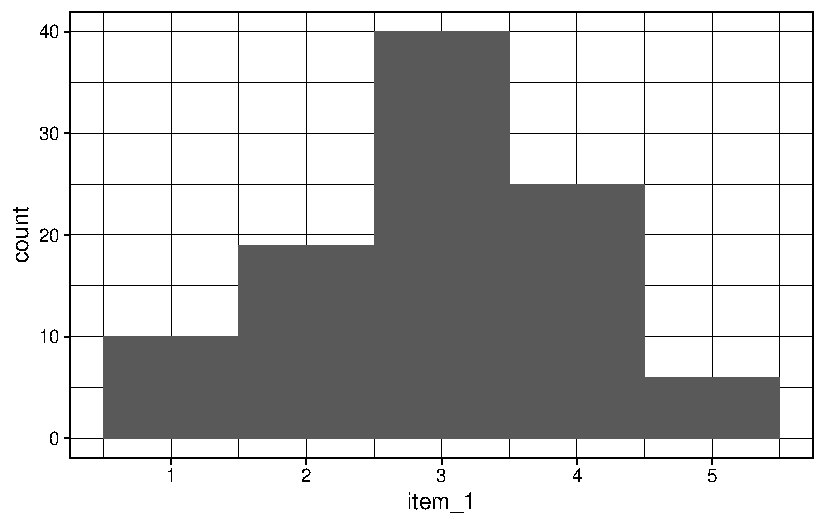
\includegraphics[keepaspectratio]{chapters/reshaping_and_pivots_files/figure-pdf/unnamed-chunk-5-1.pdf}}

\begin{Shaded}
\begin{Highlighting}[]
\FunctionTok{ggplot}\NormalTok{(data\_wide\_likert, }\FunctionTok{aes}\NormalTok{(}\AttributeTok{x =}\NormalTok{ item\_2)) }\SpecialCharTok{+}
  \FunctionTok{geom\_histogram}\NormalTok{(}\AttributeTok{binwidth =} \DecValTok{1}\NormalTok{, }\AttributeTok{boundary =} \SpecialCharTok{{-}}\FloatTok{0.5}\NormalTok{) }\SpecialCharTok{+}
  \FunctionTok{theme\_linedraw}\NormalTok{()}
\end{Highlighting}
\end{Shaded}

\pandocbounded{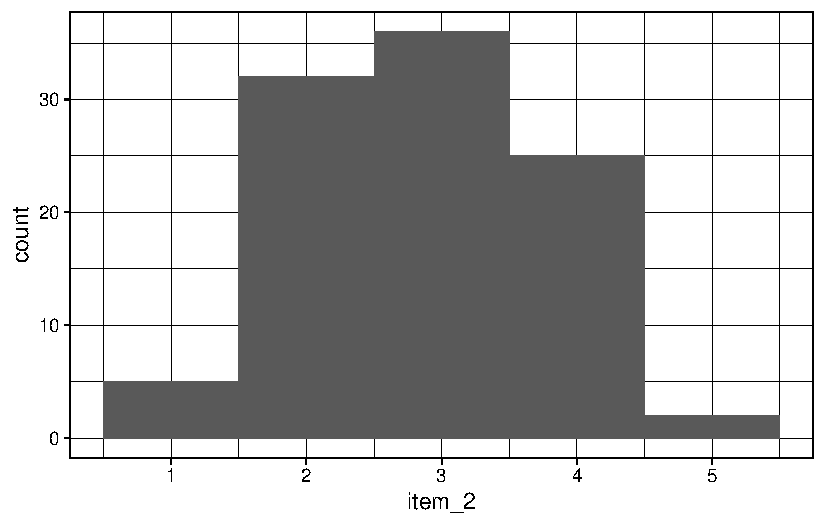
\includegraphics[keepaspectratio]{chapters/reshaping_and_pivots_files/figure-pdf/unnamed-chunk-5-2.pdf}}

\begin{Shaded}
\begin{Highlighting}[]
\FunctionTok{ggplot}\NormalTok{(data\_wide\_likert, }\FunctionTok{aes}\NormalTok{(}\AttributeTok{x =}\NormalTok{ item\_3)) }\SpecialCharTok{+}
  \FunctionTok{geom\_histogram}\NormalTok{(}\AttributeTok{binwidth =} \DecValTok{1}\NormalTok{, }\AttributeTok{boundary =} \SpecialCharTok{{-}}\FloatTok{0.5}\NormalTok{) }\SpecialCharTok{+}
  \FunctionTok{theme\_linedraw}\NormalTok{()}
\end{Highlighting}
\end{Shaded}

\pandocbounded{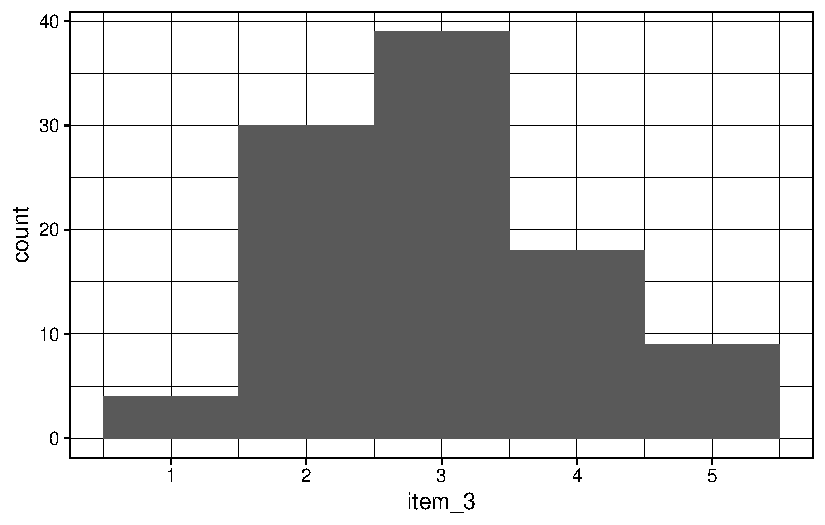
\includegraphics[keepaspectratio]{chapters/reshaping_and_pivots_files/figure-pdf/unnamed-chunk-5-3.pdf}}

\begin{Shaded}
\begin{Highlighting}[]
\FunctionTok{ggplot}\NormalTok{(data\_wide\_likert, }\FunctionTok{aes}\NormalTok{(}\AttributeTok{x =}\NormalTok{ item\_4)) }\SpecialCharTok{+}
  \FunctionTok{geom\_histogram}\NormalTok{(}\AttributeTok{binwidth =} \DecValTok{1}\NormalTok{, }\AttributeTok{boundary =} \SpecialCharTok{{-}}\FloatTok{0.5}\NormalTok{) }\SpecialCharTok{+}
  \FunctionTok{theme\_linedraw}\NormalTok{()}
\end{Highlighting}
\end{Shaded}

\pandocbounded{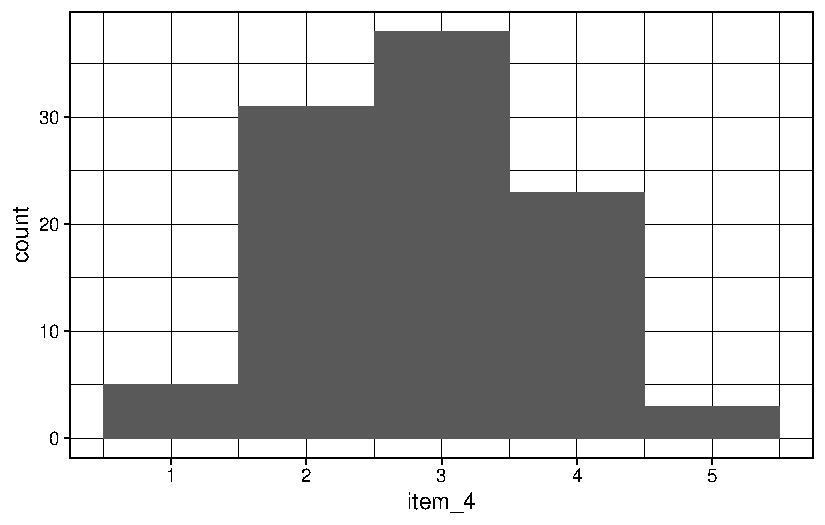
\includegraphics[keepaspectratio]{chapters/reshaping_and_pivots_files/figure-pdf/unnamed-chunk-5-4.pdf}}

\begin{Shaded}
\begin{Highlighting}[]
\FunctionTok{ggplot}\NormalTok{(data\_wide\_likert, }\FunctionTok{aes}\NormalTok{(}\AttributeTok{x =}\NormalTok{ item\_5)) }\SpecialCharTok{+}
  \FunctionTok{geom\_histogram}\NormalTok{(}\AttributeTok{binwidth =} \DecValTok{1}\NormalTok{, }\AttributeTok{boundary =} \SpecialCharTok{{-}}\FloatTok{0.5}\NormalTok{) }\SpecialCharTok{+}
  \FunctionTok{theme\_linedraw}\NormalTok{()}
\end{Highlighting}
\end{Shaded}

\pandocbounded{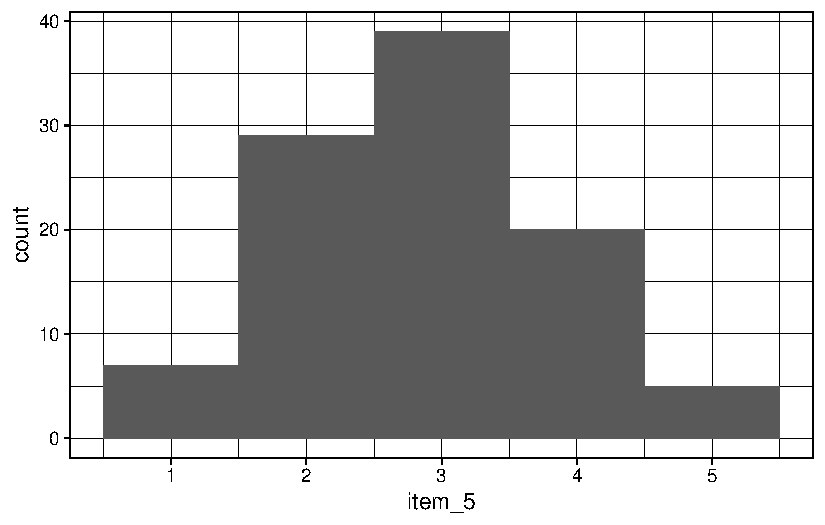
\includegraphics[keepaspectratio]{chapters/reshaping_and_pivots_files/figure-pdf/unnamed-chunk-5-5.pdf}}

\begin{itemize}
\tightlist
\item
  These plots repeat the mortal coding sin of repeating ourselves. If we
  reshaped the data to `long' format we could use just one ggplot() call
  that includes facet\_wrap().
\end{itemize}

\subsection{Reshape}\label{reshape}

Using \texttt{pivot\_longer()}.

\begin{Shaded}
\begin{Highlighting}[]
\CommentTok{\# positive selection}
\NormalTok{data\_long }\OtherTok{\textless{}{-}}\NormalTok{ data\_wide\_likert }\SpecialCharTok{\%\textgreater{}\%}
  \FunctionTok{pivot\_longer}\NormalTok{(}\AttributeTok{cols =} \FunctionTok{starts\_with}\NormalTok{(}\StringTok{"item\_"}\NormalTok{),}
               \AttributeTok{names\_to =} \StringTok{"item"}\NormalTok{,}
               \AttributeTok{values\_to =} \StringTok{"response"}\NormalTok{)}

\CommentTok{\# positive selection using a different tidy select function}
\NormalTok{data\_long }\OtherTok{\textless{}{-}}\NormalTok{ data\_wide\_likert }\SpecialCharTok{\%\textgreater{}\%}
  \FunctionTok{pivot\_longer}\NormalTok{(}\AttributeTok{cols =} \FunctionTok{contains}\NormalTok{(}\StringTok{"item\_"}\NormalTok{),}
               \AttributeTok{names\_to =} \StringTok{"item"}\NormalTok{,}
               \AttributeTok{values\_to =} \StringTok{"response"}\NormalTok{)}

\CommentTok{\# negative selection}
\NormalTok{data\_long }\OtherTok{\textless{}{-}}\NormalTok{ data\_wide\_likert }\SpecialCharTok{\%\textgreater{}\%}
  \FunctionTok{pivot\_longer}\NormalTok{(}\AttributeTok{cols =} \SpecialCharTok{{-}}\NormalTok{id,}
               \AttributeTok{names\_to =} \StringTok{"item"}\NormalTok{,}
               \AttributeTok{values\_to =} \StringTok{"response"}\NormalTok{) }\SpecialCharTok{|\textgreater{}}
  \FunctionTok{mutate}\NormalTok{(}\AttributeTok{item =}\NormalTok{ stringr}\SpecialCharTok{::}\FunctionTok{str\_remove}\NormalTok{(item, }\StringTok{"item\_"}\NormalTok{))}

\FunctionTok{ggplot}\NormalTok{(data\_long, }\FunctionTok{aes}\NormalTok{(}\AttributeTok{x =}\NormalTok{ response)) }\SpecialCharTok{+}
  \FunctionTok{geom\_histogram}\NormalTok{(}\AttributeTok{binwidth =} \DecValTok{1}\NormalTok{, }\AttributeTok{boundary =} \SpecialCharTok{{-}}\FloatTok{0.5}\NormalTok{) }\SpecialCharTok{+}
  \FunctionTok{theme\_linedraw}\NormalTok{() }\SpecialCharTok{+}
  \FunctionTok{facet\_wrap}\NormalTok{(}\SpecialCharTok{\textasciitilde{}}\NormalTok{ item)}
\end{Highlighting}
\end{Shaded}

\pandocbounded{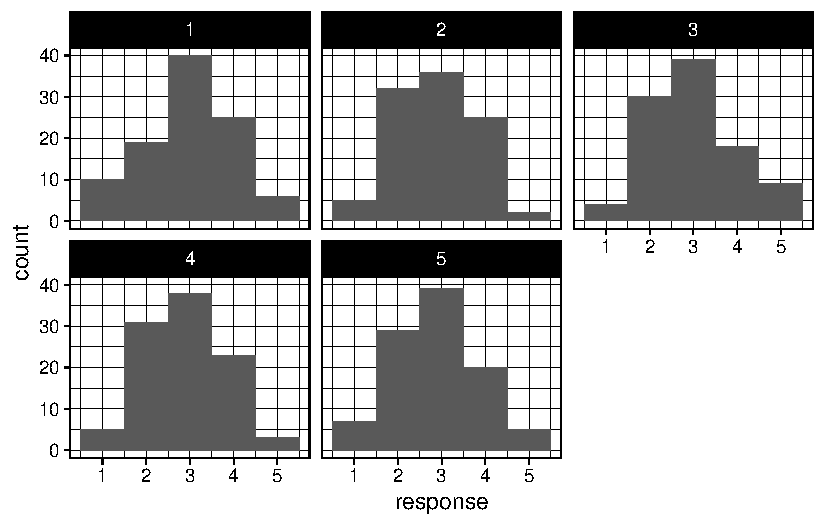
\includegraphics[keepaspectratio]{chapters/reshaping_and_pivots_files/figure-pdf/unnamed-chunk-6-1.pdf}}

\begin{itemize}
\tightlist
\item
  What other ways could you specify this pivot\_longer call's arguments?
\item
  \texttt{facet\_wrap()} is to \{ggplot\} as \texttt{group\_by()} is to
  \{dplyr\}
\end{itemize}

\subsubsection{Calculate sum scores}\label{calculate-sum-scores}

\begin{Shaded}
\begin{Highlighting}[]
\NormalTok{temp }\OtherTok{\textless{}{-}}\NormalTok{ data\_wide\_likert }\SpecialCharTok{|\textgreater{}}
  \FunctionTok{group\_by}\NormalTok{(id) }\SpecialCharTok{|\textgreater{}}
  \FunctionTok{mutate}\NormalTok{(}\AttributeTok{sum\_score =}\NormalTok{ item\_1 }\SpecialCharTok{+}\NormalTok{ item\_2 }\SpecialCharTok{+}\NormalTok{ item\_3 }\SpecialCharTok{+}\NormalTok{ item\_4 }\SpecialCharTok{+}\NormalTok{ item\_5)}
  \CommentTok{\#mutate(sum\_score = rowSums(item\_1, item\_2, item\_3, item\_4, item\_5))}
\end{Highlighting}
\end{Shaded}

\begin{itemize}
\tightlist
\item
  row math is much faster than column math in R!
\end{itemize}

\begin{Shaded}
\begin{Highlighting}[]
\NormalTok{sum\_scores }\OtherTok{\textless{}{-}}\NormalTok{ data\_long }\SpecialCharTok{\%\textgreater{}\%}
  \FunctionTok{group\_by}\NormalTok{(id) }\SpecialCharTok{\%\textgreater{}\%}
  \FunctionTok{summarise}\NormalTok{(}\AttributeTok{sum\_score =} \FunctionTok{sum}\NormalTok{(response))}


\FunctionTok{ggplot}\NormalTok{(sum\_scores, }\FunctionTok{aes}\NormalTok{(}\AttributeTok{x =}\NormalTok{ sum\_score)) }\SpecialCharTok{+}
  \FunctionTok{geom\_histogram}\NormalTok{(}\AttributeTok{binwidth =} \DecValTok{1}\NormalTok{, }\AttributeTok{boundary =} \SpecialCharTok{{-}}\FloatTok{0.5}\NormalTok{) }\SpecialCharTok{+}
  \FunctionTok{scale\_x\_continuous}\NormalTok{(}\AttributeTok{breaks =} \FunctionTok{breaks\_pretty}\NormalTok{(}\AttributeTok{n =} \DecValTok{10}\NormalTok{)) }\SpecialCharTok{+}
  \FunctionTok{theme\_linedraw}\NormalTok{()}
\end{Highlighting}
\end{Shaded}

\pandocbounded{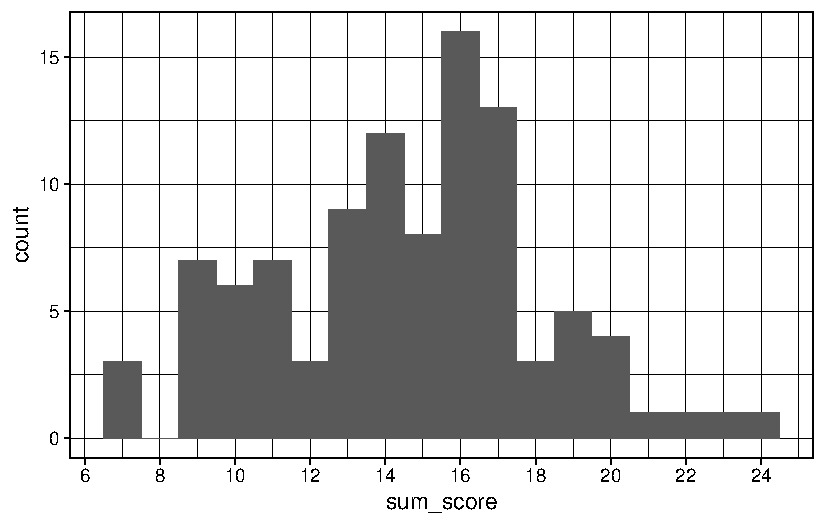
\includegraphics[keepaspectratio]{chapters/reshaping_and_pivots_files/figure-pdf/unnamed-chunk-8-1.pdf}}

\subsection{Convert this long data back to
wide}\label{convert-this-long-data-back-to-wide}

Just to know how to do it.

\begin{Shaded}
\begin{Highlighting}[]
\NormalTok{data\_wide\_again }\OtherTok{\textless{}{-}}\NormalTok{ data\_long }\SpecialCharTok{\%\textgreater{}\%}
  \FunctionTok{pivot\_wider}\NormalTok{(}\AttributeTok{names\_from =}\NormalTok{ item,}
              \AttributeTok{values\_from =}\NormalTok{ response,}
              \AttributeTok{names\_prefix =} \StringTok{"item\_"}\NormalTok{)}
\end{Highlighting}
\end{Shaded}

\subsection{Combine item and sum scores in one data
frame}\label{combine-item-and-sum-scores-in-one-data-frame}

\begin{Shaded}
\begin{Highlighting}[]
\NormalTok{data\_item\_and\_sum\_scores }\OtherTok{\textless{}{-}}\NormalTok{ data\_wide\_again }\SpecialCharTok{\%\textgreater{}\%}
  \FunctionTok{left\_join}\NormalTok{(sum\_scores, }\AttributeTok{by =} \StringTok{"id"}\NormalTok{)}

\CommentTok{\# why joins are needed over bind\_cols }
\CommentTok{\# wrong \textless{}{-} bind\_cols(data\_wide\_again, sum\_scores |\textgreater{} select({-}id))}
\end{Highlighting}
\end{Shaded}

\section{New facet plot with items and sum
score}\label{new-facet-plot-with-items-and-sum-score}

\begin{Shaded}
\begin{Highlighting}[]
\NormalTok{data\_long\_with\_sum\_score }\OtherTok{\textless{}{-}}\NormalTok{ data\_item\_and\_sum\_scores }\SpecialCharTok{\%\textgreater{}\%}
  \FunctionTok{pivot\_longer}\NormalTok{(}\AttributeTok{cols =} \SpecialCharTok{{-}}\NormalTok{id,}
               \AttributeTok{names\_to =} \StringTok{"item"}\NormalTok{,}
               \AttributeTok{values\_to =} \StringTok{"response"}\NormalTok{)}

\FunctionTok{ggplot}\NormalTok{(data\_long\_with\_sum\_score, }\FunctionTok{aes}\NormalTok{(}\AttributeTok{x =}\NormalTok{ response)) }\SpecialCharTok{+}
  \FunctionTok{geom\_histogram}\NormalTok{(}\AttributeTok{binwidth =} \DecValTok{1}\NormalTok{, }\AttributeTok{boundary =} \SpecialCharTok{{-}}\FloatTok{0.5}\NormalTok{) }\SpecialCharTok{+}
  \FunctionTok{theme\_linedraw}\NormalTok{() }\SpecialCharTok{+}
  \FunctionTok{facet\_wrap}\NormalTok{(}\SpecialCharTok{\textasciitilde{}}\NormalTok{ item, }\AttributeTok{scales =} \StringTok{"free"}\NormalTok{)}
\end{Highlighting}
\end{Shaded}

\pandocbounded{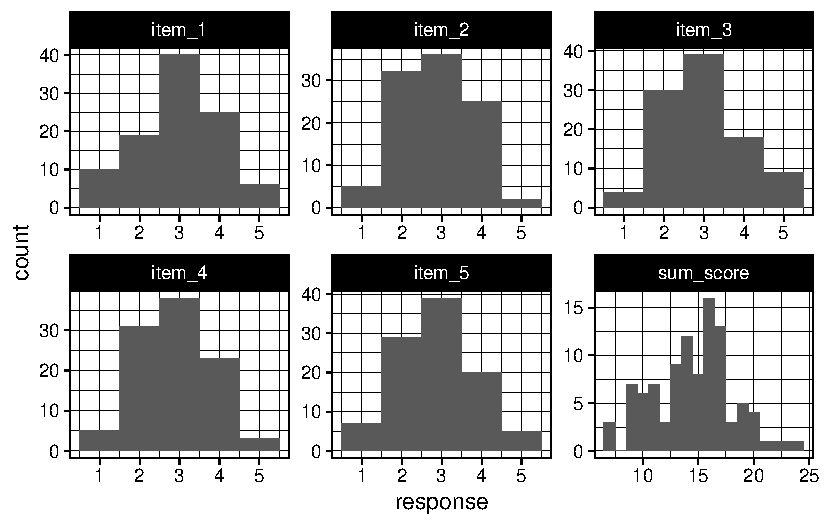
\includegraphics[keepaspectratio]{chapters/reshaping_and_pivots_files/figure-pdf/unnamed-chunk-11-1.pdf}}

\section{Practice}\label{practice}

Wrangle the demographics data included in this exercise more efficiently
by reshaping it into wide format. Before, we used filter() to wrangle
the age and gender data separately.

\begin{Shaded}
\begin{Highlighting}[]
\NormalTok{dat }\OtherTok{\textless{}{-}} \FunctionTok{read\_csv}\NormalTok{(}\StringTok{"../data/raw/data\_demographics\_raw.csv"}\NormalTok{)}
\end{Highlighting}
\end{Shaded}

\begin{verbatim}
Rows: 200 Columns: 17
-- Column specification --------------------------------------------------------
Delimiter: ","
chr   (4): build, blockcode, trialcode, response
dbl  (11): group, subject, session, blocknum, trialnum, pretrialpause, postt...
date  (1): date
time  (1): time

i Use `spec()` to retrieve the full column specification for this data.
i Specify the column types or set `show_col_types = FALSE` to quiet this message.
\end{verbatim}

\bookmarksetup{startatroot}

\chapter{Joins}\label{joins}

\section{Dependencies}\label{dependencies-3}

\begin{Shaded}
\begin{Highlighting}[]
\FunctionTok{library}\NormalTok{(dplyr)}
\end{Highlighting}
\end{Shaded}

\begin{verbatim}

Attaching package: 'dplyr'
\end{verbatim}

\begin{verbatim}
The following objects are masked from 'package:stats':

    filter, lag
\end{verbatim}

\begin{verbatim}
The following objects are masked from 'package:base':

    intersect, setdiff, setequal, union
\end{verbatim}

\begin{Shaded}
\begin{Highlighting}[]
\FunctionTok{library}\NormalTok{(readr)}
\end{Highlighting}
\end{Shaded}

\section{Get data}\label{get-data}

\begin{Shaded}
\begin{Highlighting}[]
\NormalTok{data\_unique\_id\_subset }\OtherTok{\textless{}{-}} \FunctionTok{read\_csv}\NormalTok{(}\StringTok{"../data/raw/data\_unique\_id\_subset.csv"}\NormalTok{)}
\end{Highlighting}
\end{Shaded}

\begin{verbatim}
Rows: 92 Columns: 1
-- Column specification --------------------------------------------------------
Delimiter: ","
dbl (1): unique_id

i Use `spec()` to retrieve the full column specification for this data.
i Specify the column types or set `show_col_types = FALSE` to quiet this message.
\end{verbatim}

\begin{Shaded}
\begin{Highlighting}[]
\NormalTok{data\_age\_gender\_subset }\OtherTok{\textless{}{-}} \FunctionTok{read\_csv}\NormalTok{(}\StringTok{"../data/raw/data\_age\_gender\_subset.csv"}\NormalTok{)}
\end{Highlighting}
\end{Shaded}

\begin{verbatim}
Rows: 90 Columns: 3
-- Column specification --------------------------------------------------------
Delimiter: ","
chr (1): gender
dbl (2): unique_id, age

i Use `spec()` to retrieve the full column specification for this data.
i Specify the column types or set `show_col_types = FALSE` to quiet this message.
\end{verbatim}

\begin{Shaded}
\begin{Highlighting}[]
\NormalTok{data\_amp\_summary\_subset }\OtherTok{\textless{}{-}} \FunctionTok{read\_csv}\NormalTok{(}\StringTok{"../data/raw/data\_amp\_summary\_subset.csv"}\NormalTok{)}
\end{Highlighting}
\end{Shaded}

\begin{verbatim}
Rows: 31 Columns: 2
-- Column specification --------------------------------------------------------
Delimiter: ","
dbl (2): unique_id, mean_reaction_time_behavioral_task

i Use `spec()` to retrieve the full column specification for this data.
i Specify the column types or set `show_col_types = FALSE` to quiet this message.
\end{verbatim}

\begin{Shaded}
\begin{Highlighting}[]
\NormalTok{data\_selfreport\_summary\_subset }\OtherTok{\textless{}{-}} \FunctionTok{read\_csv}\NormalTok{(}\StringTok{"../data/raw/data\_selfreport\_summary\_subset.csv"}\NormalTok{)}
\end{Highlighting}
\end{Shaded}

\begin{verbatim}
Rows: 76 Columns: 2
-- Column specification --------------------------------------------------------
Delimiter: ","
dbl (2): unique_id, mean_self_report

i Use `spec()` to retrieve the full column specification for this data.
i Specify the column types or set `show_col_types = FALSE` to quiet this message.
\end{verbatim}

\begin{Shaded}
\begin{Highlighting}[]
\FunctionTok{nrow}\NormalTok{(data\_unique\_id\_subset)}
\end{Highlighting}
\end{Shaded}

\begin{verbatim}
[1] 92
\end{verbatim}

\begin{Shaded}
\begin{Highlighting}[]
\FunctionTok{nrow}\NormalTok{(data\_age\_gender\_subset)}
\end{Highlighting}
\end{Shaded}

\begin{verbatim}
[1] 90
\end{verbatim}

\begin{Shaded}
\begin{Highlighting}[]
\FunctionTok{nrow}\NormalTok{(data\_amp\_summary\_subset)}
\end{Highlighting}
\end{Shaded}

\begin{verbatim}
[1] 31
\end{verbatim}

\begin{Shaded}
\begin{Highlighting}[]
\FunctionTok{nrow}\NormalTok{(data\_selfreport\_summary\_subset)}
\end{Highlighting}
\end{Shaded}

\begin{verbatim}
[1] 76
\end{verbatim}

\section{Practicing joins}\label{practicing-joins}

Using the data frames below and functions from the \_join family, write
code to do the following joins.

\subsection{Practice 1}\label{practice-1}

create `data\_combined' by joining data\_amp\_summary\_subset and
data\_age\_gender\_subset so that unique\_ids in either data frame are
retained. which join is this? implement it.

\begin{Shaded}
\begin{Highlighting}[]
\CommentTok{\# data\_combined \textless{}{-} }
\end{Highlighting}
\end{Shaded}

\subsection{Practice 2}\label{practice-2}

create `data\_self\_reports\_and\_their\_amp\_data' by joining
data\_selfreport\_summary\_subset and data\_amp\_summary\_subset so that
all participants have self-report data, + AMP data if available. which
join is this? implement it.

\begin{Shaded}
\begin{Highlighting}[]
\CommentTok{\# data\_self\_reports\_and\_their\_amp\_data \textless{}{-} }
\end{Highlighting}
\end{Shaded}

\subsection{Practice 3}\label{practice-3}

do the opposite: create `data\_amp\_data\_and\_their\_self\_reports' by
joining data\_amp\_summary\_subset and data\_selfreport\_summary\_subset
so that all participants have AMP data, + self-report data if available.
which join is this? implement it.

\begin{Shaded}
\begin{Highlighting}[]
\CommentTok{\# data\_amp\_data\_and\_their\_self\_reports \textless{}{-} }
\end{Highlighting}
\end{Shaded}

\subsection{Practice 4}\label{practice-4}

create data\_combined\_2 by joining `data\_combined' and
data\_selfreport\_summary\_subset only unique\_ids already present in
data\_combined are retained. which join is this? implement it.

\begin{Shaded}
\begin{Highlighting}[]
\CommentTok{\# data\_combined\_2 \textless{}{-} }
\end{Highlighting}
\end{Shaded}

\subsection{Practice 5}\label{practice-5}

create `data\_missing\_ids' which should list the unique\_ids are
missing from data\_unique\_id\_subset but are present in at least one of
data\_age\_gender\_subset, data\_amp\_summary\_subset, and
data\_selfreport\_summary\_subset. This will require two different
joins. Which? Implement them.

\begin{Shaded}
\begin{Highlighting}[]
\CommentTok{\# data\_missing\_ids \textless{}{-} }
\end{Highlighting}
\end{Shaded}

\bookmarksetup{startatroot}

\chapter{Reporting}\label{reporting}

\section{Dependencies}\label{dependencies-4}

\begin{Shaded}
\begin{Highlighting}[]
\FunctionTok{library}\NormalTok{(dplyr)}
\end{Highlighting}
\end{Shaded}

\begin{verbatim}

Attaching package: 'dplyr'
\end{verbatim}

\begin{verbatim}
The following objects are masked from 'package:stats':

    filter, lag
\end{verbatim}

\begin{verbatim}
The following objects are masked from 'package:base':

    intersect, setdiff, setequal, union
\end{verbatim}

\begin{Shaded}
\begin{Highlighting}[]
\FunctionTok{library}\NormalTok{(readr)}
\FunctionTok{library}\NormalTok{(report) }\CommentTok{\# part of \{easystats\}}
\FunctionTok{library}\NormalTok{(see) }\CommentTok{\# part of \{easystats\}}
\FunctionTok{library}\NormalTok{(parameters) }\CommentTok{\# part of \{easystats\}}
\FunctionTok{library}\NormalTok{(correlation) }\CommentTok{\# part of \{easystats\}}
\FunctionTok{library}\NormalTok{(effectsize) }\CommentTok{\# part of \{easystats\}}
\FunctionTok{library}\NormalTok{(performance) }\CommentTok{\# part of \{easystats\}}
\FunctionTok{library}\NormalTok{(janitor)}
\end{Highlighting}
\end{Shaded}

\begin{verbatim}

Attaching package: 'janitor'
\end{verbatim}

\begin{verbatim}
The following objects are masked from 'package:stats':

    chisq.test, fisher.test
\end{verbatim}

\begin{Shaded}
\begin{Highlighting}[]
\FunctionTok{library}\NormalTok{(lme4)}
\end{Highlighting}
\end{Shaded}

\begin{verbatim}
Loading required package: Matrix
\end{verbatim}

\begin{Shaded}
\begin{Highlighting}[]
\FunctionTok{library}\NormalTok{(knitr)}
\FunctionTok{library}\NormalTok{(kableExtra)}
\end{Highlighting}
\end{Shaded}

\begin{verbatim}

Attaching package: 'kableExtra'
\end{verbatim}

\begin{verbatim}
The following object is masked from 'package:dplyr':

    group_rows
\end{verbatim}

\section{Inference tests}\label{inference-tests}

\subsection{Regressions}\label{regressions}

\begin{Shaded}
\begin{Highlighting}[]
\CommentTok{\# fit model}
\NormalTok{model }\OtherTok{\textless{}{-}} \FunctionTok{lm}\NormalTok{(wt }\SpecialCharTok{\textasciitilde{}} \DecValTok{1} \SpecialCharTok{+}\NormalTok{ am }\SpecialCharTok{+}\NormalTok{ mpg, }\AttributeTok{data =}\NormalTok{ mtcars)}

\CommentTok{\# report {-} text output (nb omits intercept!)}
\FunctionTok{report}\NormalTok{(model)}
\end{Highlighting}
\end{Shaded}

\begin{verbatim}
We fitted a linear model (estimated using OLS) to predict wt with am and mpg
(formula: wt ~ 1 + am + mpg). The model explains a statistically significant
and substantial proportion of variance (R2 = 0.80, F(2, 29) = 57.66, p < .001,
adj. R2 = 0.79). The model's intercept, corresponding to am = 0 and mpg = 0, is
at 5.74 (95% CI [5.11, 6.36], t(29) = 18.64, p < .001). Within this model:

  - The effect of am is statistically significant and negative (beta = -0.53, 95%
CI [-0.94, -0.11], t(29) = -2.58, p = 0.015; Std. beta = -0.27, 95% CI [-0.48,
-0.06])
  - The effect of mpg is statistically significant and negative (beta = -0.11,
95% CI [-0.15, -0.08], t(29) = -6.79, p < .001; Std. beta = -0.71, 95% CI
[-0.92, -0.49])

Standardized parameters were obtained by fitting the model on a standardized
version of the dataset. 95% Confidence Intervals (CIs) and p-values were
computed using a Wald t-distribution approximation.
\end{verbatim}

\begin{Shaded}
\begin{Highlighting}[]
\CommentTok{\# each parameter (including intercept)}
\FunctionTok{report\_parameters}\NormalTok{(model)}
\end{Highlighting}
\end{Shaded}

\begin{verbatim}
  - The intercept is statistically significant and positive (beta = 5.74, 95% CI [5.11, 6.36], t(29) = 18.64, p < .001; Std. beta = 1.10e-16, 95% CI [-0.17, 0.17])
  - The effect of am is statistically significant and negative (beta = -0.53, 95% CI [-0.94, -0.11], t(29) = -2.58, p = 0.015; Std. beta = -0.27, 95% CI [-0.48, -0.06])
  - The effect of mpg is statistically significant and negative (beta = -0.11, 95% CI [-0.15, -0.08], t(29) = -6.79, p < .001; Std. beta = -0.71, 95% CI [-0.92, -0.49])
\end{verbatim}

\begin{Shaded}
\begin{Highlighting}[]
\CommentTok{\# just parameters in text format}
\FunctionTok{report\_statistics}\NormalTok{(model)}
\end{Highlighting}
\end{Shaded}

\begin{verbatim}
beta = 5.74, 95% CI [5.11, 6.36], t(29) = 18.64, p < .001; Std. beta = 1.10e-16, 95% CI [-0.17, 0.17]
beta = -0.53, 95% CI [-0.94, -0.11], t(29) = -2.58, p = 0.015; Std. beta = -0.27, 95% CI [-0.48, -0.06]
beta = -0.11, 95% CI [-0.15, -0.08], t(29) = -6.79, p < .001; Std. beta = -0.71, 95% CI [-0.92, -0.49]
\end{verbatim}

\begin{Shaded}
\begin{Highlighting}[]
\CommentTok{\# just parameters in table format}
\FunctionTok{parameters}\NormalTok{(model)}
\end{Highlighting}
\end{Shaded}

\begin{verbatim}
Parameter   | Coefficient |   SE |         95% CI | t(29) |      p
------------------------------------------------------------------
(Intercept) |        5.74 | 0.31 | [ 5.11,  6.36] | 18.64 | < .001
am          |       -0.53 | 0.20 | [-0.94, -0.11] | -2.58 | 0.015 
mpg         |       -0.11 | 0.02 | [-0.15, -0.08] | -6.79 | < .001
\end{verbatim}

\begin{verbatim}

Uncertainty intervals (equal-tailed) and p-values (two-tailed) computed
  using a Wald t-distribution approximation.
\end{verbatim}

\begin{Shaded}
\begin{Highlighting}[]
\CommentTok{\# just parameters in table html format }
\FunctionTok{parameters}\NormalTok{(model) }\SpecialCharTok{|\textgreater{}}
  \FunctionTok{mutate}\NormalTok{(}\AttributeTok{p =}\NormalTok{ insight}\SpecialCharTok{::}\FunctionTok{format\_p}\NormalTok{(p)) }\SpecialCharTok{|\textgreater{}}
  \FunctionTok{mutate\_if}\NormalTok{(is.numeric, round\_half\_up, }\AttributeTok{digits =} \DecValTok{2}\NormalTok{) }\SpecialCharTok{|\textgreater{}}
  \FunctionTok{kable}\NormalTok{() }\SpecialCharTok{|\textgreater{}}
  \FunctionTok{kable\_classic}\NormalTok{(}\AttributeTok{full\_width =} \ConstantTok{FALSE}\NormalTok{)}
\end{Highlighting}
\end{Shaded}

\begin{longtable*}[t]{lrrrrrrrl}
\toprule
Parameter & Coefficient & SE & CI & CI\_low & CI\_high & t & df\_error & p\\
\midrule
(Intercept) & 5.74 & 0.31 & 0.95 & 5.11 & 6.36 & 18.64 & 29 & p < .001\\
am & -0.53 & 0.20 & 0.95 & -0.94 & -0.11 & -2.58 & 29 & p = 0.015\\
mpg & -0.11 & 0.02 & 0.95 & -0.15 & -0.08 & -6.79 & 29 & p < .001\\
\bottomrule
\end{longtable*}

\begin{Shaded}
\begin{Highlighting}[]
\CommentTok{\# what if i just want some of these cols?}
\FunctionTok{parameters}\NormalTok{(model) }\SpecialCharTok{|\textgreater{}}
  \FunctionTok{as.data.frame}\NormalTok{() }\SpecialCharTok{|\textgreater{}}
  \FunctionTok{mutate}\NormalTok{(}\AttributeTok{p =}\NormalTok{ insight}\SpecialCharTok{::}\FunctionTok{format\_p}\NormalTok{(p)) }\SpecialCharTok{|\textgreater{}}
  \FunctionTok{select}\NormalTok{(}\AttributeTok{r =}\NormalTok{ Coefficient, }\AttributeTok{ci\_lower =}\NormalTok{ CI\_low, }\AttributeTok{ci\_upper =}\NormalTok{ CI\_high, p) }\SpecialCharTok{|\textgreater{}}
  \FunctionTok{mutate\_if}\NormalTok{(is.numeric, round\_half\_up, }\AttributeTok{digits =} \DecValTok{2}\NormalTok{)}
\end{Highlighting}
\end{Shaded}

\begin{verbatim}
      r ci_lower ci_upper         p
1  5.74     5.11     6.36  p < .001
2 -0.53    -0.94    -0.11 p = 0.015
3 -0.11    -0.15    -0.08  p < .001
\end{verbatim}

\begin{Shaded}
\begin{Highlighting}[]
\CommentTok{\# table in markdown format}
\FunctionTok{report\_table}\NormalTok{(model)}
\end{Highlighting}
\end{Shaded}

\begin{verbatim}
Parameter   | Coefficient |         95% CI | t(29) |      p | Std. Coef.
------------------------------------------------------------------------
(Intercept) |        5.74 | [ 5.11,  6.36] | 18.64 | < .001 |   1.10e-16
am          |       -0.53 | [-0.94, -0.11] | -2.58 | 0.015  |      -0.27
mpg         |       -0.11 | [-0.15, -0.08] | -6.79 | < .001 |      -0.71
            |             |                |       |        |           
AIC         |             |                |       |        |           
AICc        |             |                |       |        |           
BIC         |             |                |       |        |           
R2          |             |                |       |        |           
R2 (adj.)   |             |                |       |        |           
Sigma       |             |                |       |        |           

Parameter   | Std. Coef. 95% CI |   Fit
---------------------------------------
(Intercept) |    [-0.17,  0.17] |      
am          |    [-0.48, -0.06] |      
mpg         |    [-0.92, -0.49] |      
            |                   |      
AIC         |                   | 45.05
AICc        |                   | 46.53
BIC         |                   | 50.91
R2          |                   |  0.80
R2 (adj.)   |                   |  0.79
Sigma       |                   |  0.45
\end{verbatim}

\begin{Shaded}
\begin{Highlighting}[]
\CommentTok{\# table in html format {-} needs to be rounded manually}
\FunctionTok{report\_table}\NormalTok{(model) }\SpecialCharTok{|\textgreater{}}
  \FunctionTok{mutate}\NormalTok{(}\AttributeTok{p =}\NormalTok{ insight}\SpecialCharTok{::}\FunctionTok{format\_p}\NormalTok{(p)) }\SpecialCharTok{|\textgreater{}}
  \FunctionTok{mutate\_if}\NormalTok{(is.numeric, round\_half\_up, }\AttributeTok{digits =} \DecValTok{2}\NormalTok{) }\SpecialCharTok{|\textgreater{}}
  \FunctionTok{kable}\NormalTok{() }\SpecialCharTok{|\textgreater{}}
  \FunctionTok{kable\_classic}\NormalTok{(}\AttributeTok{full\_width =} \ConstantTok{FALSE}\NormalTok{)}
\end{Highlighting}
\end{Shaded}

\begin{longtable*}[t]{llrrrrrrlrrrr}
\toprule
 & Parameter & Coefficient & CI & CI\_low & CI\_high & t & df\_error & p & Std\_Coefficient & Std\_Coefficient\_CI\_low & Std\_Coefficient\_CI\_high & Fit\\
\midrule
1 & (Intercept) & 5.74 & 0.95 & 5.11 & 6.36 & 18.64 & 29 & p < .001 & 0.00 & -0.17 & 0.17 & NA\\
2 & am & -0.53 & 0.95 & -0.94 & -0.11 & -2.58 & 29 & p = 0.015 & -0.27 & -0.48 & -0.06 & NA\\
3 & mpg & -0.11 & 0.95 & -0.15 & -0.08 & -6.79 & 29 & p < .001 & -0.71 & -0.92 & -0.49 & NA\\
4 & NA & NA & NA & NA & NA & NA & NA &  & NA & NA & NA & NA\\
5 & AIC & NA & NA & NA & NA & NA & NA &  & NA & NA & NA & 45.05\\
\addlinespace
6 & AICc & NA & NA & NA & NA & NA & NA &  & NA & NA & NA & 46.53\\
7 & BIC & NA & NA & NA & NA & NA & NA &  & NA & NA & NA & 50.91\\
8 & R2 & NA & NA & NA & NA & NA & NA &  & NA & NA & NA & 0.80\\
9 & R2 (adj.) & NA & NA & NA & NA & NA & NA &  & NA & NA & NA & 0.79\\
11 & Sigma & NA & NA & NA & NA & NA & NA &  & NA & NA & NA & 0.45\\
\bottomrule
\end{longtable*}

\begin{Shaded}
\begin{Highlighting}[]
\CommentTok{\# plot}
\FunctionTok{parameters}\NormalTok{(model) }\SpecialCharTok{|\textgreater{}}
  \FunctionTok{plot}\NormalTok{() }
\end{Highlighting}
\end{Shaded}

\pandocbounded{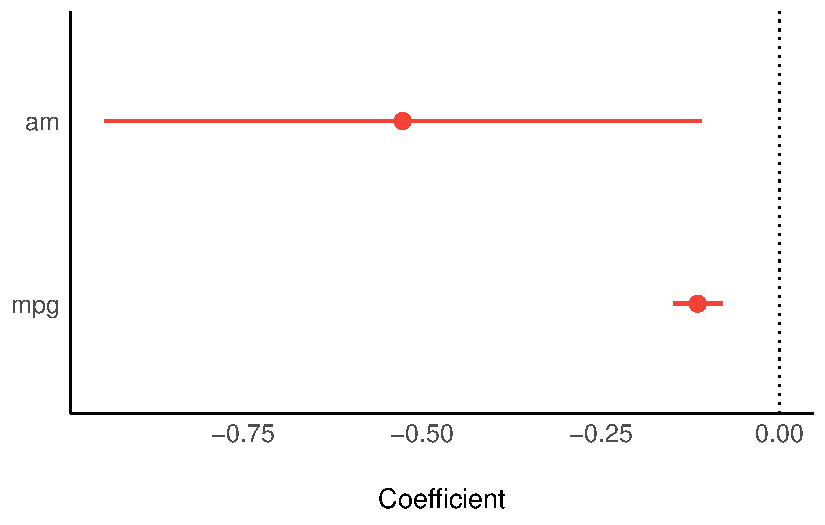
\includegraphics[keepaspectratio]{chapters/reporting_files/figure-pdf/unnamed-chunk-3-1.pdf}}

\subsection{Correlations}\label{correlations}

\subsubsection{Single correlation tests}\label{single-correlation-tests}

\begin{Shaded}
\begin{Highlighting}[]
\CommentTok{\# fit model}
\NormalTok{model }\OtherTok{\textless{}{-}} \FunctionTok{cor.test}\NormalTok{(mtcars}\SpecialCharTok{$}\NormalTok{mpg, mtcars}\SpecialCharTok{$}\NormalTok{wt)}

\CommentTok{\# report {-} text output }
\FunctionTok{report}\NormalTok{(model)}
\end{Highlighting}
\end{Shaded}

\begin{verbatim}
Effect sizes were labelled following Funder's (2019) recommendations.

The Pearson's product-moment correlation between mtcars$mpg and mtcars$wt is
negative, statistically significant, and very large (r = -0.87, 95% CI [-0.93,
-0.74], t(30) = -9.56, p < .001)
\end{verbatim}

\begin{Shaded}
\begin{Highlighting}[]
\CommentTok{\# table in html format {-} needs to be rounded manually}
\FunctionTok{report\_table}\NormalTok{(model) }\SpecialCharTok{|\textgreater{}}
  \FunctionTok{mutate}\NormalTok{(}\AttributeTok{p =}\NormalTok{ insight}\SpecialCharTok{::}\FunctionTok{format\_p}\NormalTok{(p)) }\SpecialCharTok{|\textgreater{}}
  \FunctionTok{mutate\_if}\NormalTok{(is.numeric, round\_half\_up, }\AttributeTok{digits =} \DecValTok{2}\NormalTok{) }\SpecialCharTok{|\textgreater{}}
  \FunctionTok{kable}\NormalTok{() }\SpecialCharTok{|\textgreater{}}
  \FunctionTok{kable\_classic}\NormalTok{(}\AttributeTok{full\_width =} \ConstantTok{FALSE}\NormalTok{)}
\end{Highlighting}
\end{Shaded}

\begin{longtable*}[t]{llrrrrrrlll}
\toprule
Parameter1 & Parameter2 & r & CI & CI\_low & CI\_high & t & df\_error & p & Method & Alternative\\
\midrule
mtcars\$mpg & mtcars\$wt & -0.87 & 0.95 & -0.93 & -0.74 & -9.56 & 30 & p < .001 & Pearson's product-moment correlation & two.sided\\
\bottomrule
\end{longtable*}

\subsubsection{Many}\label{many}

\begin{Shaded}
\begin{Highlighting}[]
\NormalTok{results }\OtherTok{\textless{}{-}} \FunctionTok{correlation}\NormalTok{(iris)}

\NormalTok{results}
\end{Highlighting}
\end{Shaded}

\begin{verbatim}
# Correlation Matrix (pearson-method)

Parameter1   |   Parameter2 |     r |         95% CI | t(148) |         p
-------------------------------------------------------------------------
Sepal.Length |  Sepal.Width | -0.12 | [-0.27,  0.04] |  -1.44 | 0.152    
Sepal.Length | Petal.Length |  0.87 | [ 0.83,  0.91] |  21.65 | < .001***
Sepal.Length |  Petal.Width |  0.82 | [ 0.76,  0.86] |  17.30 | < .001***
Sepal.Width  | Petal.Length | -0.43 | [-0.55, -0.29] |  -5.77 | < .001***
Sepal.Width  |  Petal.Width | -0.37 | [-0.50, -0.22] |  -4.79 | < .001***
Petal.Length |  Petal.Width |  0.96 | [ 0.95,  0.97] |  43.39 | < .001***

p-value adjustment method: Holm (1979)
Observations: 150
\end{verbatim}

\begin{Shaded}
\begin{Highlighting}[]
\NormalTok{results }\SpecialCharTok{\%\textgreater{}\%}
  \FunctionTok{summary}\NormalTok{(}\AttributeTok{redundant =} \ConstantTok{TRUE}\NormalTok{) }\SpecialCharTok{\%\textgreater{}\%}
  \FunctionTok{plot}\NormalTok{()}
\end{Highlighting}
\end{Shaded}

\pandocbounded{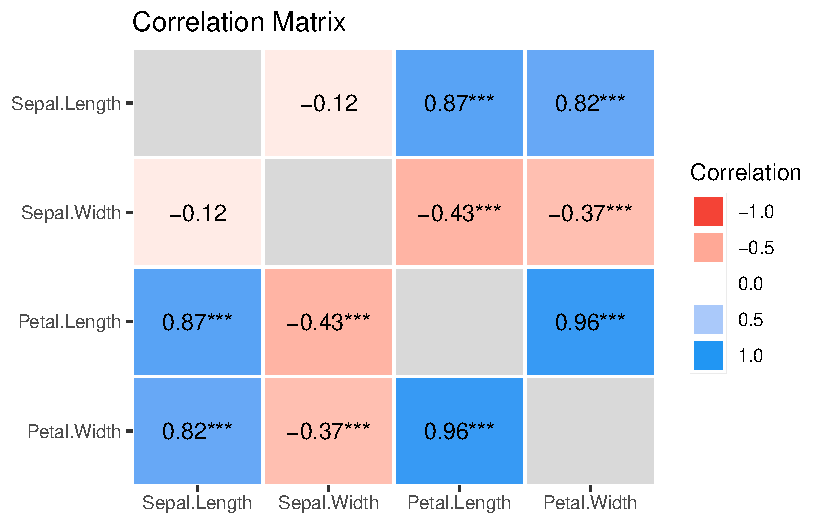
\includegraphics[keepaspectratio]{chapters/reporting_files/figure-pdf/unnamed-chunk-5-1.pdf}}

\subsubsection{By group}\label{by-group}

\begin{Shaded}
\begin{Highlighting}[]
\NormalTok{iris }\SpecialCharTok{\%\textgreater{}\%}
  \FunctionTok{select}\NormalTok{(Species, Sepal.Length, Sepal.Width, Petal.Width) }\SpecialCharTok{\%\textgreater{}\%}
  \FunctionTok{group\_by}\NormalTok{(Species) }\SpecialCharTok{\%\textgreater{}\%}
  \FunctionTok{correlation}\NormalTok{()}
\end{Highlighting}
\end{Shaded}

\begin{verbatim}
# Correlation Matrix (pearson-method)

Group      |   Parameter1 |  Parameter2 |    r |        95% CI | t(48) |         p
----------------------------------------------------------------------------------
setosa     | Sepal.Length | Sepal.Width | 0.74 | [ 0.59, 0.85] |  7.68 | < .001***
setosa     | Sepal.Length | Petal.Width | 0.28 | [ 0.00, 0.52] |  2.01 | 0.101    
setosa     |  Sepal.Width | Petal.Width | 0.23 | [-0.05, 0.48] |  1.66 | 0.104    
versicolor | Sepal.Length | Sepal.Width | 0.53 | [ 0.29, 0.70] |  4.28 | < .001***
versicolor | Sepal.Length | Petal.Width | 0.55 | [ 0.32, 0.72] |  4.52 | < .001***
versicolor |  Sepal.Width | Petal.Width | 0.66 | [ 0.47, 0.80] |  6.15 | < .001***
virginica  | Sepal.Length | Sepal.Width | 0.46 | [ 0.20, 0.65] |  3.56 | 0.002**  
virginica  | Sepal.Length | Petal.Width | 0.28 | [ 0.00, 0.52] |  2.03 | 0.048*   
virginica  |  Sepal.Width | Petal.Width | 0.54 | [ 0.31, 0.71] |  4.42 | < .001***

p-value adjustment method: Holm (1979)
Observations: 50
\end{verbatim}

\subsection{t-tests}\label{t-tests}

NB Cohen's d is approximated - better to calculate it separately and
accurately.

\begin{Shaded}
\begin{Highlighting}[]
\CommentTok{\# fit model}
\NormalTok{model }\OtherTok{\textless{}{-}} \FunctionTok{t.test}\NormalTok{(mpg }\SpecialCharTok{\textasciitilde{}}\NormalTok{ am, }\AttributeTok{data =}\NormalTok{ mtcars)}

\CommentTok{\# report {-} text output }
\FunctionTok{report}\NormalTok{(model)}
\end{Highlighting}
\end{Shaded}

\begin{verbatim}
In the report() function, for htest objects, you can try providing the
  data argument manually, e.g., report(x, data = data).
\end{verbatim}

\begin{verbatim}
Warning: Unable to retrieve data from htest object.
  Returning an approximate effect size using t_to_d().
\end{verbatim}

\begin{verbatim}
Effect sizes were labelled following Cohen's (1988) recommendations.

The Welch Two Sample t-test testing the difference of mpg by am (mean in group
0 = 17.15, mean in group 1 = 24.39) suggests that the effect is negative,
statistically significant, and large (difference = -7.24, 95% CI [-11.28,
-3.21], t(18.33) = -3.77, p = 0.001; Cohen's d = -1.76, 95% CI [-2.82, -0.67])
\end{verbatim}

\begin{Shaded}
\begin{Highlighting}[]
\CommentTok{\# table in html format {-} needs to be rounded manually}
\FunctionTok{report\_table}\NormalTok{(model) }\SpecialCharTok{|\textgreater{}}
  \FunctionTok{mutate}\NormalTok{(}\AttributeTok{p =}\NormalTok{ insight}\SpecialCharTok{::}\FunctionTok{format\_p}\NormalTok{(p)) }\SpecialCharTok{|\textgreater{}}
  \FunctionTok{mutate\_if}\NormalTok{(is.numeric, round\_half\_up, }\AttributeTok{digits =} \DecValTok{2}\NormalTok{) }\SpecialCharTok{|\textgreater{}}
  \FunctionTok{kable}\NormalTok{() }\SpecialCharTok{|\textgreater{}}
  \FunctionTok{kable\_classic}\NormalTok{(}\AttributeTok{full\_width =} \ConstantTok{FALSE}\NormalTok{)}
\end{Highlighting}
\end{Shaded}

\begin{verbatim}
In the report() function, for htest objects, you can try providing the
  data argument manually, e.g., report(x, data = data).
\end{verbatim}

\begin{verbatim}
Warning: Unable to retrieve data from htest object.
  Returning an approximate effect size using t_to_d().
\end{verbatim}

\begin{longtable*}[t]{llrrrrrrrrlllrrr}
\toprule
Parameter & Group & Mean\_Group1 & Mean\_Group2 & Difference & CI & CI\_low & CI\_high & t & df\_error & p & Method & Alternative & d & d\_CI\_low & d\_CI\_high\\
\midrule
mpg & am & 17.15 & 24.39 & -7.24 & 0.95 & -11.28 & -3.21 & -3.77 & 18.33 & p = 0.001 & Welch Two Sample t-test & two.sided & -1.76 & -2.82 & -0.67\\
\bottomrule
\end{longtable*}

\begin{Shaded}
\begin{Highlighting}[]
\CommentTok{\# estimate Cohen\textquotesingle{}s d directly from data}
\FunctionTok{cohens\_d}\NormalTok{(mpg }\SpecialCharTok{\textasciitilde{}}\NormalTok{ am, }\AttributeTok{data =}\NormalTok{ mtcars)}
\end{Highlighting}
\end{Shaded}

\begin{verbatim}
Cohen's d |         95% CI
--------------------------
-1.48     | [-2.27, -0.67]

- Estimated using pooled SD.
\end{verbatim}

\subsection{Multilevel/hierarchical/mixed
models}\label{multilevelhierarchicalmixed-models}

\begin{Shaded}
\begin{Highlighting}[]
\CommentTok{\# fit model}
\NormalTok{model }\OtherTok{\textless{}{-}} \FunctionTok{lmer}\NormalTok{(Reaction }\SpecialCharTok{\textasciitilde{}}\NormalTok{ Days }\SpecialCharTok{+}\NormalTok{ (Days }\SpecialCharTok{|}\NormalTok{ Subject), sleepstudy)}

\CommentTok{\# parameters in text format }
\FunctionTok{report}\NormalTok{(model)}
\end{Highlighting}
\end{Shaded}

\begin{verbatim}
We fitted a linear mixed model (estimated using REML and nloptwrap optimizer)
to predict Reaction with Days (formula: Reaction ~ Days). The model included
Days as random effects (formula: ~Days | Subject). The model's total
explanatory power is substantial (conditional R2 = 0.80) and the part related
to the fixed effects alone (marginal R2) is of 0.28. The model's intercept,
corresponding to Days = 0, is at 251.41 (95% CI [237.94, 264.87], t(174) =
36.84, p < .001). Within this model:

  - The effect of Days is statistically significant and positive (beta = 10.47,
95% CI [7.42, 13.52], t(174) = 6.77, p < .001; Std. beta = 0.54, 95% CI [0.38,
0.69])

Standardized parameters were obtained by fitting the model on a standardized
version of the dataset. 95% Confidence Intervals (CIs) and p-values were
computed using a Wald t-distribution approximation.
\end{verbatim}

\begin{Shaded}
\begin{Highlighting}[]
\CommentTok{\# parameters in table format}
\FunctionTok{parameters}\NormalTok{(model) }\SpecialCharTok{|\textgreater{}}
  \FunctionTok{mutate}\NormalTok{(}\AttributeTok{p =}\NormalTok{ insight}\SpecialCharTok{::}\FunctionTok{format\_p}\NormalTok{(p)) }\SpecialCharTok{|\textgreater{}}
  \FunctionTok{mutate\_if}\NormalTok{(is.numeric, round\_half\_up, }\AttributeTok{digits =} \DecValTok{2}\NormalTok{) }\SpecialCharTok{|\textgreater{}}
  \FunctionTok{kable}\NormalTok{() }\SpecialCharTok{|\textgreater{}}
  \FunctionTok{kable\_classic}\NormalTok{(}\AttributeTok{full\_width =} \ConstantTok{FALSE}\NormalTok{)}
\end{Highlighting}
\end{Shaded}

\begin{verbatim}
Package 'merDeriv' needs to be installed to compute confidence intervals
  for random effect parameters.
\end{verbatim}

\begin{longtable*}[t]{lrrrrrrrlll}
\toprule
Parameter & Coefficient & SE & CI & CI\_low & CI\_high & t & df\_error & p & Effects & Group\\
\midrule
(Intercept) & 251.41 & 6.82 & 0.95 & 237.94 & 264.87 & 36.84 & 174 & p < .001 & fixed & \\
Days & 10.47 & 1.55 & 0.95 & 7.42 & 13.52 & 6.77 & 174 & p < .001 & fixed & \\
SD (Intercept) & 24.74 & NA & 0.95 & NA & NA & NA & NA &  & random & Subject\\
SD (Days) & 5.92 & NA & 0.95 & NA & NA & NA & NA &  & random & Subject\\
Cor (Intercept\textasciitilde{}Days) & 0.07 & NA & 0.95 & NA & NA & NA & NA &  & random & Subject\\
\addlinespace
SD (Observations) & 25.59 & NA & 0.95 & NA & NA & NA & NA &  & random & Residual\\
\bottomrule
\end{longtable*}

\begin{Shaded}
\begin{Highlighting}[]
\CommentTok{\# table in html format {-} needs to be rounded manually}
\FunctionTok{report\_table}\NormalTok{(model) }\SpecialCharTok{|\textgreater{}}
  \FunctionTok{mutate}\NormalTok{(}\AttributeTok{p =}\NormalTok{ insight}\SpecialCharTok{::}\FunctionTok{format\_p}\NormalTok{(p)) }\SpecialCharTok{|\textgreater{}}
  \FunctionTok{mutate\_if}\NormalTok{(is.numeric, round\_half\_up, }\AttributeTok{digits =} \DecValTok{2}\NormalTok{) }\SpecialCharTok{|\textgreater{}}
  \FunctionTok{kable}\NormalTok{() }\SpecialCharTok{|\textgreater{}}
  \FunctionTok{kable\_classic}\NormalTok{(}\AttributeTok{full\_width =} \ConstantTok{FALSE}\NormalTok{)}
\end{Highlighting}
\end{Shaded}

\begin{longtable*}[t]{llrrrrrrlllrrrr}
\toprule
 & Parameter & Coefficient & CI & CI\_low & CI\_high & t & df\_error & p & Effects & Group & Std\_Coefficient & Std\_Coefficient\_CI\_low & Std\_Coefficient\_CI\_high & Fit\\
\midrule
1 & (Intercept) & 251.41 & 0.95 & 237.94 & 264.87 & 36.84 & 174 & p < .001 & fixed &  & 0.00 & -0.32 & 0.32 & NA\\
2 & Days & 10.47 & 0.95 & 7.42 & 13.52 & 6.77 & 174 & p < .001 & fixed &  & 0.54 & 0.38 & 0.69 & NA\\
3 & NA & 24.74 & 0.95 & NA & NA & NA & NA &  & random & Subject & NA & NA & NA & NA\\
4 & NA & 5.92 & 0.95 & NA & NA & NA & NA &  & random & Subject & NA & NA & NA & NA\\
5 & NA & 0.07 & 0.95 & NA & NA & NA & NA &  & random & Subject & NA & NA & NA & NA\\
\addlinespace
6 & NA & 25.59 & 0.95 & NA & NA & NA & NA &  & random & Residual & NA & NA & NA & NA\\
7 & NA & NA & NA & NA & NA & NA & NA &  & NA & NA & NA & NA & NA & NA\\
8 & AIC & NA & NA & NA & NA & NA & NA &  & NA & NA & NA & NA & NA & 1755.63\\
9 & AICc & NA & NA & NA & NA & NA & NA &  & NA & NA & NA & NA & NA & 1756.11\\
10 & BIC & NA & NA & NA & NA & NA & NA &  & NA & NA & NA & NA & NA & 1774.79\\
\addlinespace
11 & R2 (conditional) & NA & NA & NA & NA & NA & NA &  & NA & NA & NA & NA & NA & 0.80\\
12 & R2 (marginal) & NA & NA & NA & NA & NA & NA &  & NA & NA & NA & NA & NA & 0.28\\
15 & Sigma & NA & NA & NA & NA & NA & NA &  & NA & NA & NA & NA & NA & 25.59\\
\bottomrule
\end{longtable*}

\begin{Shaded}
\begin{Highlighting}[]
\CommentTok{\# plot}
\FunctionTok{parameters}\NormalTok{(model) }\SpecialCharTok{|\textgreater{}}
  \FunctionTok{plot}\NormalTok{() }
\end{Highlighting}
\end{Shaded}

\begin{verbatim}
Package 'merDeriv' needs to be installed to compute confidence intervals
  for random effect parameters.
\end{verbatim}

\pandocbounded{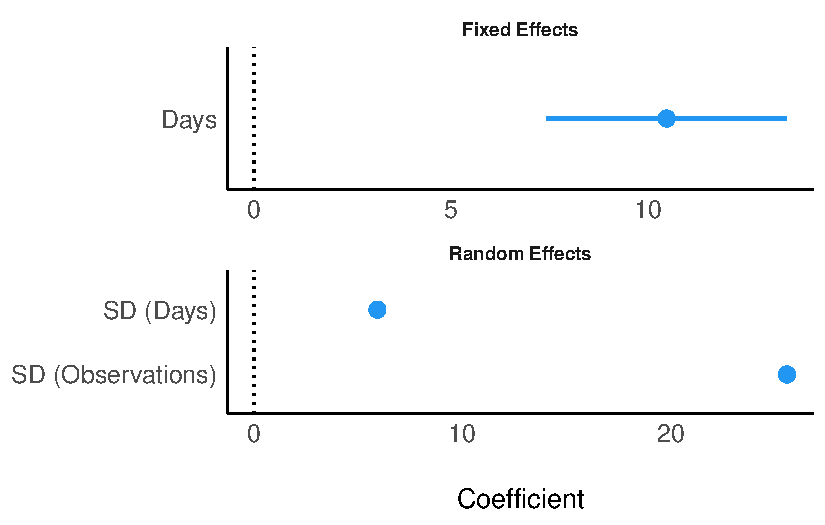
\includegraphics[keepaspectratio]{chapters/reporting_files/figure-pdf/unnamed-chunk-8-1.pdf}}

\begin{Shaded}
\begin{Highlighting}[]
\CommentTok{\# check assumptions of random effects}
\NormalTok{result }\OtherTok{\textless{}{-}} \FunctionTok{check\_normality}\NormalTok{(model, }\AttributeTok{effects =} \StringTok{"random"}\NormalTok{)}
\FunctionTok{plot}\NormalTok{(result)}
\end{Highlighting}
\end{Shaded}

\begin{verbatim}
[[1]]
\end{verbatim}

\pandocbounded{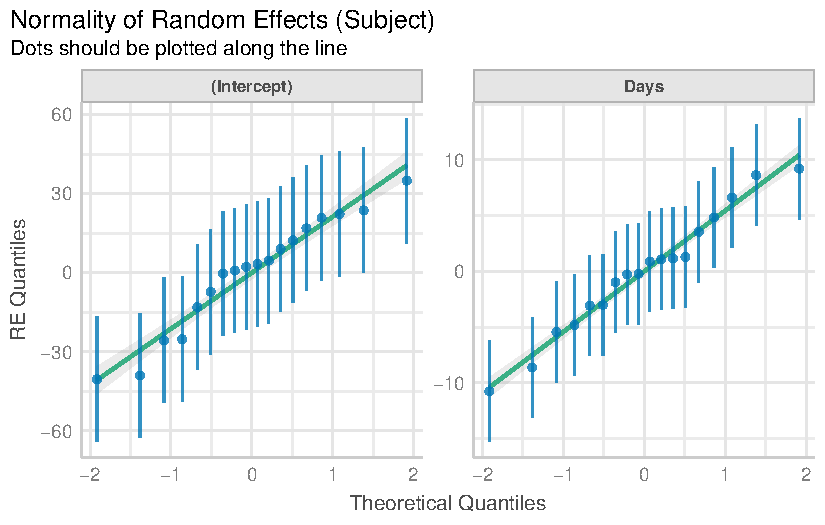
\includegraphics[keepaspectratio]{chapters/reporting_files/figure-pdf/unnamed-chunk-8-2.pdf}}

\subsection{ANOVAs}\label{anovas}

\begin{Shaded}
\begin{Highlighting}[]
\CommentTok{\# fit model}
\NormalTok{model }\OtherTok{\textless{}{-}} \FunctionTok{aov}\NormalTok{(mpg }\SpecialCharTok{\textasciitilde{}} \FunctionTok{factor}\NormalTok{(gear) }\SpecialCharTok{+} \FunctionTok{factor}\NormalTok{(carb), }\AttributeTok{data =}\NormalTok{ mtcars)}

\CommentTok{\# commonly used effect size: partial eta squared}
\FunctionTok{eta\_squared}\NormalTok{(model)}
\end{Highlighting}
\end{Shaded}

\begin{verbatim}
# Effect Size for ANOVA (Type I)

Parameter    | Eta2 (partial) |       95% CI
--------------------------------------------
factor(gear) |           0.69 | [0.49, 1.00]
factor(carb) |           0.66 | [0.41, 1.00]

- One-sided CIs: upper bound fixed at [1.00].
\end{verbatim}

\begin{Shaded}
\begin{Highlighting}[]
\CommentTok{\# better effect size: partialomega squared}
\FunctionTok{omega\_squared}\NormalTok{(model)}
\end{Highlighting}
\end{Shaded}

\begin{verbatim}
# Effect Size for ANOVA (Type I)

Parameter    | Omega2 (partial) |       95% CI
----------------------------------------------
factor(gear) |             0.62 | [0.38, 1.00]
factor(carb) |             0.57 | [0.26, 1.00]

- One-sided CIs: upper bound fixed at [1.00].
\end{verbatim}

\section{Summary statistics}\label{summary-statistics}

\begin{Shaded}
\begin{Highlighting}[]
\CommentTok{\# all columns}
\NormalTok{iris }\SpecialCharTok{|\textgreater{}}
  \FunctionTok{group\_by}\NormalTok{(Species) }\SpecialCharTok{|\textgreater{}}
  \FunctionTok{report\_table}\NormalTok{() }
\end{Highlighting}
\end{Shaded}

\begin{verbatim}
Group      |     Variable | n_Obs | Mean |   SD | Median |  MAD |  Min |  Max
-----------------------------------------------------------------------------
setosa     | Sepal.Length |    50 | 5.01 | 0.35 |   5.00 | 0.30 | 4.30 | 5.80
setosa     |  Sepal.Width |    50 | 3.43 | 0.38 |   3.40 | 0.37 | 2.30 | 4.40
setosa     | Petal.Length |    50 | 1.46 | 0.17 |   1.50 | 0.15 | 1.00 | 1.90
setosa     |  Petal.Width |    50 | 0.25 | 0.11 |   0.20 | 0.00 | 0.10 | 0.60
versicolor | Sepal.Length |    50 | 5.94 | 0.52 |   5.90 | 0.52 | 4.90 | 7.00
versicolor |  Sepal.Width |    50 | 2.77 | 0.31 |   2.80 | 0.30 | 2.00 | 3.40
versicolor | Petal.Length |    50 | 4.26 | 0.47 |   4.35 | 0.52 | 3.00 | 5.10
versicolor |  Petal.Width |    50 | 1.33 | 0.20 |   1.30 | 0.22 | 1.00 | 1.80
virginica  | Sepal.Length |    50 | 6.59 | 0.64 |   6.50 | 0.59 | 4.90 | 7.90
virginica  |  Sepal.Width |    50 | 2.97 | 0.32 |   3.00 | 0.30 | 2.20 | 3.80
virginica  | Petal.Length |    50 | 5.55 | 0.55 |   5.55 | 0.67 | 4.50 | 6.90
virginica  |  Petal.Width |    50 | 2.03 | 0.27 |   2.00 | 0.30 | 1.40 | 2.50

Group      | Skewness | Kurtosis | n_Missing
--------------------------------------------
setosa     |     0.12 |    -0.25 |         0
setosa     |     0.04 |     0.95 |         0
setosa     |     0.11 |     1.02 |         0
setosa     |     1.25 |     1.72 |         0
versicolor |     0.11 |    -0.53 |         0
versicolor |    -0.36 |    -0.37 |         0
versicolor |    -0.61 |     0.05 |         0
versicolor |    -0.03 |    -0.41 |         0
virginica  |     0.12 |     0.03 |         0
virginica  |     0.37 |     0.71 |         0
virginica  |     0.55 |    -0.15 |         0
virginica  |    -0.13 |    -0.60 |         0
\end{verbatim}

\begin{Shaded}
\begin{Highlighting}[]
\CommentTok{\# all columns {-} html output with rounding}
\NormalTok{iris }\SpecialCharTok{|\textgreater{}}
  \FunctionTok{group\_by}\NormalTok{(Species) }\SpecialCharTok{|\textgreater{}}
  \FunctionTok{report\_table}\NormalTok{() }\SpecialCharTok{|\textgreater{}}
  \FunctionTok{mutate\_if}\NormalTok{(is.numeric, round\_half\_up, }\AttributeTok{digits =} \DecValTok{2}\NormalTok{) }\SpecialCharTok{|\textgreater{}}
  \FunctionTok{kable}\NormalTok{() }\SpecialCharTok{|\textgreater{}}
  \FunctionTok{kable\_classic}\NormalTok{(}\AttributeTok{full\_width =} \ConstantTok{FALSE}\NormalTok{)}
\end{Highlighting}
\end{Shaded}

\begin{longtable*}[t]{llrrrrrrrrrr}
\toprule
Group & Variable & n\_Obs & Mean & SD & Median & MAD & Min & Max & Skewness & Kurtosis & n\_Missing\\
\midrule
setosa & Sepal.Length & 50 & 5.01 & 0.35 & 5.00 & 0.30 & 4.3 & 5.8 & 0.12 & -0.25 & 0\\
setosa & Sepal.Width & 50 & 3.43 & 0.38 & 3.40 & 0.37 & 2.3 & 4.4 & 0.04 & 0.95 & 0\\
setosa & Petal.Length & 50 & 1.46 & 0.17 & 1.50 & 0.15 & 1.0 & 1.9 & 0.11 & 1.02 & 0\\
setosa & Petal.Width & 50 & 0.25 & 0.11 & 0.20 & 0.00 & 0.1 & 0.6 & 1.25 & 1.72 & 0\\
versicolor & Sepal.Length & 50 & 5.94 & 0.52 & 5.90 & 0.52 & 4.9 & 7.0 & 0.11 & -0.53 & 0\\
\addlinespace
versicolor & Sepal.Width & 50 & 2.77 & 0.31 & 2.80 & 0.30 & 2.0 & 3.4 & -0.36 & -0.37 & 0\\
versicolor & Petal.Length & 50 & 4.26 & 0.47 & 4.35 & 0.52 & 3.0 & 5.1 & -0.61 & 0.05 & 0\\
versicolor & Petal.Width & 50 & 1.33 & 0.20 & 1.30 & 0.22 & 1.0 & 1.8 & -0.03 & -0.41 & 0\\
virginica & Sepal.Length & 50 & 6.59 & 0.64 & 6.50 & 0.59 & 4.9 & 7.9 & 0.12 & 0.03 & 0\\
virginica & Sepal.Width & 50 & 2.97 & 0.32 & 3.00 & 0.30 & 2.2 & 3.8 & 0.37 & 0.71 & 0\\
\addlinespace
virginica & Petal.Length & 50 & 5.55 & 0.55 & 5.55 & 0.67 & 4.5 & 6.9 & 0.55 & -0.15 & 0\\
virginica & Petal.Width & 50 & 2.03 & 0.27 & 2.00 & 0.30 & 1.4 & 2.5 & -0.13 & -0.60 & 0\\
\bottomrule
\end{longtable*}

\begin{Shaded}
\begin{Highlighting}[]
\CommentTok{\# subset of columns}
\NormalTok{iris }\SpecialCharTok{|\textgreater{}}
  \FunctionTok{group\_by}\NormalTok{(Species) }\SpecialCharTok{|\textgreater{}}
  \FunctionTok{report\_table}\NormalTok{() }\SpecialCharTok{|\textgreater{}}
  \FunctionTok{select}\NormalTok{(Group, Variable, n\_Obs, Mean, SD) }\SpecialCharTok{|\textgreater{}}
  \FunctionTok{mutate\_if}\NormalTok{(is.numeric, round\_half\_up, }\AttributeTok{digits =} \DecValTok{2}\NormalTok{) }\SpecialCharTok{|\textgreater{}}
  \FunctionTok{kable}\NormalTok{() }\SpecialCharTok{|\textgreater{}}
  \FunctionTok{kable\_classic}\NormalTok{(}\AttributeTok{full\_width =} \ConstantTok{FALSE}\NormalTok{)}
\end{Highlighting}
\end{Shaded}

\begin{longtable*}[t]{llrrr}
\toprule
Group & Variable & n\_Obs & Mean & SD\\
\midrule
setosa & Sepal.Length & 50 & 5.01 & 0.35\\
setosa & Sepal.Width & 50 & 3.43 & 0.38\\
setosa & Petal.Length & 50 & 1.46 & 0.17\\
setosa & Petal.Width & 50 & 0.25 & 0.11\\
versicolor & Sepal.Length & 50 & 5.94 & 0.52\\
\addlinespace
versicolor & Sepal.Width & 50 & 2.77 & 0.31\\
versicolor & Petal.Length & 50 & 4.26 & 0.47\\
versicolor & Petal.Width & 50 & 1.33 & 0.20\\
virginica & Sepal.Length & 50 & 6.59 & 0.64\\
virginica & Sepal.Width & 50 & 2.97 & 0.32\\
\addlinespace
virginica & Petal.Length & 50 & 5.55 & 0.55\\
virginica & Petal.Width & 50 & 2.03 & 0.27\\
\bottomrule
\end{longtable*}

\section{Assumption checks}\label{assumption-checks}

Beware that checking assumptions can lead to as many bad practices as it
does good ones! (e.g., poorly justified post hoc outlier exclusion)

\subsection{Multiple checks at once}\label{multiple-checks-at-once}

\begin{Shaded}
\begin{Highlighting}[]
\CommentTok{\# fit model}
\NormalTok{model }\OtherTok{\textless{}{-}} \FunctionTok{lm}\NormalTok{(wt }\SpecialCharTok{\textasciitilde{}} \DecValTok{1} \SpecialCharTok{+}\NormalTok{ am }\SpecialCharTok{+}\NormalTok{ mpg, }\AttributeTok{data =}\NormalTok{ mtcars)}

\CommentTok{\# check multiple model assumptions}
\FunctionTok{check\_model}\NormalTok{(model)}
\end{Highlighting}
\end{Shaded}

\pandocbounded{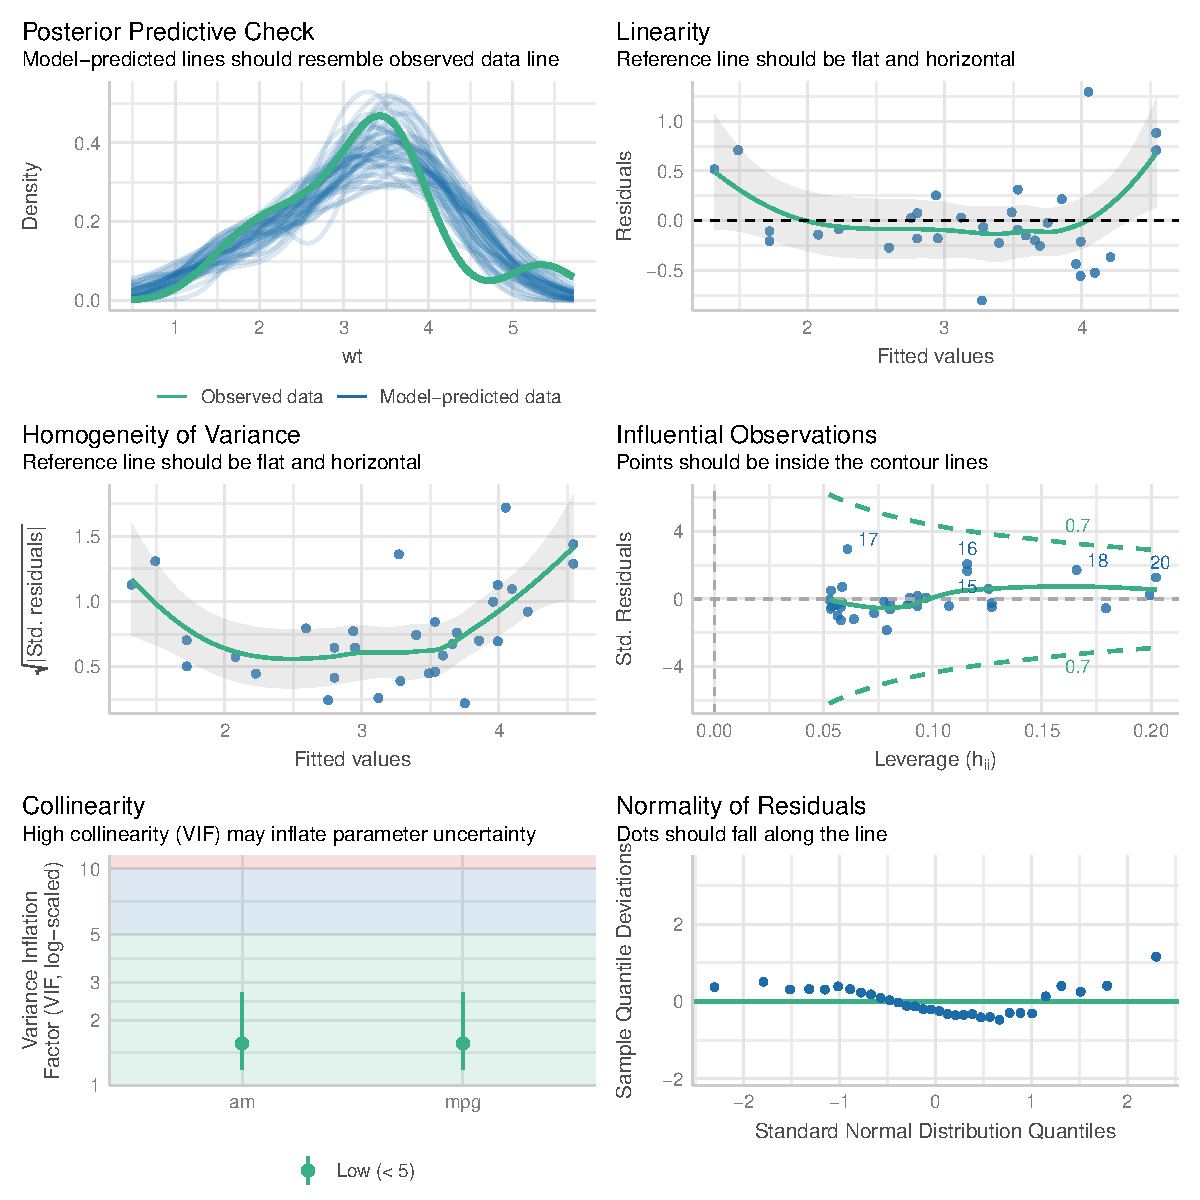
\includegraphics[keepaspectratio]{chapters/reporting_files/figure-pdf/unnamed-chunk-11-1.pdf}}

\subsection{Normality of distribution of
residuals}\label{normality-of-distribution-of-residuals}

\begin{Shaded}
\begin{Highlighting}[]
\NormalTok{res\_normality }\OtherTok{\textless{}{-}} \FunctionTok{check\_normality}\NormalTok{(model)}

\NormalTok{res\_normality}
\end{Highlighting}
\end{Shaded}

\begin{verbatim}
Warning: Non-normality of residuals detected (p = 0.013).
\end{verbatim}

\begin{Shaded}
\begin{Highlighting}[]
\FunctionTok{plot}\NormalTok{(res\_normality, }\AttributeTok{type =} \StringTok{"qq"}\NormalTok{)}
\end{Highlighting}
\end{Shaded}

\begin{verbatim}
For confidence bands, please install `qqplotr`.
\end{verbatim}

\pandocbounded{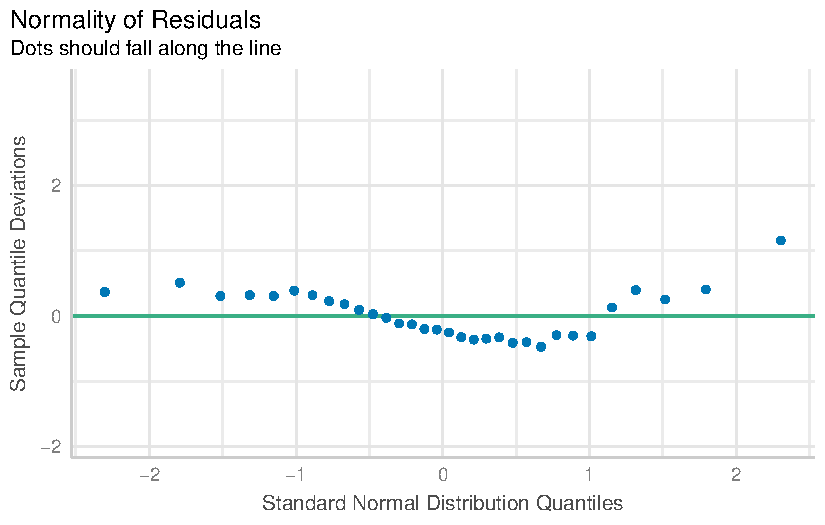
\includegraphics[keepaspectratio]{chapters/reporting_files/figure-pdf/unnamed-chunk-12-1.pdf}}

\begin{Shaded}
\begin{Highlighting}[]
\FunctionTok{plot}\NormalTok{(res\_normality, }\AttributeTok{type =} \StringTok{"density"}\NormalTok{)}
\end{Highlighting}
\end{Shaded}

\pandocbounded{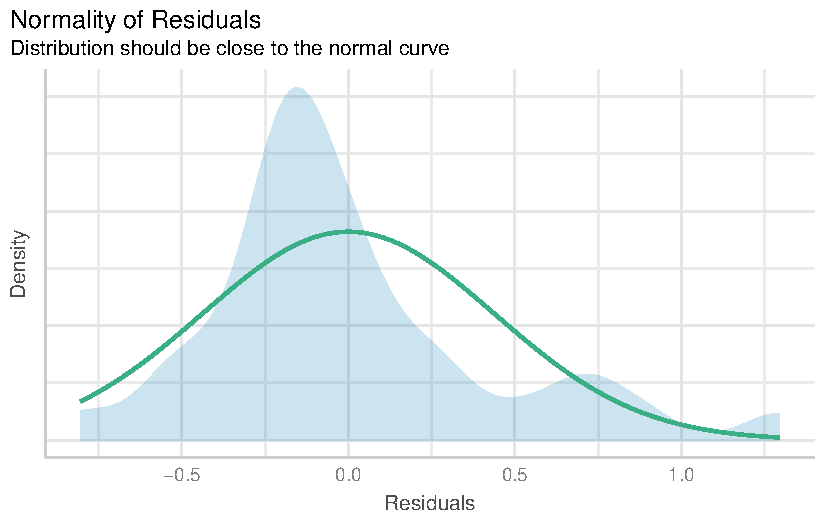
\includegraphics[keepaspectratio]{chapters/reporting_files/figure-pdf/unnamed-chunk-12-2.pdf}}

\subsection{Multicolinearity}\label{multicolinearity}

\begin{Shaded}
\begin{Highlighting}[]
\NormalTok{res\_collinearity }\OtherTok{\textless{}{-}} \FunctionTok{check\_collinearity}\NormalTok{(model)}

\NormalTok{res\_collinearity}
\end{Highlighting}
\end{Shaded}

\begin{verbatim}
# Check for Multicollinearity

Low Correlation

 Term  VIF   VIF 95% CI Increased SE Tolerance Tolerance 95% CI
   am 1.56 [1.19, 2.68]         1.25      0.64     [0.37, 0.84]
  mpg 1.56 [1.19, 2.68]         1.25      0.64     [0.37, 0.84]
\end{verbatim}

\begin{Shaded}
\begin{Highlighting}[]
\FunctionTok{plot}\NormalTok{(res\_collinearity)}
\end{Highlighting}
\end{Shaded}

\pandocbounded{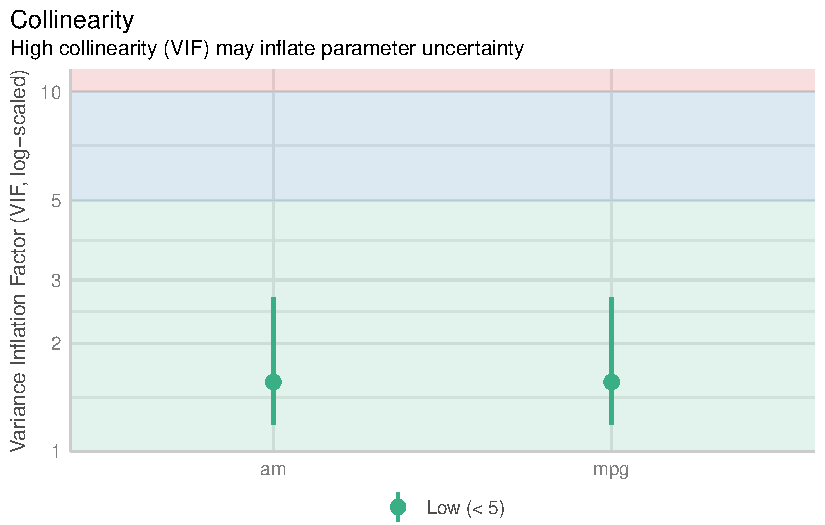
\includegraphics[keepaspectratio]{chapters/reporting_files/figure-pdf/unnamed-chunk-13-1.pdf}}

\subsection{Outliers}\label{outliers}

\begin{Shaded}
\begin{Highlighting}[]
\NormalTok{res\_outliers }\OtherTok{\textless{}{-}} \FunctionTok{check\_outliers}\NormalTok{(model, }\AttributeTok{method =} \StringTok{"cook"}\NormalTok{) }\CommentTok{\# "all" requires other dependencies and can take some time to run  }
\CommentTok{\#res\_outliers \textless{}{-} check\_outliers(model, method = "all") \# "all" requires other dependencies and can take some time to run  }

\NormalTok{res\_outliers}
\end{Highlighting}
\end{Shaded}

\begin{verbatim}
OK: No outliers detected.
- Based on the following method and threshold: cook (0.808).
- For variable: (Whole model)
\end{verbatim}

\begin{Shaded}
\begin{Highlighting}[]
\FunctionTok{plot}\NormalTok{(res\_outliers)}
\end{Highlighting}
\end{Shaded}

\pandocbounded{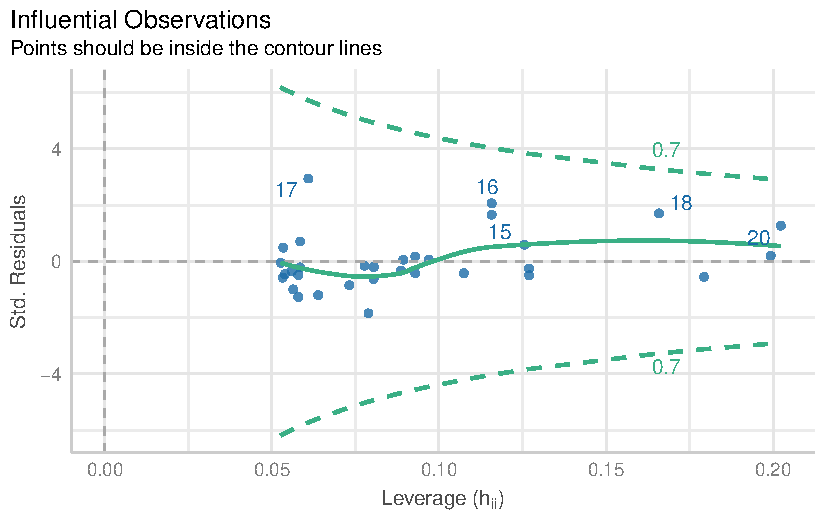
\includegraphics[keepaspectratio]{chapters/reporting_files/figure-pdf/unnamed-chunk-14-1.pdf}}

\subsection{Heteroscedasticity}\label{heteroscedasticity}

\begin{Shaded}
\begin{Highlighting}[]
\NormalTok{res\_het }\OtherTok{\textless{}{-}} \FunctionTok{check\_heteroscedasticity}\NormalTok{(model)}

\NormalTok{res\_het}
\end{Highlighting}
\end{Shaded}

\begin{verbatim}
OK: Error variance appears to be homoscedastic (p = 0.053).
\end{verbatim}

\begin{Shaded}
\begin{Highlighting}[]
\FunctionTok{plot}\NormalTok{(res\_het)}
\end{Highlighting}
\end{Shaded}

\pandocbounded{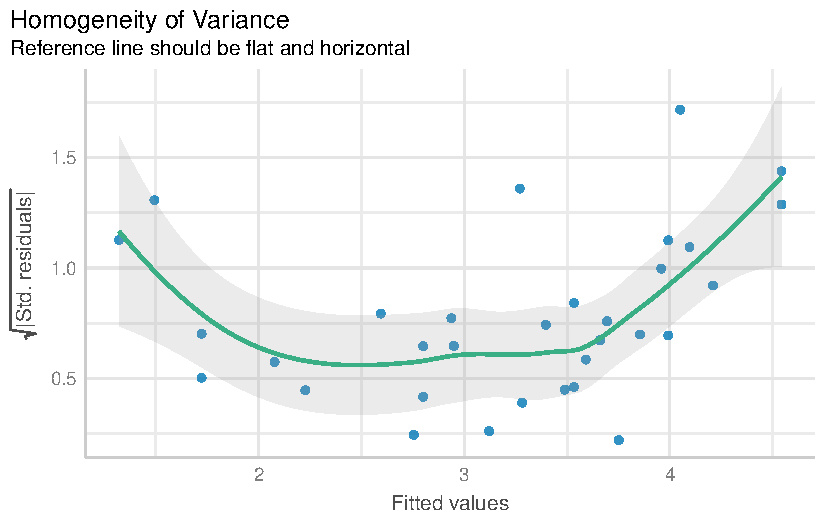
\includegraphics[keepaspectratio]{chapters/reporting_files/figure-pdf/unnamed-chunk-15-1.pdf}}

\bookmarksetup{startatroot}

\chapter{Visualization}\label{visualization}

\bookmarksetup{startatroot}

\chapter{Dependencies}\label{dependencies-5}

\begin{Shaded}
\begin{Highlighting}[]
\FunctionTok{library}\NormalTok{(readr)}
\FunctionTok{library}\NormalTok{(ggplot2)}
\CommentTok{\# install.packages("datasauRus")}
\FunctionTok{library}\NormalTok{(datasauRus) }
\FunctionTok{library}\NormalTok{(scales)}
\FunctionTok{library}\NormalTok{(dplyr)}
\FunctionTok{library}\NormalTok{(tidyr)}
\FunctionTok{library}\NormalTok{(plotrix) }

\CommentTok{\# install.packages("devtools")}
\CommentTok{\# devtools::install\_github("matthewbjane/ThemePark")}
\FunctionTok{library}\NormalTok{(ThemePark)}
\FunctionTok{library}\NormalTok{(patchwork)}
\FunctionTok{library}\NormalTok{(janitor)}
\FunctionTok{library}\NormalTok{(knitr)}
\FunctionTok{library}\NormalTok{(kableExtra)}
\end{Highlighting}
\end{Shaded}

\bookmarksetup{startatroot}

\chapter{Why plot data?}\label{why-plot-data}

Summary statistics aren't enough!

\begin{Shaded}
\begin{Highlighting}[]
\CommentTok{\# M and SD}
\NormalTok{datasaurus\_dozen }\SpecialCharTok{|\textgreater{}}
  \FunctionTok{group\_by}\NormalTok{(dataset) }\SpecialCharTok{|\textgreater{}}
  \FunctionTok{summarize}\NormalTok{(}\AttributeTok{mean\_x =} \FunctionTok{mean}\NormalTok{(x),}
            \AttributeTok{sd\_x =} \FunctionTok{sd}\NormalTok{(x),}
            \AttributeTok{mean\_y =} \FunctionTok{mean}\NormalTok{(y),}
            \AttributeTok{sd\_y =} \FunctionTok{sd}\NormalTok{(y)) }\SpecialCharTok{|\textgreater{}}
  \FunctionTok{mutate\_if}\NormalTok{(is.numeric, round\_half\_up, }\AttributeTok{digits =} \DecValTok{2}\NormalTok{) }\SpecialCharTok{|\textgreater{}}
  \FunctionTok{kable}\NormalTok{(}\AttributeTok{align =} \StringTok{\textquotesingle{}r\textquotesingle{}}\NormalTok{)}\SpecialCharTok{|\textgreater{}}
  \FunctionTok{kable\_classic}\NormalTok{(}\AttributeTok{full\_width =} \ConstantTok{FALSE}\NormalTok{)}
\end{Highlighting}
\end{Shaded}

\begin{longtable*}[t]{rrrrr}
\toprule
dataset & mean\_x & sd\_x & mean\_y & sd\_y\\
\midrule
away & 54.27 & 16.77 & 47.83 & 26.94\\
bullseye & 54.27 & 16.77 & 47.83 & 26.94\\
circle & 54.27 & 16.76 & 47.84 & 26.93\\
dino & 54.26 & 16.77 & 47.83 & 26.94\\
dots & 54.26 & 16.77 & 47.84 & 26.93\\
\addlinespace
h\_lines & 54.26 & 16.77 & 47.83 & 26.94\\
high\_lines & 54.27 & 16.77 & 47.84 & 26.94\\
slant\_down & 54.27 & 16.77 & 47.84 & 26.94\\
slant\_up & 54.27 & 16.77 & 47.83 & 26.94\\
star & 54.27 & 16.77 & 47.84 & 26.93\\
\addlinespace
v\_lines & 54.27 & 16.77 & 47.84 & 26.94\\
wide\_lines & 54.27 & 16.77 & 47.83 & 26.94\\
x\_shape & 54.26 & 16.77 & 47.84 & 26.93\\
\bottomrule
\end{longtable*}

\begin{Shaded}
\begin{Highlighting}[]
\CommentTok{\# correlation}
\NormalTok{datasaurus\_dozen }\SpecialCharTok{|\textgreater{}}
  \FunctionTok{group\_by}\NormalTok{(dataset) }\SpecialCharTok{|\textgreater{}}
  \FunctionTok{summarize}\NormalTok{(}\AttributeTok{correlation =} \FunctionTok{cor}\NormalTok{(x, y)) }\SpecialCharTok{|\textgreater{}}
  \FunctionTok{mutate\_if}\NormalTok{(is.numeric, round\_half\_up, }\AttributeTok{digits =} \DecValTok{2}\NormalTok{) }\SpecialCharTok{|\textgreater{}}
  \FunctionTok{kable}\NormalTok{(}\AttributeTok{align =} \StringTok{\textquotesingle{}r\textquotesingle{}}\NormalTok{) }\SpecialCharTok{|\textgreater{}}
  \FunctionTok{kable\_classic}\NormalTok{(}\AttributeTok{full\_width =} \ConstantTok{FALSE}\NormalTok{)}
\end{Highlighting}
\end{Shaded}

\begin{longtable*}[t]{rr}
\toprule
dataset & correlation\\
\midrule
away & -0.06\\
bullseye & -0.07\\
circle & -0.07\\
dino & -0.06\\
dots & -0.06\\
\addlinespace
h\_lines & -0.06\\
high\_lines & -0.07\\
slant\_down & -0.07\\
slant\_up & -0.07\\
star & -0.06\\
\addlinespace
v\_lines & -0.07\\
wide\_lines & -0.07\\
x\_shape & -0.07\\
\bottomrule
\end{longtable*}

Always plot your data!

\begin{Shaded}
\begin{Highlighting}[]
\FunctionTok{ggplot}\NormalTok{(datasaurus\_dozen, }\FunctionTok{aes}\NormalTok{(}\AttributeTok{x =}\NormalTok{ x, }\AttributeTok{y =}\NormalTok{ y)) }\SpecialCharTok{+}
  \FunctionTok{geom\_point}\NormalTok{() }\SpecialCharTok{+}
  \FunctionTok{facet\_wrap}\NormalTok{(}\SpecialCharTok{\textasciitilde{}}\NormalTok{dataset) }\SpecialCharTok{+}
  \FunctionTok{theme\_minimal}\NormalTok{()}
\end{Highlighting}
\end{Shaded}

\pandocbounded{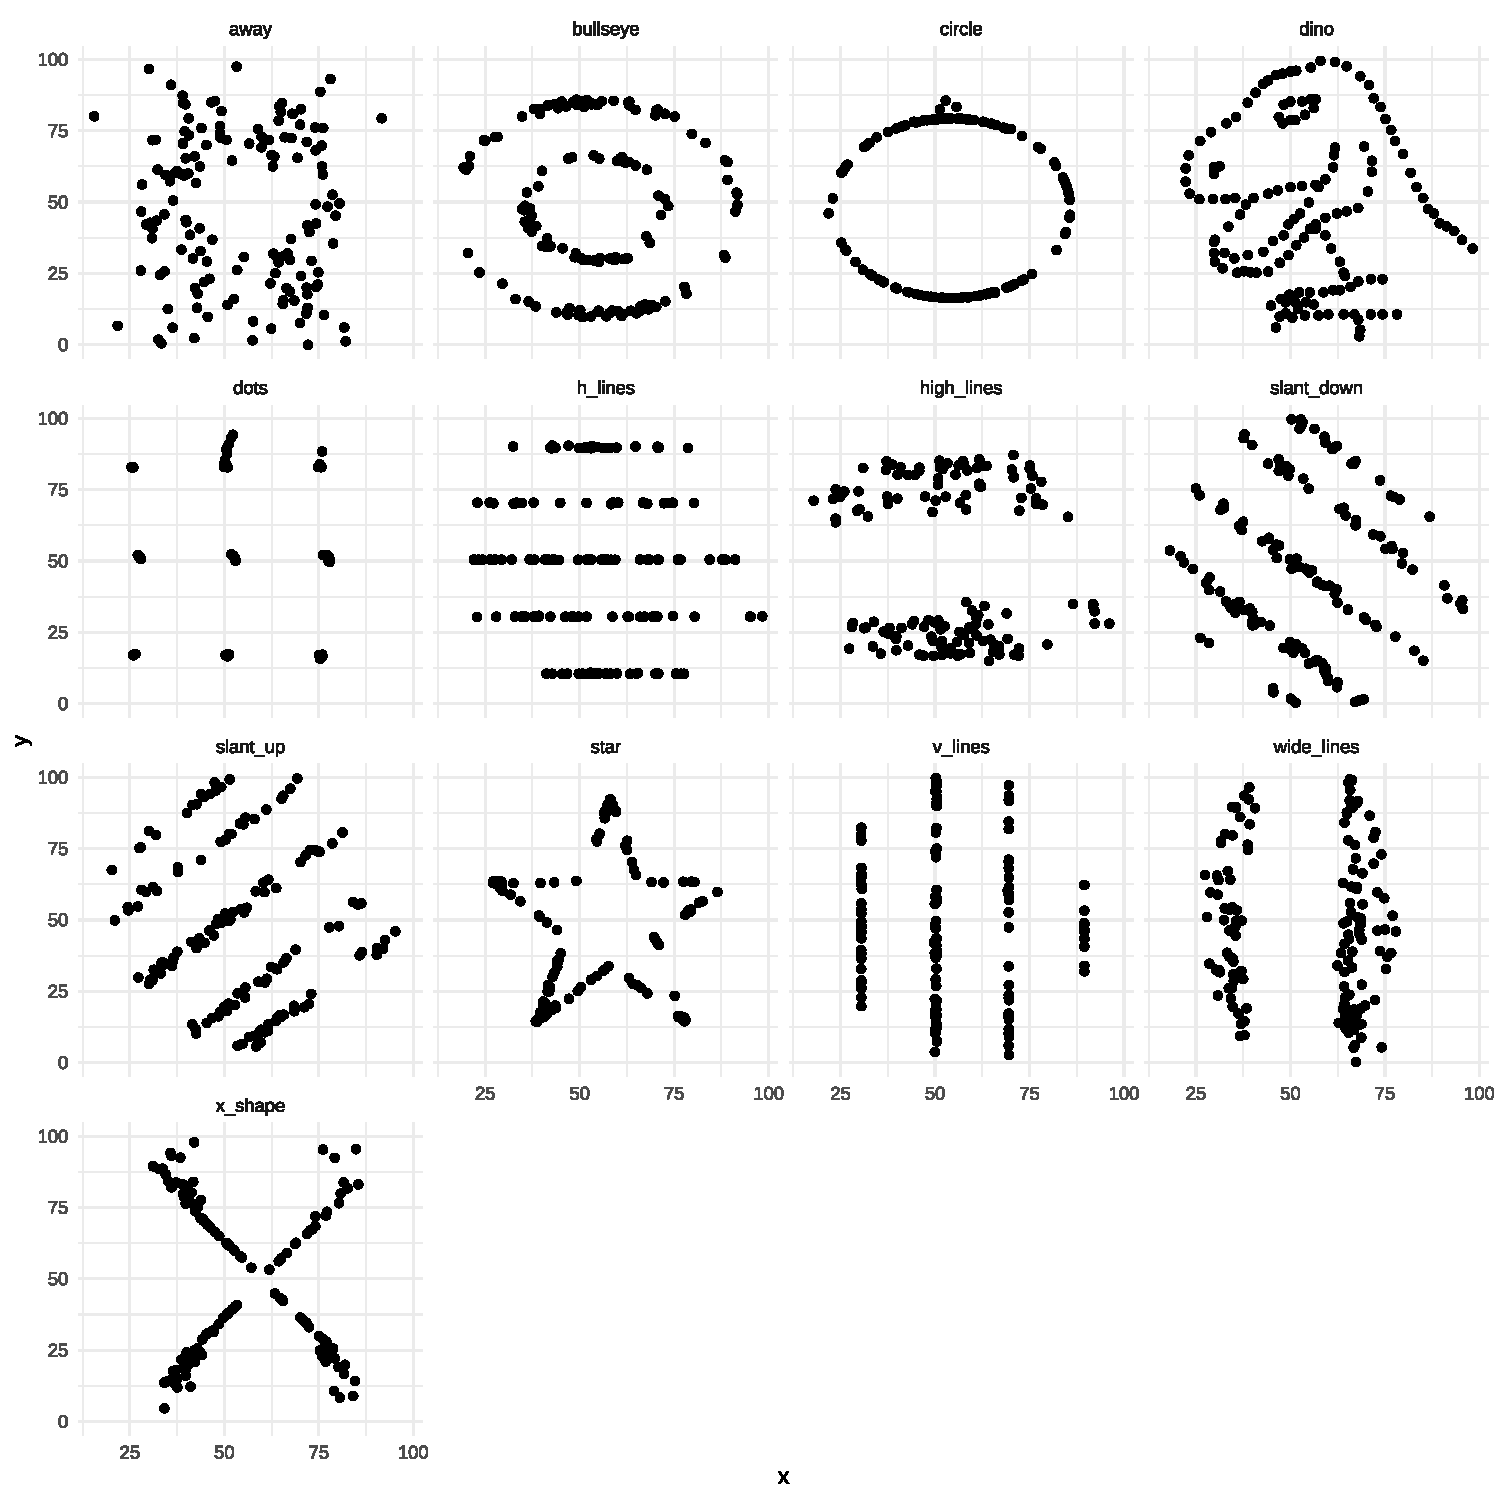
\includegraphics[keepaspectratio]{chapters/visualization_files/figure-pdf/unnamed-chunk-4-1.pdf}}

\bookmarksetup{startatroot}

\chapter{Structure of a ggplot}\label{structure-of-a-ggplot}

Whereas the pipes (\texttt{\%\textgreater{}\%} and
\texttt{\textbar{}\textgreater{}}) are used to create tidy data
wrangling and analysis workflows, ggplot functions are added together
with \texttt{+}.

Function calls are applied in order as layers. Changing the order
functions are called can therefore change the appearance of the plot.

\begin{Shaded}
\begin{Highlighting}[]
\CommentTok{\# get data}
\NormalTok{data\_processed }\OtherTok{\textless{}{-}} \FunctionTok{read\_csv}\NormalTok{(}\StringTok{"../data/processed/data\_processed.csv"}\NormalTok{)}

\NormalTok{data\_after\_exclusions }\OtherTok{\textless{}{-}}\NormalTok{ data\_processed }\SpecialCharTok{|\textgreater{}}
  \FunctionTok{filter}\NormalTok{(exclude\_amp }\SpecialCharTok{==} \StringTok{"include"} \SpecialCharTok{\&} 
\NormalTok{           n\_items }\SpecialCharTok{==} \DecValTok{3} \SpecialCharTok{\&} 
\NormalTok{           gender }\SpecialCharTok{\%in\%} \FunctionTok{c}\NormalTok{(}\StringTok{"male"}\NormalTok{, }\StringTok{"female"}\NormalTok{)) }
\end{Highlighting}
\end{Shaded}

\begin{Shaded}
\begin{Highlighting}[]
\CommentTok{\# data and aesthetics calls}
\NormalTok{plot\_1 }\OtherTok{\textless{}{-}} 
  \FunctionTok{ggplot}\NormalTok{(}\AttributeTok{data =}\NormalTok{ data\_after\_exclusions,}
         \FunctionTok{aes}\NormalTok{(}\AttributeTok{x =}\NormalTok{ mean\_self\_report,}
             \AttributeTok{y =}\NormalTok{ amp\_score,}
             \AttributeTok{color =}\NormalTok{ gender,}
             \AttributeTok{shape =}\NormalTok{ gender)) }\SpecialCharTok{+}
  \CommentTok{\# draw lines manually}
  \FunctionTok{geom\_vline}\NormalTok{(}\AttributeTok{xintercept =} \DecValTok{4}\NormalTok{, }\AttributeTok{linetype =} \StringTok{"dotted"}\NormalTok{) }\SpecialCharTok{+}
  \FunctionTok{geom\_hline}\NormalTok{(}\AttributeTok{yintercept =} \FloatTok{0.5}\NormalTok{, }\AttributeTok{linetype =} \StringTok{"dotted"}\NormalTok{) }\SpecialCharTok{+}
  \CommentTok{\# draw geoms using the aesthetics (x, y, color and shape)}
  \DocumentationTok{\#\# points}
  \FunctionTok{geom\_point}\NormalTok{() }\SpecialCharTok{+}
  \DocumentationTok{\#\# fit curves, in this case a linear model}
  \FunctionTok{geom\_smooth}\NormalTok{(}\AttributeTok{method =} \StringTok{"lm"}\NormalTok{) }\SpecialCharTok{+}
  \CommentTok{\# adjust axis labels and ranges}
  \FunctionTok{scale\_x\_continuous}\NormalTok{(}\AttributeTok{name =} \StringTok{"Explicit evaluation}\SpecialCharTok{\textbackslash{}n}\StringTok{(Self{-}report)"}\NormalTok{,}
                     \AttributeTok{breaks =}\NormalTok{ scales}\SpecialCharTok{::}\FunctionTok{breaks\_pretty}\NormalTok{(}\AttributeTok{n =} \DecValTok{7}\NormalTok{)) }\SpecialCharTok{+}
  \FunctionTok{scale\_y\_continuous}\NormalTok{(}\AttributeTok{name =} \StringTok{"Implicit evaluation}\SpecialCharTok{\textbackslash{}n}\StringTok{(AMP)"}\NormalTok{) }\SpecialCharTok{+}
  \CommentTok{\# apply a theme}
  \FunctionTok{theme\_linedraw}\NormalTok{() }\SpecialCharTok{+} 
  \CommentTok{\# adjust elements of the theme}
  \FunctionTok{labs}\NormalTok{(}\AttributeTok{title =} \StringTok{"Scatter plot with linear regression lines"}\NormalTok{,}
       \AttributeTok{color =} \StringTok{"Gender"}\NormalTok{,}
       \AttributeTok{shape =} \StringTok{"Gender"}\NormalTok{) }\SpecialCharTok{+}
  \CommentTok{\# adjust the colors }
  \FunctionTok{scale\_color\_manual}\NormalTok{(}\AttributeTok{values =} \FunctionTok{c}\NormalTok{(}\StringTok{"female"} \OtherTok{=} \StringTok{"\#FF69B4"}\NormalTok{,}
                                \StringTok{"male"} \OtherTok{=} \StringTok{"\#6495ED"}\NormalTok{),}
                     \AttributeTok{labels =} \FunctionTok{c}\NormalTok{(}\StringTok{"female"} \OtherTok{=} \StringTok{"Female"}\NormalTok{,}
                                \StringTok{"male"} \OtherTok{=} \StringTok{"Male"}\NormalTok{)) }\SpecialCharTok{+}
  \CommentTok{\# adjust the shapes}
  \FunctionTok{scale\_shape\_manual}\NormalTok{(}\AttributeTok{values =} \FunctionTok{c}\NormalTok{(}\StringTok{"female"} \OtherTok{=} \DecValTok{16}\NormalTok{, }
                                \StringTok{"male"} \OtherTok{=} \DecValTok{17}\NormalTok{),}
                     \AttributeTok{labels =} \FunctionTok{c}\NormalTok{(}\StringTok{"female"} \OtherTok{=} \StringTok{"Female"}\NormalTok{,}
                                \StringTok{"male"} \OtherTok{=} \StringTok{"Male"}\NormalTok{)) }\SpecialCharTok{+}
  \CommentTok{\# display specific x and y coordinates without dropping data points (nb using \textasciigrave{}limits\textasciigrave{} drops data points, coord\_cartesian does not) }
  \FunctionTok{coord\_cartesian}\NormalTok{(}\AttributeTok{xlim =} \FunctionTok{c}\NormalTok{(}\DecValTok{1}\NormalTok{, }\DecValTok{7}\NormalTok{),}
                  \AttributeTok{ylim =} \FunctionTok{c}\NormalTok{(}\DecValTok{0}\NormalTok{, }\DecValTok{1}\NormalTok{))}

\CommentTok{\# display plot below chunk}
\NormalTok{plot\_1}
\end{Highlighting}
\end{Shaded}

\pandocbounded{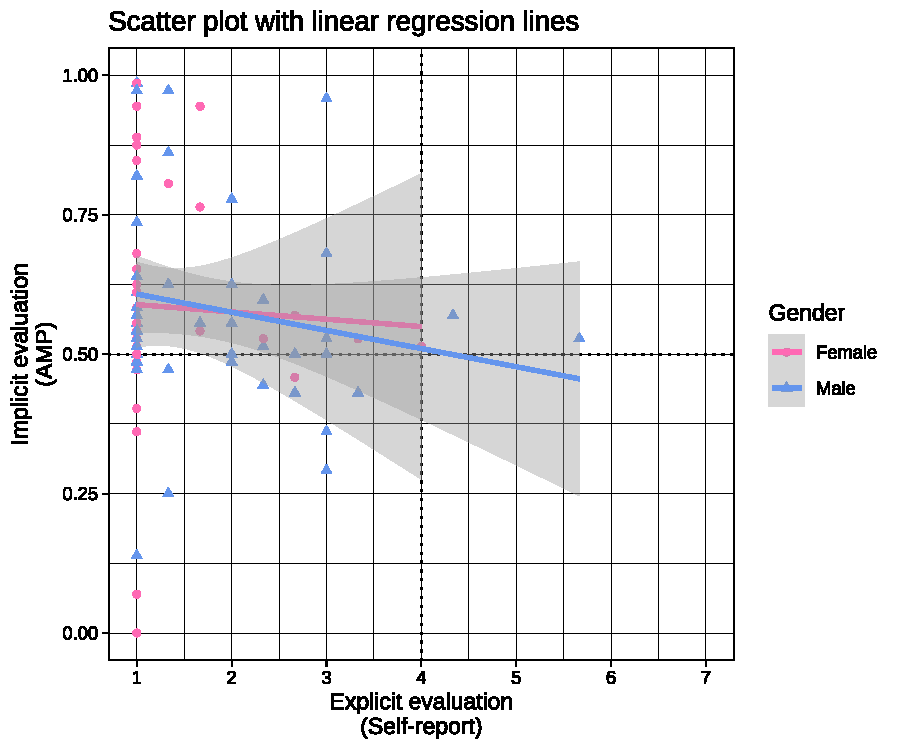
\includegraphics[keepaspectratio]{chapters/visualization_files/figure-pdf/unnamed-chunk-6-1.pdf}}

\begin{Shaded}
\begin{Highlighting}[]
\CommentTok{\# save plot to disk as pdf}
\FunctionTok{ggsave}\NormalTok{(}\AttributeTok{plot =}\NormalTok{ plot\_1,}
       \AttributeTok{filename =} \StringTok{"plots/plot\_1.pdf"}\NormalTok{, }
       \AttributeTok{width =} \DecValTok{6}\NormalTok{,}
       \AttributeTok{height =} \DecValTok{5}\NormalTok{)}
\end{Highlighting}
\end{Shaded}

Note that you can add additional function calls to objects later, e.g.,
overriding the previous theme\_ call with a new one:

\begin{Shaded}
\begin{Highlighting}[]
\NormalTok{plot\_1 }\SpecialCharTok{+} \FunctionTok{theme\_barbie}\NormalTok{()}
\end{Highlighting}
\end{Shaded}

\pandocbounded{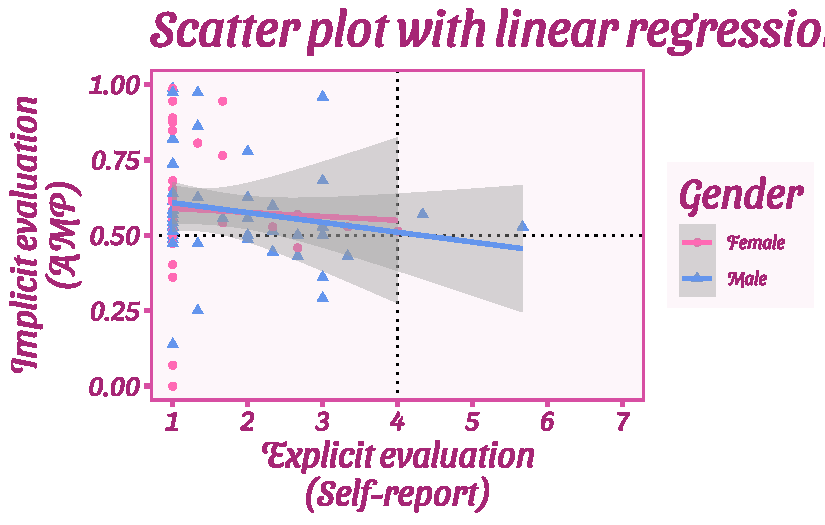
\includegraphics[keepaspectratio]{chapters/visualization_files/figure-pdf/unnamed-chunk-7-1.pdf}}

\bookmarksetup{startatroot}

\chapter{\texorpdfstring{Histogram using
\texttt{geom\_histogram()}}{Histogram using geom\_histogram()}}\label{histogram-using-geom_histogram}

\section{Simple plot for
self-reports}\label{simple-plot-for-self-reports}

\begin{Shaded}
\begin{Highlighting}[]
\FunctionTok{ggplot}\NormalTok{(}\AttributeTok{data =}\NormalTok{ data\_after\_exclusions,}
       \FunctionTok{aes}\NormalTok{(}\AttributeTok{x =}\NormalTok{ mean\_self\_report)) }\SpecialCharTok{+}
  \FunctionTok{geom\_histogram}\NormalTok{(}\AttributeTok{binwidth =} \DecValTok{1}\NormalTok{)}
\end{Highlighting}
\end{Shaded}

\pandocbounded{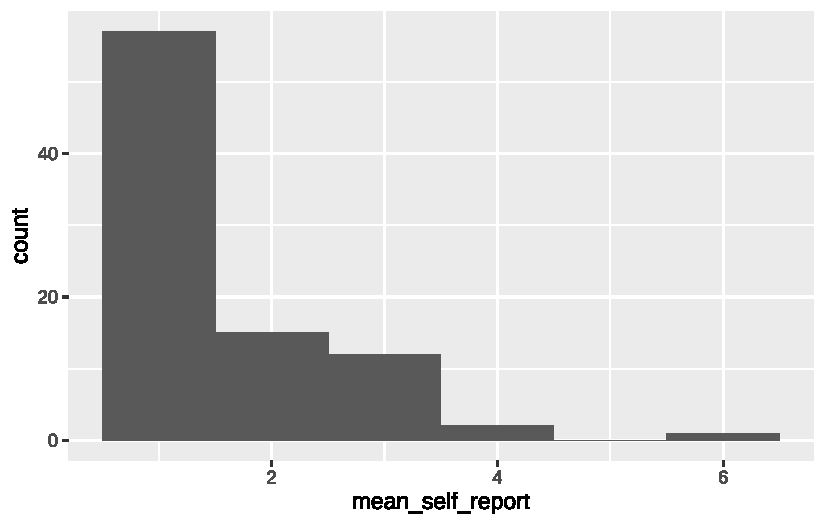
\includegraphics[keepaspectratio]{chapters/visualization_files/figure-pdf/unnamed-chunk-8-1.pdf}}

\section{Slightly better plot for
self-reports}\label{slightly-better-plot-for-self-reports}

\begin{Shaded}
\begin{Highlighting}[]
\FunctionTok{ggplot}\NormalTok{(}\AttributeTok{data =}\NormalTok{ data\_after\_exclusions,}
       \FunctionTok{aes}\NormalTok{(}\AttributeTok{x =}\NormalTok{ mean\_self\_report)) }\SpecialCharTok{+}
  \CommentTok{\# more intelligent choices for the binwidth and boundary}
  \FunctionTok{geom\_histogram}\NormalTok{(}\AttributeTok{binwidth =} \DecValTok{1}\NormalTok{, }\AttributeTok{boundary =} \FloatTok{0.5}\NormalTok{) }\SpecialCharTok{+}
  \CommentTok{\# labeling of the axis points}
  \FunctionTok{scale\_x\_continuous}\NormalTok{(}\AttributeTok{breaks =}\NormalTok{ scales}\SpecialCharTok{::}\FunctionTok{breaks\_pretty}\NormalTok{(}\AttributeTok{n =} \DecValTok{7}\NormalTok{),}
                     \AttributeTok{limits =} \FunctionTok{c}\NormalTok{(}\FloatTok{0.5}\NormalTok{, }\FloatTok{7.5}\NormalTok{)) }\SpecialCharTok{+}
  \FunctionTok{scale\_y\_continuous}\NormalTok{(}\AttributeTok{breaks =} \FunctionTok{seq}\NormalTok{(}\DecValTok{0}\NormalTok{, }\DecValTok{60}\NormalTok{, }\DecValTok{10}\NormalTok{)) }\SpecialCharTok{+}
  \FunctionTok{theme\_minimal}\NormalTok{()}
\end{Highlighting}
\end{Shaded}

\pandocbounded{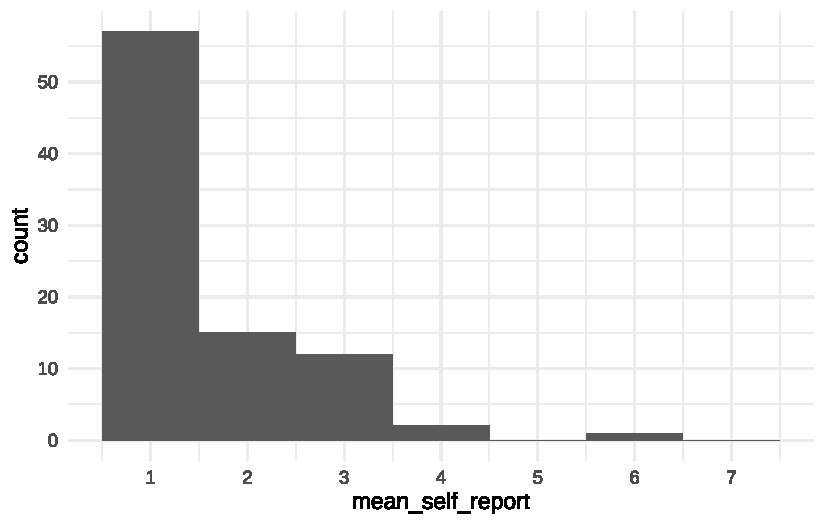
\includegraphics[keepaspectratio]{chapters/visualization_files/figure-pdf/unnamed-chunk-9-1.pdf}}

\section{Exercise: Plot for gender}\label{exercise-plot-for-gender}

Create a similar plot for the gender variable in
\texttt{data\_processed} (ie before exclusions).

\section{Exercise: Plot for AMP}\label{exercise-plot-for-amp}

Create a similar plot for the AMP scores in
\texttt{data\_after\_exclusions}.

\begin{Shaded}
\begin{Highlighting}[]
\NormalTok{mean\_amp }\OtherTok{\textless{}{-}}\NormalTok{ data\_after\_exclusions }\SpecialCharTok{|\textgreater{}}
  \FunctionTok{summarize}\NormalTok{(}\AttributeTok{mean\_amp =} \FunctionTok{mean}\NormalTok{(amp\_score)) }\SpecialCharTok{|\textgreater{}}
  \FunctionTok{pull}\NormalTok{(mean\_amp)}


\NormalTok{plot\_amp }\OtherTok{\textless{}{-}} 
  \FunctionTok{ggplot}\NormalTok{(}\AttributeTok{data =}\NormalTok{ data\_after\_exclusions,}
         \FunctionTok{aes}\NormalTok{(}\AttributeTok{x =}\NormalTok{ amp\_score)) }\SpecialCharTok{+}
  \FunctionTok{geom\_histogram}\NormalTok{(}\AttributeTok{binwidth =} \FloatTok{0.1}\NormalTok{) }\SpecialCharTok{+}
  \FunctionTok{scale\_x\_continuous}\NormalTok{(}\AttributeTok{breaks =} \FunctionTok{seq}\NormalTok{(}\DecValTok{0}\NormalTok{, }\DecValTok{1}\NormalTok{, .}\DecValTok{10}\NormalTok{),}
                     \AttributeTok{name =} \StringTok{"AMP score"}\NormalTok{) }\SpecialCharTok{+}
  \FunctionTok{scale\_y\_continuous}\NormalTok{(}\AttributeTok{breaks =} \FunctionTok{seq}\NormalTok{(}\DecValTok{0}\NormalTok{, }\DecValTok{40}\NormalTok{, }\DecValTok{5}\NormalTok{),}
                     \AttributeTok{name =} \StringTok{"Frequency"}\NormalTok{) }\SpecialCharTok{+}
  \FunctionTok{geom\_vline}\NormalTok{(}\AttributeTok{xintercept =}\NormalTok{ mean\_amp, }\AttributeTok{linetype =} \StringTok{"dotted"}\NormalTok{) }\SpecialCharTok{+}
  \FunctionTok{theme\_linedraw}\NormalTok{()}

\NormalTok{plot\_amp}
\end{Highlighting}
\end{Shaded}

\pandocbounded{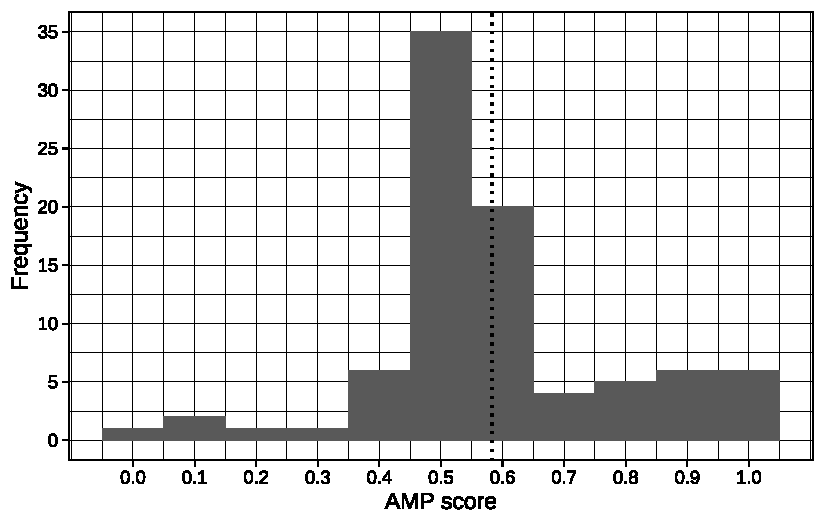
\includegraphics[keepaspectratio]{chapters/visualization_files/figure-pdf/unnamed-chunk-11-1.pdf}}

\begin{Shaded}
\begin{Highlighting}[]
\FunctionTok{ggsave}\NormalTok{(}\AttributeTok{plot =}\NormalTok{ plot\_amp,}
       \AttributeTok{filename =} \StringTok{"plots/plot\_amp.pdf"}\NormalTok{, }
       \AttributeTok{width =} \DecValTok{6}\NormalTok{,}
       \AttributeTok{height =} \DecValTok{5}\NormalTok{)}
\end{Highlighting}
\end{Shaded}

\begin{itemize}
\tightlist
\item
  Exercise: How to add a dashed vertical line at the sample's mean AMP
  score?
\end{itemize}

\bookmarksetup{startatroot}

\chapter{\texorpdfstring{Density plot using
\texttt{geom\_density()}}{Density plot using geom\_density()}}\label{density-plot-using-geom_density}

\section{Simple plot for
self-reports}\label{simple-plot-for-self-reports-1}

\begin{Shaded}
\begin{Highlighting}[]
\FunctionTok{ggplot}\NormalTok{(}\AttributeTok{data =}\NormalTok{ data\_after\_exclusions,}
       \FunctionTok{aes}\NormalTok{(}\AttributeTok{x =}\NormalTok{ mean\_self\_report)) }\SpecialCharTok{+}
  \FunctionTok{geom\_density}\NormalTok{(}\AttributeTok{adjust =} \DecValTok{1}\NormalTok{, }\CommentTok{\# the degree of smoothing can be adjusted here }
               \AttributeTok{color =} \StringTok{"\#FF69B4"}\NormalTok{,}
               \AttributeTok{fill =} \StringTok{"darkblue"}\NormalTok{, }
               \AttributeTok{alpha =} \FloatTok{0.3}\NormalTok{) }\SpecialCharTok{+}
  \CommentTok{\# labeling of the axis points}
  \FunctionTok{scale\_x\_continuous}\NormalTok{(}\AttributeTok{breaks =}\NormalTok{ scales}\SpecialCharTok{::}\FunctionTok{breaks\_pretty}\NormalTok{(}\AttributeTok{n =} \DecValTok{7}\NormalTok{),}
                     \AttributeTok{limits =} \FunctionTok{c}\NormalTok{(}\DecValTok{1}\NormalTok{, }\DecValTok{7}\NormalTok{)) }\SpecialCharTok{+}
  \FunctionTok{theme\_minimal}\NormalTok{()}
\end{Highlighting}
\end{Shaded}

\pandocbounded{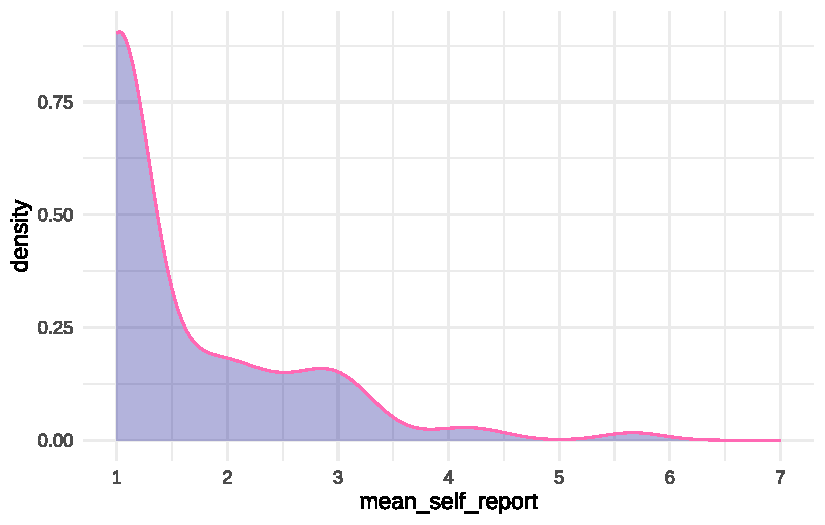
\includegraphics[keepaspectratio]{chapters/visualization_files/figure-pdf/unnamed-chunk-12-1.pdf}}

\section{Exercise: Plot for AMP}\label{exercise-plot-for-amp-1}

Make a similar density plot for the AMP.

\begin{itemize}
\tightlist
\item
  Add a theme.
\item
  Make the X axis breaks prettier.
\item
  Name both axis names more clearly.
\end{itemize}

\bookmarksetup{startatroot}

\chapter{\texorpdfstring{Bar plot using
\texttt{geom\_col()}}{Bar plot using geom\_col()}}\label{bar-plot-using-geom_col}

Bar plots are bad and usually shouldn't be used. But they are sometimes
unavoidable, so here's how to make them.

\section{Simple plot for AMP}\label{simple-plot-for-amp}

\begin{Shaded}
\begin{Highlighting}[]
\CommentTok{\# create the summary values to be plotted}
\NormalTok{summary\_amp }\OtherTok{\textless{}{-}}\NormalTok{ data\_after\_exclusions }\SpecialCharTok{\%\textgreater{}\%}
  \FunctionTok{group\_by}\NormalTok{(gender) }\SpecialCharTok{\%\textgreater{}\%}
  \FunctionTok{summarize}\NormalTok{(}\AttributeTok{amp\_mean =} \FunctionTok{mean}\NormalTok{(amp\_score),}
            \AttributeTok{amp\_se =}\NormalTok{ plotrix}\SpecialCharTok{::}\FunctionTok{std.error}\NormalTok{(amp\_score))}

\CommentTok{\# plot these values}
\FunctionTok{ggplot}\NormalTok{(}\AttributeTok{data =}\NormalTok{ summary\_amp, }
       \FunctionTok{aes}\NormalTok{(}\AttributeTok{x =}\NormalTok{ gender, }
           \AttributeTok{y =}\NormalTok{ amp\_mean)) }\SpecialCharTok{+}
  \FunctionTok{geom\_col}\NormalTok{() }\SpecialCharTok{+}
  \CommentTok{\# geom\_bar(stat = "identity") + \# NB geom\_col is equivalent to geom\_bar when stat == "identity}
  \FunctionTok{geom\_linerange}\NormalTok{(}\FunctionTok{aes}\NormalTok{(}\AttributeTok{ymin =}\NormalTok{ amp\_mean }\SpecialCharTok{{-}}\NormalTok{ amp\_se, }
                     \AttributeTok{ymax =}\NormalTok{ amp\_mean }\SpecialCharTok{+}\NormalTok{ amp\_se)) }
\end{Highlighting}
\end{Shaded}

\pandocbounded{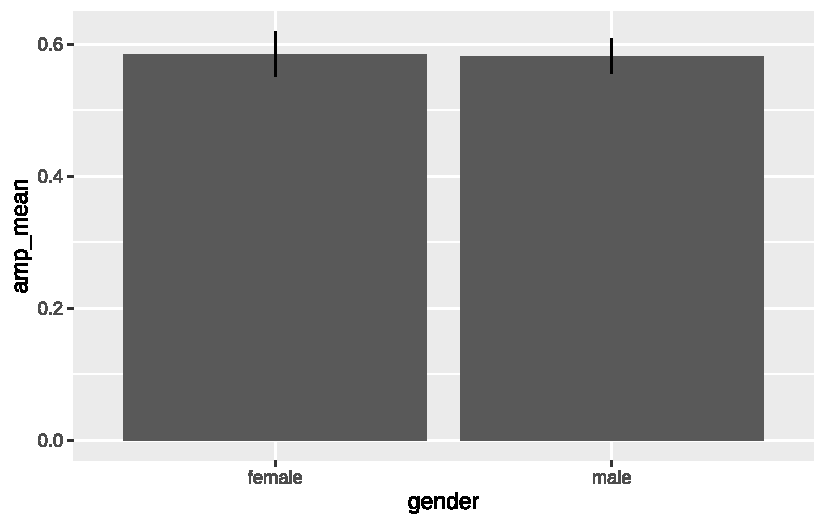
\includegraphics[keepaspectratio]{chapters/visualization_files/figure-pdf/unnamed-chunk-14-1.pdf}}

\section{Slightly better plot for
AMP}\label{slightly-better-plot-for-amp}

\begin{Shaded}
\begin{Highlighting}[]
\FunctionTok{ggplot}\NormalTok{(}\AttributeTok{data =}\NormalTok{ summary\_amp, }
       \FunctionTok{aes}\NormalTok{(}\AttributeTok{x =}\NormalTok{ gender, }
           \AttributeTok{y =}\NormalTok{ amp\_mean)) }\SpecialCharTok{+}
  \FunctionTok{geom\_col}\NormalTok{(}\AttributeTok{fill =} \StringTok{"\#0b6623"}\NormalTok{, }\CommentTok{\# note that you can specify specific colors using hex codes or names}
           \AttributeTok{color =} \StringTok{"black"}\NormalTok{, }
           \AttributeTok{width =} \FloatTok{0.6}\NormalTok{) }\SpecialCharTok{+}
  \FunctionTok{geom\_errorbar}\NormalTok{(}\FunctionTok{aes}\NormalTok{(}\AttributeTok{ymin =}\NormalTok{ amp\_mean }\SpecialCharTok{{-}}\NormalTok{ amp\_se, }
                    \AttributeTok{ymax =}\NormalTok{ amp\_mean }\SpecialCharTok{+}\NormalTok{ amp\_se), }
                \AttributeTok{width =} \FloatTok{0.1}\NormalTok{, }
                \AttributeTok{color =} \StringTok{"black"}\NormalTok{) }\SpecialCharTok{+}
  \FunctionTok{labs}\NormalTok{(}\AttributeTok{title =} \StringTok{"Bar Plot of with Standard Errors"}\NormalTok{,}
       \AttributeTok{x =} \StringTok{"Gender"}\NormalTok{,}
       \AttributeTok{y =} \StringTok{"Mean AMP score"}\NormalTok{) }\SpecialCharTok{+}
  \FunctionTok{theme\_linedraw}\NormalTok{() }
\end{Highlighting}
\end{Shaded}

\pandocbounded{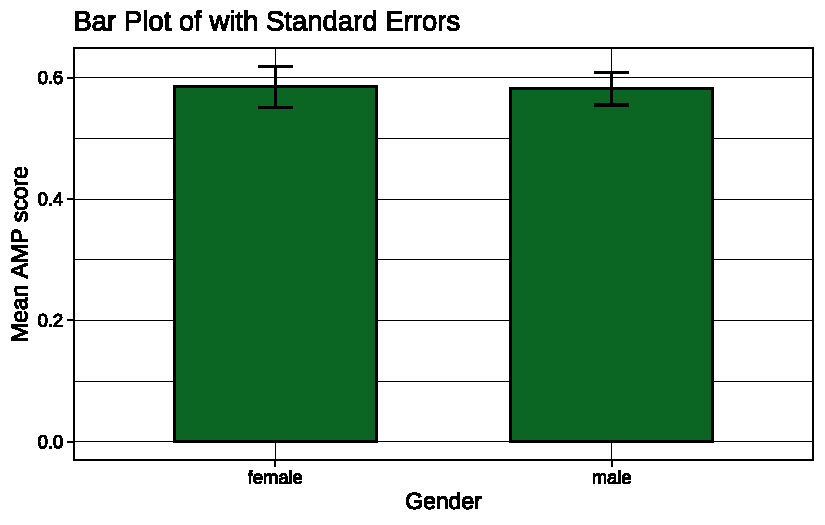
\includegraphics[keepaspectratio]{chapters/visualization_files/figure-pdf/unnamed-chunk-15-1.pdf}}

\section{Exercise: Plot for
self-reports}\label{exercise-plot-for-self-reports}

Make a similar plot for the self-reports.

\begin{itemize}
\tightlist
\item
  Use \texttt{coord\_flip()} to swap the X and Y axes.
\end{itemize}

\begin{itemize}
\tightlist
\item
  Exercise: How to capitalize `Male' and `Female' by wrangling the data
  before plotting?
\end{itemize}

\bookmarksetup{startatroot}

\chapter{Combining plots}\label{combining-plots}

\begin{Shaded}
\begin{Highlighting}[]
\NormalTok{plot\_all }\OtherTok{\textless{}{-}}\NormalTok{ data\_after\_exclusions }\SpecialCharTok{|\textgreater{}}
  \FunctionTok{ggplot}\NormalTok{(}\FunctionTok{aes}\NormalTok{(}\AttributeTok{x =}\NormalTok{ mean\_self\_report,}
             \AttributeTok{y =}\NormalTok{ amp\_score)) }\SpecialCharTok{+}
  \FunctionTok{geom\_point}\NormalTok{() }\SpecialCharTok{+}
  \FunctionTok{geom\_smooth}\NormalTok{(}\AttributeTok{method =} \StringTok{"lm"}\NormalTok{) }\SpecialCharTok{+}
  \FunctionTok{ggtitle}\NormalTok{(}\StringTok{"All"}\NormalTok{)}

\NormalTok{plot\_women }\OtherTok{\textless{}{-}}\NormalTok{ data\_after\_exclusions }\SpecialCharTok{|\textgreater{}}
  \FunctionTok{filter}\NormalTok{(gender }\SpecialCharTok{==} \StringTok{"female"}\NormalTok{) }\SpecialCharTok{|\textgreater{}}
  \FunctionTok{ggplot}\NormalTok{(}\FunctionTok{aes}\NormalTok{(}\AttributeTok{x =}\NormalTok{ mean\_self\_report,}
             \AttributeTok{y =}\NormalTok{ amp\_score)) }\SpecialCharTok{+}
  \FunctionTok{geom\_point}\NormalTok{() }\SpecialCharTok{+}
  \FunctionTok{geom\_smooth}\NormalTok{(}\AttributeTok{method =} \StringTok{"lm"}\NormalTok{) }\SpecialCharTok{+}
  \FunctionTok{ggtitle}\NormalTok{(}\StringTok{"Women"}\NormalTok{)}

\NormalTok{plot\_men }\OtherTok{\textless{}{-}}\NormalTok{ data\_after\_exclusions }\SpecialCharTok{|\textgreater{}}
  \FunctionTok{filter}\NormalTok{(gender }\SpecialCharTok{==} \StringTok{"male"}\NormalTok{) }\SpecialCharTok{|\textgreater{}}
  \FunctionTok{ggplot}\NormalTok{(}\FunctionTok{aes}\NormalTok{(}\AttributeTok{x =}\NormalTok{ mean\_self\_report,}
             \AttributeTok{y =}\NormalTok{ amp\_score)) }\SpecialCharTok{+}
  \FunctionTok{geom\_point}\NormalTok{() }\SpecialCharTok{+}
  \FunctionTok{geom\_smooth}\NormalTok{(}\AttributeTok{method =} \StringTok{"lm"}\NormalTok{) }\SpecialCharTok{+}
  \FunctionTok{ggtitle}\NormalTok{(}\StringTok{"Men"}\NormalTok{)}

\CommentTok{\# combine these plots with different arrangements}
\NormalTok{plot\_women }\SpecialCharTok{+}\NormalTok{ plot\_men}
\end{Highlighting}
\end{Shaded}

\pandocbounded{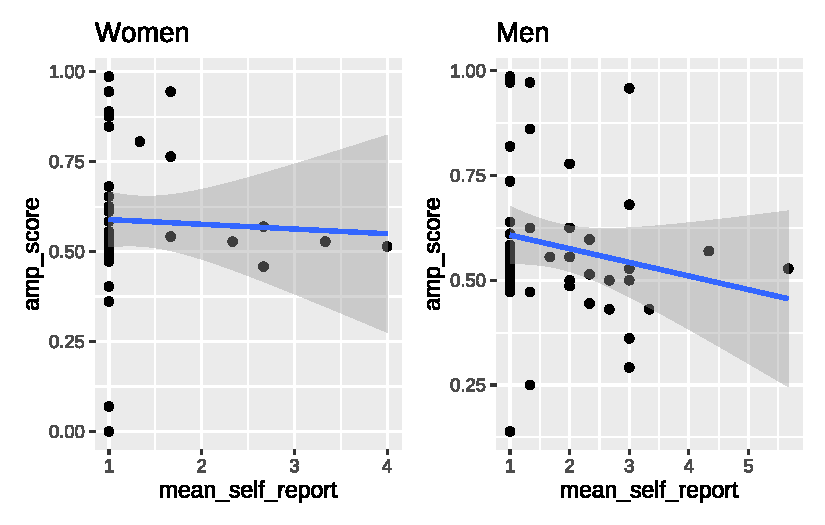
\includegraphics[keepaspectratio]{chapters/visualization_files/figure-pdf/unnamed-chunk-17-1.pdf}}

\begin{Shaded}
\begin{Highlighting}[]
\NormalTok{plot\_women }\SpecialCharTok{+}\NormalTok{ plot\_men }\SpecialCharTok{+} \FunctionTok{plot\_layout}\NormalTok{(}\AttributeTok{ncol =} \DecValTok{1}\NormalTok{)}
\end{Highlighting}
\end{Shaded}

\pandocbounded{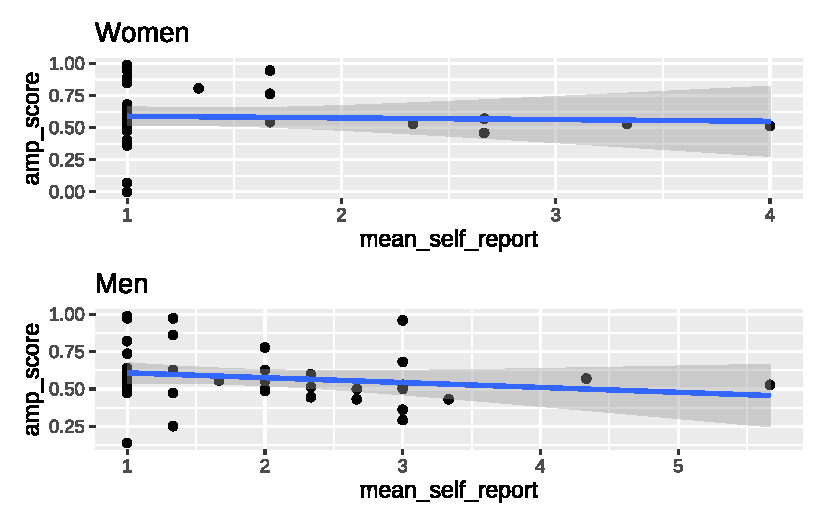
\includegraphics[keepaspectratio]{chapters/visualization_files/figure-pdf/unnamed-chunk-17-2.pdf}}

\begin{Shaded}
\begin{Highlighting}[]
\NormalTok{plot\_all }\SpecialCharTok{/}\NormalTok{ (plot\_women }\SpecialCharTok{+}\NormalTok{ plot\_men)}
\end{Highlighting}
\end{Shaded}

\pandocbounded{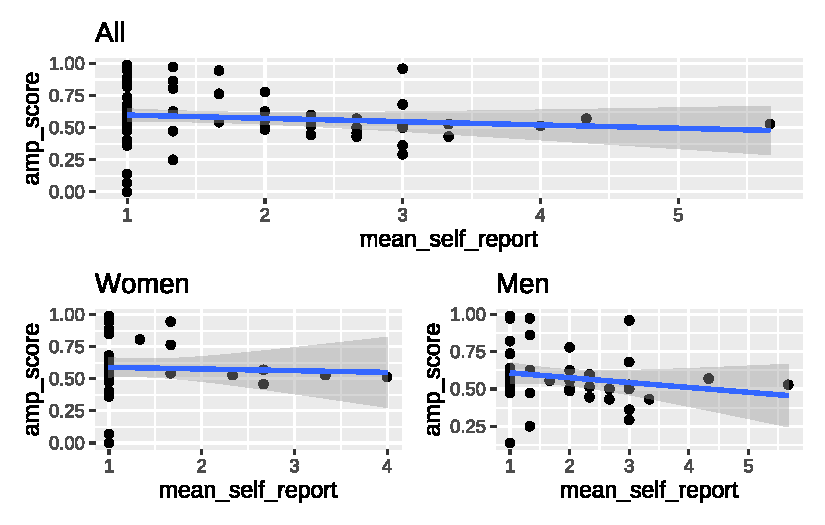
\includegraphics[keepaspectratio]{chapters/visualization_files/figure-pdf/unnamed-chunk-17-3.pdf}}

\bookmarksetup{startatroot}

\chapter{Faceting plots}\label{faceting-plots}

Without repeating yourself, you can also make a plot for different
subsets using \texttt{facet\_wrap()} or \texttt{facet\_grid()}

\begin{Shaded}
\begin{Highlighting}[]
\FunctionTok{ggplot}\NormalTok{(}\AttributeTok{data =}\NormalTok{ data\_after\_exclusions,}
       \FunctionTok{aes}\NormalTok{(}\AttributeTok{x =}\NormalTok{ mean\_self\_report,}
           \AttributeTok{y =}\NormalTok{ amp\_score)) }\SpecialCharTok{+}
  \FunctionTok{geom\_point}\NormalTok{() }\SpecialCharTok{+}
  \FunctionTok{geom\_smooth}\NormalTok{(}\AttributeTok{method =} \StringTok{"lm"}\NormalTok{) }\SpecialCharTok{+}
  \FunctionTok{facet\_wrap}\NormalTok{(}\SpecialCharTok{\textasciitilde{}}\NormalTok{ gender)}
\end{Highlighting}
\end{Shaded}

\pandocbounded{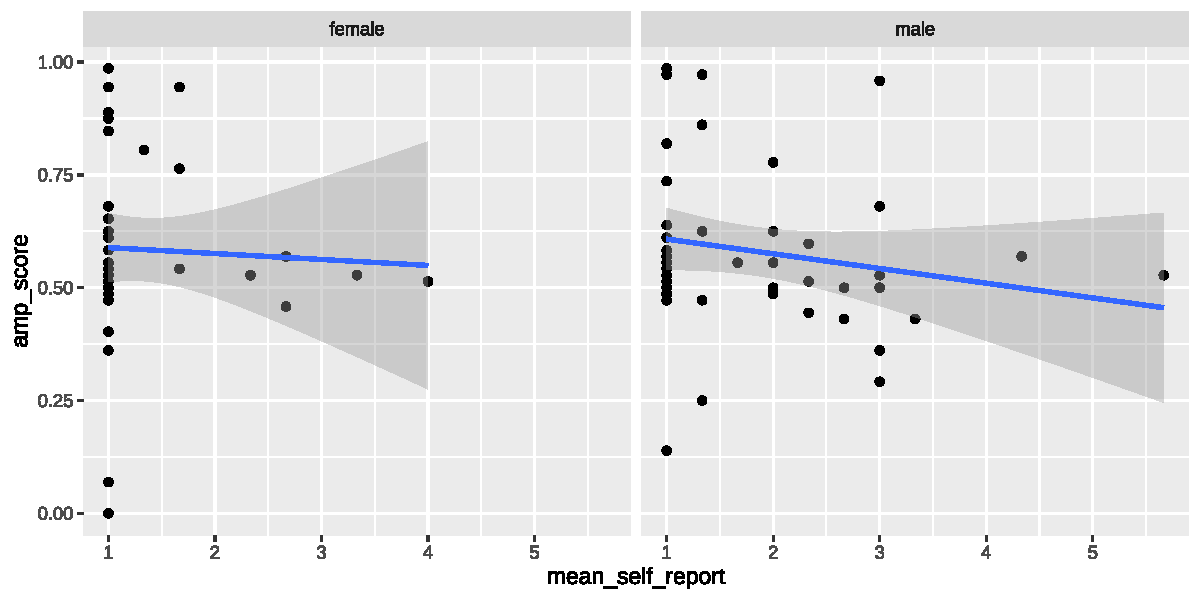
\includegraphics[keepaspectratio]{chapters/visualization_files/figure-pdf/unnamed-chunk-18-1.pdf}}

\section{Exercise}\label{exercise}

Create a plot that assesses the association between self report scores
and AMP scores. By wrangling \texttt{data\_processed} more prior to
plotting, and using \texttt{facet\_grid()}, compare a) men vs women and
b) participants who are 30+ years old vs younger than 30.

Improve the appearance of the plot, including its text, colors, theme,
etc.

\bookmarksetup{startatroot}

\chapter{Session info}\label{session-info}

\begin{Shaded}
\begin{Highlighting}[]
\FunctionTok{sessionInfo}\NormalTok{()}
\end{Highlighting}
\end{Shaded}

\begin{verbatim}
R version 4.5.0 (2025-04-11)
Platform: aarch64-apple-darwin20
Running under: macOS Sequoia 15.5

Matrix products: default
BLAS:   /Library/Frameworks/R.framework/Versions/4.5-arm64/Resources/lib/libRblas.0.dylib 
LAPACK: /Library/Frameworks/R.framework/Versions/4.5-arm64/Resources/lib/libRlapack.dylib;  LAPACK version 3.12.1

locale:
[1] en_US.UTF-8/en_US.UTF-8/en_US.UTF-8/C/en_US.UTF-8/en_US.UTF-8

time zone: Europe/Zurich
tzcode source: internal

attached base packages:
[1] stats     graphics  grDevices utils     datasets  methods   base     

other attached packages:
 [1] kableExtra_1.4.0 knitr_1.50       janitor_2.2.1    patchwork_1.3.0 
 [5] ThemePark_0.0.1  plotrix_3.8-4    tidyr_1.3.1      dplyr_1.1.4     
 [9] scales_1.4.0     datasauRus_0.1.9 ggplot2_3.5.2    readr_2.1.5     

loaded via a namespace (and not attached):
 [1] generics_0.1.4     xml2_1.3.8         lattice_0.22-6     stringi_1.8.7     
 [5] hms_1.1.3          digest_0.6.37      magrittr_2.0.3     evaluate_1.0.3    
 [9] grid_4.5.0         timechange_0.3.0   RColorBrewer_1.1-3 sysfonts_0.8.9    
[13] showtextdb_3.0     fastmap_1.2.0      Matrix_1.7-3       jsonlite_2.0.0    
[17] mgcv_1.9-1         purrr_1.1.0        viridisLite_0.4.2  textshaping_1.0.1 
[21] cli_3.6.5          crayon_1.5.3       rlang_1.1.6        splines_4.5.0     
[25] bit64_4.6.0-1      withr_3.0.2        yaml_2.3.10        parallel_4.5.0    
[29] tools_4.5.0        tzdb_0.5.0         showtext_0.9-7     curl_6.4.0        
[33] vctrs_0.6.5        R6_2.6.1           lifecycle_1.0.4    lubridate_1.9.4   
[37] snakecase_0.11.1   stringr_1.5.1      bit_4.6.0          vroom_1.6.5       
[41] ragg_1.4.0         pkgconfig_2.0.3    pillar_1.11.0      gtable_0.3.6      
[45] glue_1.8.0         systemfonts_1.2.3  xfun_0.52          tibble_3.3.0      
[49] tidyselect_1.2.1   rstudioapi_0.17.1  farver_2.1.2       nlme_3.1-168      
[53] htmltools_0.5.8.1  rmarkdown_2.29     svglite_2.2.1      labeling_0.4.3    
[57] compiler_4.5.0    
\end{verbatim}

\bookmarksetup{startatroot}

\chapter{License and citation}\label{license-and-citation}

© Ian Hussey (2025)

Text and figures are licensed under a
\href{https://creativecommons.org/licenses/by/4.0/}{Creative Commons
Attribution 4.0 (CC BY 4.0)} license.

Code is licensed under the
\href{https://opensource.org/licenses/MIT}{MIT License}.

You are free to copy, share, adapt, and reuse the contents of this book
--- text, figures, and code --- for any purpose, including commercial
use, provided you cite it.

Citation:

Hussey, I. (2025) Improving your statistical inferences using Monte
Carlo simulation studies in tidyverse.
github.com/ianhussey/improving-your-statistical-inferences-through-monte-carlo-simulation-studies




\end{document}
